\documentclass[UTF8]{ctexart}

\title{\Large 中国科学技术大学\\{\Large 电子技术实验III}\\{\Large 实验报告}}
\usepackage{amsmath}
\usepackage{amsfonts}
\usepackage{amssymb}
\usepackage{bm}
\usepackage{enumerate}
\usepackage{geometry}
\geometry{left=2.5cm,right=2.5cm,top=3.5cm,bottom=3.5cm}
\usepackage{fancyhdr}
\usepackage{lastpage}
\pagestyle{fancy}
\fancyhead[l]{ }
\fancyhead[r]{ }
\fancyhead[C]{
	\begin{tabular}{cclclc}
         & \multicolumn{4}{c}{\textbf{小信号调谐放大器\quad 实验报告}}                                    &            \vspace{1ex}\\
信息科学技术学院 & \multicolumn{2}{c}{PB22051030 王旭东} & \multicolumn{2}{c}{PB22051031 李毅} & 2024年11月1日
\end{tabular}
}
\fancyfoot[C]{ 第 {\thepage} 页,共 \pageref{LastPage} 页}
\setlength{\headheight}{29.83218pt}
\setlength{\abovecaptionskip}{1em}
\renewcommand{\headrulewidth}{1pt}
\usepackage{graphicx,tikz}
\usepackage{geometry}
\usepackage[hidelinks]{hyperref}
\usepackage{multicol}
\usepackage{multirow}
\usepackage{ragged2e}
\usepackage[square,comma,numbers,super]{natbib}
\bibliographystyle{unsrt}
\usepackage{siunitx}
\usepackage{subcaption}
\usepackage{wrapfig}
\usepackage{xcolor}
\usepackage{cite}
\usepackage{booktabs}
\usepackage{diagbox}
\usepackage{listings}
\usepackage{makecell}
\usepackage[final]{pdfpages}
\usepackage[T1]{fontenc}
\usepackage{float}
\makeatletter
\newcommand\dlmu[2][4cm]{\hskip1pt\underline{\hb@xt@ #1{\hss#2\hss}}\hskip3pt}
\makeatother
\ctexset{
    % 修改 section。
    section={   
        name={,\quad},
        number={\empty},
        format=\bfseries\centering\zihao{3}, % 设置 section 标题为黑体、右对齐、小4号字
        aftername=\hspace{0pt},
        beforeskip=2ex,
        afterskip=2ex
    },
    % 修改 subsection。
    subsection={   
        name={,\quad},
        number={\arabic{section}.\arabic{subsection}},
        format=\bfseries\zihao{4}, % 设置 subsection 标题为黑体、5号字
        aftername=\hspace{0pt},
        beforeskip=1ex,
        afterskip=2ex
    },
    % 修改 subsubsection。
    subsubsection={   
        name={,\quad},
        number={\arabic{section}.\arabic{subsection}.\arabic{subsubsection}},
        format=\bfseries\zihao{5}, % 设置 subsection 标题为黑体、5号字
        aftername=\hspace{0pt},
        beforeskip=1ex,
        afterskip=1ex
    }
}
\newcommand{\subsubsubsection}[1]{\paragraph{#1}\mbox{}\\}
\setcounter{secnumdepth}{4} % how many sectioning levels to assign numbers to
\setcounter{tocdepth}{4} % how many sectioning levels to show in ToC
% Style definition file generated by highlight 4.8, http://www.andre-simon.de/ 
% highlight theme: Bright
\newcommand{\hldef}[1]{\textcolor[rgb]{0.2,0,0.4}{#1}}
\newcommand{\hlnum}[1]{\textcolor[rgb]{0.2,0.73,0.02}{#1}}
\newcommand{\hlesc}[1]{\textcolor[rgb]{0.65,0.09,0.38}{#1}}
\newcommand{\hlsng}[1]{\textcolor[rgb]{0.09,0.38,0.65}{#1}}
\newcommand{\hlpps}[1]{\textcolor[rgb]{0.4,0.2,0}{#1}}
\newcommand{\hlslc}[1]{\textcolor[rgb]{0,0.4,0.2}{#1}}
\newcommand{\hlcom}[1]{\textcolor[rgb]{0,0.4,0.2}{#1}}
\newcommand{\hlppc}[1]{\textcolor[rgb]{0.33,0.45,0.69}{#1}}
\newcommand{\hlopt}[1]{\textcolor[rgb]{0.33,0.33,0.33}{#1}}
\newcommand{\hlipl}[1]{\textcolor[rgb]{0.65,0.09,0.38}{#1}}
\newcommand{\hllin}[1]{\textcolor[rgb]{0.6,0.6,0.6}{#1}}
\newcommand{\hlerr}[1]{\textcolor[rgb]{1,0,0}{\bf{#1}}}
\newcommand{\hlerm}[1]{\marginpar{\small\itshape\color{red}#1}}
\newcommand{\hlkwa}[1]{\textcolor[rgb]{1,0.19,0.19}{#1}}
\newcommand{\hlkwb}[1]{\textcolor[rgb]{0.96,0.55,0.14}{#1}}
\newcommand{\hlkwc}[1]{\textcolor[rgb]{0,0,1}{#1}}
\newcommand{\hlkwd}[1]{\textcolor[rgb]{0.82,0.11,0.93}{#1}}
\newcommand{\hlkwe}[1]{\textcolor[rgb]{0.87,0.51,0.05}{#1}}
\newcommand{\hlkwf}[1]{\textcolor[rgb]{0.47,0.42,0.72}{#1}}
\definecolor{bgcolor}{rgb}{1,1,1}


\begin{document}

\begin{titlepage}
    \begin{center}

        \zihao{1}\textbf{电子技术实验III\quad 实验报告}\\
        \vspace{0.5cm}
        \zihao{2}\textbf{实验一\quad 小信号调谐放大器}
    
        \vspace{1.5cm}
        \resizebox{4cm}{4cm}{
\begin{tikzpicture}[y=0.80pt,x=0.80pt,yscale=-1, xscale=1,even odd rule]
    \definecolor{ustcblue}{RGB}{0,92,170}
    \path[fill=ustcblue] (2074.0000,1058.0000) .. controls (2074.0000,497.0000) and (1619.0000,42.0000) .. (1058.0000,42.0000) .. controls (497.0000,42.0000) and (42.0000,497.0000) .. (42.0000,1058.0000) .. controls (42.0000,1619.0000) and (497.0000,2074.0000) .. (1058.0000,2074.0000) .. controls (1619.0000,2074.0000) and (2074.0000,1619.0000) .. (2074.0000,1058.0000) -- cycle(2040.0000,1058.0000) .. controls (2040.0000,516.0000) and (1601.0000,76.0000) .. (1058.0000,76.0000) .. controls (516.0000,76.0000) and (76.0000,516.0000) .. (76.0000,1058.0000) .. controls (76.0000,1601.0000) and (516.0000,2040.0000) .. (1058.0000,2040.0000) .. controls (1601.0000,2040.0000) and (2040.0000,1601.0000) .. (2040.0000,1058.0000) -- cycle;
    \path[fill=ustcblue] (1187.0000,605.0000) .. controls (1116.0000,587.0000) and (1041.0000,574.0000) .. (960.0000,570.0000) .. controls (996.0000,578.0000) and (1075.0000,649.0000) .. (1089.0000,670.0000) .. controls (1097.0000,682.0000) and (1072.0000,636.0000) .. (1083.0000,621.0000) .. controls (1094.0000,606.0000) and (1154.0000,601.0000) .. (1187.0000,605.0000) -- cycle;
    \path[fill=ustcblue] (1054.0000,1385.0000) -- (1065.0000,1385.0000) -- (1092.0000,1385.0000) .. controls (1072.0000,1290.0000) and (1254.0000,1329.0000) .. (1321.0000,1337.0000) .. controls (1412.0000,1348.0000) and (1455.0000,1343.0000) .. (1479.0000,1344.0000) .. controls (1479.0000,1344.0000) and (1479.0000,1346.0000) .. (1466.0000,1337.0000) .. controls (1452.0000,1327.0000) and (1437.0000,1307.0000) .. (1437.0000,1307.0000) .. controls (1350.0000,1306.0000) and (1304.0000,1298.0000) .. (1228.0000,1269.0000) .. controls (1187.0000,1254.0000) and (1081.0000,1234.0000) .. (1061.0000,1327.0000) -- (1058.0000,1327.0000) .. controls (1038.0000,1234.0000) and (932.0000,1254.0000) .. (891.0000,1269.0000) .. controls (815.0000,1298.0000) and (769.0000,1306.0000) .. (682.0000,1307.0000) .. controls (682.0000,1307.0000) and (667.0000,1327.0000) .. (654.0000,1337.0000) .. controls (640.0000,1346.0000) and (640.0000,1344.0000) .. (640.0000,1344.0000) .. controls (664.0000,1343.0000) and (707.0000,1348.0000) .. (798.0000,1337.0000) .. controls (865.0000,1329.0000) and (1047.0000,1290.0000) .. (1027.0000,1385.0000) -- (1054.0000,1385.0000) -- cycle;
    \path[fill=ustcblue] (1385.0000,1274.0000) .. controls (1438.0000,1164.0000) and (1477.0000,1012.0000) .. (1410.0000,870.0000) .. controls (1349.0000,741.0000) and (1208.0000,672.0000) .. (1132.0000,647.0000) .. controls (1142.0000,652.0000) and (1149.0000,656.0000) .. (1166.0000,666.0000) .. controls (1200.0000,691.0000) and (1226.0000,726.0000) .. (1237.0000,767.0000) .. controls (1238.0000,771.0000) and (1239.0000,775.0000) .. (1239.0000,779.0000) .. controls (1242.0000,792.0000) and (1243.0000,805.0000) .. (1243.0000,818.0000) .. controls (1243.0000,821.0000) and (1243.0000,823.0000) .. (1243.0000,825.0000) .. controls (1244.0000,890.0000) and (1226.0000,962.0000) .. (1184.0000,1024.0000) .. controls (1088.0000,1170.0000) and (897.0000,1248.0000) .. (851.0000,1272.0000) .. controls (972.0000,1238.0000) and (1141.0000,1125.0000) .. (1195.0000,1035.0000) .. controls (1253.0000,948.0000) and (1265.0000,837.0000) .. (1249.0000,762.0000) .. controls (1313.0000,880.0000) and (1312.0000,1057.0000) .. (1098.0000,1255.0000) .. controls (1158.0000,1219.0000) and (1257.0000,1106.0000) .. (1284.0000,1007.0000) .. controls (1321.0000,880.0000) and (1279.0000,773.0000) .. (1230.0000,715.0000) .. controls (1282.0000,770.0000) and (1350.0000,875.0000) .. (1348.0000,977.0000) .. controls (1349.0000,1032.0000) and (1312.0000,1170.0000) .. (1251.0000,1263.0000) .. controls (1304.0000,1188.0000) and (1363.0000,1085.0000) .. (1363.0000,968.0000) .. controls (1363.0000,859.0000) and (1290.0000,752.0000) .. (1231.0000,702.0000) .. controls (1292.0000,741.0000) and (1365.0000,803.0000) .. (1405.0000,894.0000) .. controls (1467.0000,1037.0000) and (1411.0000,1193.0000) .. (1385.0000,1274.0000) -- cycle;
    \path[fill=ustcblue] (719.0000,910.0000) -- (719.0000,1019.0000) -- (692.0000,1019.0000) -- (692.0000,948.0000) .. controls (688.0000,951.0000) and (684.0000,954.0000) .. (679.0000,957.0000) .. controls (675.0000,959.0000) and (670.0000,961.0000) .. (664.0000,963.0000) -- (664.0000,939.0000) .. controls (673.0000,936.0000) and (680.0000,932.0000) .. (685.0000,927.0000) .. controls (690.0000,923.0000) and (694.0000,917.0000) .. (697.0000,910.0000) -- (719.0000,910.0000) -- cycle;
    \path[fill=ustcblue] (758.0000,995.0000) -- (784.0000,991.0000) .. controls (785.0000,995.0000) and (786.0000,998.0000) .. (787.0000,1000.0000) .. controls (789.0000,1002.0000) and (791.0000,1002.0000) .. (793.0000,1002.0000) .. controls (798.0000,1002.0000) and (801.0000,1000.0000) .. (803.0000,995.0000) .. controls (805.0000,992.0000) and (807.0000,984.0000) .. (807.0000,973.0000) .. controls (804.0000,976.0000) and (801.0000,979.0000) .. (798.0000,981.0000) .. controls (794.0000,982.0000) and (790.0000,983.0000) .. (786.0000,983.0000) .. controls (777.0000,983.0000) and (770.0000,980.0000) .. (764.0000,973.0000) .. controls (759.0000,966.0000) and (756.0000,958.0000) .. (756.0000,947.0000) .. controls (756.0000,940.0000) and (757.0000,934.0000) .. (760.0000,928.0000) .. controls (763.0000,922.0000) and (767.0000,918.0000) .. (772.0000,915.0000) .. controls (778.0000,912.0000) and (784.0000,910.0000) .. (792.0000,910.0000) .. controls (802.0000,910.0000) and (809.0000,912.0000) .. (815.0000,916.0000) .. controls (821.0000,920.0000) and (826.0000,925.0000) .. (829.0000,933.0000) .. controls (832.0000,941.0000) and (834.0000,952.0000) .. (834.0000,965.0000) .. controls (834.0000,984.0000) and (830.0000,998.0000) .. (823.0000,1007.0000) .. controls (816.0000,1016.0000) and (806.0000,1020.0000) .. (793.0000,1020.0000) .. controls (786.0000,1020.0000) and (780.0000,1019.0000) .. (775.0000,1018.0000) .. controls (771.0000,1016.0000) and (767.0000,1013.0000) .. (764.0000,1009.0000) .. controls (761.0000,1005.0000) and (759.0000,1001.0000) .. (758.0000,995.0000) -- cycle(806.0000,947.0000) .. controls (806.0000,942.0000) and (805.0000,937.0000) .. (803.0000,934.0000) .. controls (800.0000,931.0000) and (797.0000,929.0000) .. (793.0000,929.0000) .. controls (790.0000,929.0000) and (787.0000,930.0000) .. (784.0000,933.0000) .. controls (782.0000,936.0000) and (781.0000,941.0000) .. (781.0000,947.0000) .. controls (781.0000,953.0000) and (782.0000,957.0000) .. (784.0000,960.0000) .. controls (787.0000,963.0000) and (790.0000,965.0000) .. (793.0000,965.0000) .. controls (797.0000,965.0000) and (800.0000,964.0000) .. (803.0000,960.0000) .. controls (805.0000,957.0000) and (806.0000,953.0000) .. (806.0000,947.0000) -- cycle;
    \path[fill=ustcblue] (865.0000,912.0000) -- (928.0000,912.0000) -- (928.0000,936.0000) -- (885.0000,936.0000) -- (883.0000,952.0000) .. controls (886.0000,950.0000) and (889.0000,949.0000) .. (892.0000,948.0000) .. controls (894.0000,948.0000) and (897.0000,947.0000) .. (900.0000,947.0000) .. controls (910.0000,947.0000) and (917.0000,950.0000) .. (923.0000,957.0000) .. controls (929.0000,963.0000) and (932.0000,971.0000) .. (932.0000,981.0000) .. controls (932.0000,988.0000) and (931.0000,995.0000) .. (928.0000,1001.0000) .. controls (925.0000,1007.0000) and (920.0000,1012.0000) .. (915.0000,1015.0000) .. controls (909.0000,1019.0000) and (902.0000,1020.0000) .. (893.0000,1020.0000) .. controls (887.0000,1020.0000) and (881.0000,1020.0000) .. (877.0000,1018.0000) .. controls (872.0000,1017.0000) and (869.0000,1015.0000) .. (866.0000,1012.0000) .. controls (862.0000,1010.0000) and (860.0000,1007.0000) .. (858.0000,1003.0000) .. controls (856.0000,1000.0000) and (854.0000,996.0000) .. (853.0000,991.0000) -- (880.0000,988.0000) .. controls (880.0000,993.0000) and (882.0000,996.0000) .. (884.0000,999.0000) .. controls (887.0000,1001.0000) and (889.0000,1003.0000) .. (893.0000,1003.0000) .. controls (897.0000,1003.0000) and (900.0000,1001.0000) .. (902.0000,998.0000) .. controls (904.0000,995.0000) and (906.0000,990.0000) .. (906.0000,984.0000) .. controls (906.0000,977.0000) and (904.0000,973.0000) .. (902.0000,970.0000) .. controls (900.0000,967.0000) and (896.0000,965.0000) .. (892.0000,965.0000) .. controls (890.0000,965.0000) and (887.0000,966.0000) .. (885.0000,968.0000) .. controls (883.0000,969.0000) and (881.0000,970.0000) .. (879.0000,973.0000) -- (856.0000,969.0000) -- (865.0000,912.0000) -- cycle;
    \path[fill=ustcblue] (968.0000,961.0000) .. controls (964.0000,959.0000) and (960.0000,956.0000) .. (959.0000,953.0000) .. controls (956.0000,949.0000) and (955.0000,944.0000) .. (955.0000,939.0000) .. controls (955.0000,930.0000) and (958.0000,923.0000) .. (966.0000,917.0000) .. controls (972.0000,913.0000) and (980.0000,910.0000) .. (989.0000,910.0000) .. controls (1002.0000,910.0000) and (1011.0000,913.0000) .. (1017.0000,919.0000) .. controls (1024.0000,924.0000) and (1027.0000,931.0000) .. (1027.0000,939.0000) .. controls (1027.0000,944.0000) and (1025.0000,948.0000) .. (1023.0000,952.0000) .. controls (1021.0000,956.0000) and (1018.0000,958.0000) .. (1014.0000,961.0000) .. controls (1019.0000,964.0000) and (1023.0000,968.0000) .. (1026.0000,972.0000) .. controls (1028.0000,977.0000) and (1030.0000,982.0000) .. (1030.0000,988.0000) .. controls (1030.0000,993.0000) and (1029.0000,998.0000) .. (1026.0000,1002.0000) .. controls (1024.0000,1007.0000) and (1021.0000,1011.0000) .. (1018.0000,1013.0000) .. controls (1015.0000,1016.0000) and (1011.0000,1018.0000) .. (1006.0000,1019.0000) .. controls (1002.0000,1020.0000) and (997.0000,1020.0000) .. (991.0000,1020.0000) .. controls (981.0000,1020.0000) and (973.0000,1019.0000) .. (968.0000,1017.0000) .. controls (963.0000,1014.0000) and (959.0000,1010.0000) .. (956.0000,1005.0000) .. controls (953.0000,1000.0000) and (952.0000,994.0000) .. (952.0000,987.0000) .. controls (952.0000,981.0000) and (953.0000,976.0000) .. (956.0000,972.0000) .. controls (958.0000,967.0000) and (962.0000,964.0000) .. (968.0000,961.0000) -- cycle(980.0000,941.0000) .. controls (980.0000,944.0000) and (981.0000,947.0000) .. (983.0000,949.0000) .. controls (985.0000,952.0000) and (987.0000,953.0000) .. (991.0000,953.0000) .. controls (994.0000,953.0000) and (996.0000,952.0000) .. (998.0000,950.0000) .. controls (1000.0000,947.0000) and (1001.0000,944.0000) .. (1001.0000,941.0000) .. controls (1001.0000,937.0000) and (1000.0000,934.0000) .. (998.0000,932.0000) .. controls (996.0000,930.0000) and (994.0000,928.0000) .. (990.0000,928.0000) .. controls (987.0000,928.0000) and (985.0000,930.0000) .. (983.0000,932.0000) .. controls (981.0000,934.0000) and (980.0000,937.0000) .. (980.0000,941.0000) -- cycle(978.0000,986.0000) .. controls (978.0000,991.0000) and (979.0000,995.0000) .. (982.0000,998.0000) .. controls (984.0000,1001.0000) and (987.0000,1002.0000) .. (991.0000,1002.0000) .. controls (994.0000,1002.0000) and (997.0000,1001.0000) .. (999.0000,998.0000) .. controls (1002.0000,995.0000) and (1003.0000,991.0000) .. (1003.0000,986.0000) .. controls (1003.0000,982.0000) and (1002.0000,978.0000) .. (999.0000,975.0000) .. controls (997.0000,972.0000) and (994.0000,970.0000) .. (990.0000,970.0000) .. controls (987.0000,970.0000) and (984.0000,972.0000) .. (982.0000,975.0000) .. controls (979.0000,977.0000) and (978.0000,981.0000) .. (978.0000,986.0000) -- cycle;
    \path[fill=ustcblue] (1058.0000,519.0000) .. controls (1356.0000,519.0000) and (1597.0000,761.0000) .. (1597.0000,1058.0000) .. controls (1597.0000,1356.0000) and (1356.0000,1597.0000) .. (1058.0000,1597.0000) .. controls (761.0000,1597.0000) and (519.0000,1356.0000) .. (519.0000,1058.0000) .. controls (519.0000,761.0000) and (761.0000,519.0000) .. (1058.0000,519.0000) -- cycle(1058.0000,541.0000) .. controls (1344.0000,541.0000) and (1576.0000,773.0000) .. (1576.0000,1058.0000) .. controls (1576.0000,1344.0000) and (1344.0000,1576.0000) .. (1058.0000,1576.0000) .. controls (773.0000,1576.0000) and (541.0000,1344.0000) .. (541.0000,1058.0000) .. controls (541.0000,773.0000) and (773.0000,541.0000) .. (1058.0000,541.0000) -- cycle;
    \path[fill=ustcblue] (197.0000,705.0000) .. controls (212.0000,690.0000) and (225.0000,682.0000) .. (235.0000,683.0000) -- (255.0000,694.0000) -- (265.0000,657.0000) .. controls (271.0000,646.0000) and (277.0000,640.0000) .. (281.0000,641.0000) -- (287.0000,645.0000) .. controls (292.0000,656.0000) and (295.0000,667.0000) .. (298.0000,678.0000) -- (300.0000,697.0000) .. controls (304.0000,687.0000) and (310.0000,680.0000) .. (319.0000,675.0000) -- (324.0000,675.0000) .. controls (330.0000,678.0000) and (330.0000,686.0000) .. (326.0000,701.0000) .. controls (325.0000,706.0000) and (327.0000,719.0000) .. (332.0000,741.0000) .. controls (350.0000,751.0000) and (361.0000,760.0000) .. (365.0000,768.0000) .. controls (375.0000,775.0000) and (380.0000,779.0000) .. (381.0000,781.0000) .. controls (379.0000,785.0000) and (371.0000,785.0000) .. (356.0000,781.0000) .. controls (352.0000,781.0000) and (342.0000,780.0000) .. (328.0000,777.0000) .. controls (326.0000,785.0000) and (320.0000,789.0000) .. (311.0000,787.0000) .. controls (305.0000,799.0000) and (292.0000,805.0000) .. (272.0000,807.0000) -- (248.0000,802.0000) .. controls (237.0000,797.0000) and (233.0000,793.0000) .. (235.0000,787.0000) .. controls (240.0000,781.0000) and (245.0000,778.0000) .. (249.0000,777.0000) .. controls (246.0000,768.0000) and (245.0000,754.0000) .. (246.0000,736.0000) -- (244.0000,734.0000) .. controls (210.0000,720.0000) and (194.0000,711.0000) .. (197.0000,705.0000) -- cycle(283.0000,712.0000) -- (286.0000,713.0000) .. controls (290.0000,716.0000) and (292.0000,717.0000) .. (293.0000,716.0000) .. controls (290.0000,696.0000) and (286.0000,681.0000) .. (280.0000,671.0000) -- (279.0000,670.0000) .. controls (274.0000,684.0000) and (272.0000,696.0000) .. (273.0000,705.0000) -- (283.0000,712.0000) -- cycle(277.0000,772.0000) .. controls (293.0000,776.0000) and (302.0000,777.0000) .. (303.0000,774.0000) -- (304.0000,773.0000) -- (299.0000,761.0000) -- (299.0000,761.0000) -- (293.0000,758.0000) -- (288.0000,756.0000) -- (284.0000,753.0000) -- (278.0000,751.0000) -- (271.0000,747.0000) -- (271.0000,747.0000) .. controls (269.0000,752.0000) and (271.0000,761.0000) .. (277.0000,772.0000) -- cycle(379.0000,408.0000) .. controls (391.0000,398.0000) and (401.0000,393.0000) .. (411.0000,393.0000) .. controls (426.0000,398.0000) and (441.0000,408.0000) .. (458.0000,423.0000) -- (471.0000,436.0000) -- (501.0000,461.0000) -- (522.0000,479.0000) .. controls (530.0000,486.0000) and (534.0000,495.0000) .. (533.0000,504.0000) .. controls (531.0000,516.0000) and (527.0000,526.0000) .. (519.0000,535.0000) -- (492.0000,546.0000) -- (486.0000,560.0000) -- (486.0000,560.0000) -- (472.0000,581.0000) .. controls (468.0000,585.0000) and (462.0000,587.0000) .. (454.0000,587.0000) -- (454.0000,588.0000) .. controls (457.0000,592.0000) and (457.0000,596.0000) .. (455.0000,598.0000) .. controls (449.0000,602.0000) and (442.0000,600.0000) .. (432.0000,593.0000) .. controls (421.0000,577.0000) and (410.0000,564.0000) .. (398.0000,555.0000) -- (367.0000,534.0000) .. controls (352.0000,517.0000) and (347.0000,507.0000) .. (350.0000,504.0000) .. controls (347.0000,491.0000) and (347.0000,480.0000) .. (351.0000,471.0000) .. controls (353.0000,451.0000) and (363.0000,430.0000) .. (379.0000,408.0000) -- cycle(384.0000,508.0000) .. controls (382.0000,490.0000) and (385.0000,477.0000) .. (393.0000,467.0000) .. controls (401.0000,461.0000) and (407.0000,460.0000) .. (408.0000,462.0000) .. controls (415.0000,466.0000) and (421.0000,473.0000) .. (425.0000,484.0000) .. controls (428.0000,482.0000) and (431.0000,480.0000) .. (435.0000,478.0000) .. controls (437.0000,478.0000) and (440.0000,478.0000) .. (443.0000,475.0000) -- (445.0000,474.0000) .. controls (457.0000,464.0000) and (465.0000,461.0000) .. (469.0000,464.0000) -- (471.0000,464.0000) -- (473.0000,465.0000) .. controls (477.0000,473.0000) and (478.0000,482.0000) .. (476.0000,490.0000) .. controls (476.0000,512.0000) and (471.0000,531.0000) .. (461.0000,546.0000) -- (459.0000,549.0000) .. controls (454.0000,551.0000) and (450.0000,551.0000) .. (445.0000,548.0000) -- (444.0000,548.0000) .. controls (440.0000,544.0000) and (438.0000,537.0000) .. (436.0000,527.0000) -- (436.0000,527.0000) -- (432.0000,532.0000) -- (431.0000,533.0000) .. controls (426.0000,536.0000) and (420.0000,536.0000) .. (413.0000,533.0000) .. controls (408.0000,529.0000) and (408.0000,518.0000) .. (414.0000,499.0000) -- (407.0000,488.0000) -- (406.0000,487.0000) .. controls (395.0000,507.0000) and (392.0000,519.0000) .. (395.0000,522.0000) .. controls (399.0000,525.0000) and (403.0000,531.0000) .. (409.0000,539.0000) -- (411.0000,543.0000) -- (415.0000,547.0000) -- (434.0000,562.0000) -- (443.0000,573.0000) .. controls (449.0000,578.0000) and (455.0000,577.0000) .. (463.0000,569.0000) .. controls (473.0000,555.0000) and (477.0000,547.0000) .. (476.0000,545.0000) -- (468.0000,545.0000) -- (466.0000,543.0000) -- (468.0000,541.0000) -- (483.0000,534.0000) -- (492.0000,517.0000) -- (493.0000,517.0000) -- (493.0000,517.0000) -- (494.0000,523.0000) -- (502.0000,515.0000) .. controls (508.0000,502.0000) and (509.0000,493.0000) .. (504.0000,487.0000) .. controls (502.0000,485.0000) and (498.0000,480.0000) .. (490.0000,473.0000) -- (482.0000,465.0000) -- (476.0000,460.0000) -- (461.0000,449.0000) -- (443.0000,433.0000) -- (403.0000,410.0000) .. controls (399.0000,409.0000) and (395.0000,411.0000) .. (392.0000,414.0000) -- (385.0000,422.0000) .. controls (373.0000,435.0000) and (368.0000,451.0000) .. (369.0000,468.0000) .. controls (367.0000,485.0000) and (372.0000,498.0000) .. (384.0000,508.0000) -- cycle(433.0000,503.0000) -- (434.0000,505.0000) -- (433.0000,500.0000) -- (429.0000,495.0000) .. controls (430.0000,499.0000) and (431.0000,501.0000) .. (433.0000,503.0000) -- cycle(443.0000,480.0000) -- (451.0000,487.0000) -- (456.0000,494.0000) -- (458.0000,488.0000) .. controls (458.0000,484.0000) and (457.0000,481.0000) .. (455.0000,479.0000) .. controls (451.0000,478.0000) and (448.0000,478.0000) .. (446.0000,478.0000) -- (443.0000,480.0000) -- cycle(418.0000,522.0000) -- (420.0000,524.0000) -- (422.0000,524.0000) -- (422.0000,524.0000) .. controls (423.0000,521.0000) and (423.0000,517.0000) .. (421.0000,513.0000) -- (419.0000,512.0000) -- (418.0000,515.0000) -- (418.0000,522.0000) -- cycle(642.0000,203.0000) .. controls (647.0000,201.0000) and (655.0000,204.0000) .. (666.0000,210.0000) .. controls (672.0000,214.0000) and (677.0000,221.0000) .. (681.0000,228.0000) -- (687.0000,237.0000) .. controls (700.0000,243.0000) and (710.0000,248.0000) .. (716.0000,253.0000) .. controls (730.0000,254.0000) and (737.0000,256.0000) .. (738.0000,258.0000) .. controls (741.0000,262.0000) and (737.0000,269.0000) .. (724.0000,278.0000) .. controls (717.0000,286.0000) and (715.0000,292.0000) .. (717.0000,296.0000) -- (721.0000,309.0000) -- (722.0000,317.0000) .. controls (725.0000,324.0000) and (729.0000,337.0000) .. (732.0000,356.0000) -- (738.0000,376.0000) -- (740.0000,380.0000) -- (740.0000,383.0000) -- (739.0000,384.0000) .. controls (727.0000,380.0000) and (714.0000,366.0000) .. (700.0000,342.0000) -- (694.0000,331.0000) -- (691.0000,328.0000) .. controls (690.0000,333.0000) and (681.0000,342.0000) .. (665.0000,355.0000) .. controls (660.0000,357.0000) and (655.0000,358.0000) .. (652.0000,357.0000) -- (650.0000,355.0000) -- (648.0000,352.0000) -- (647.0000,350.0000) -- (645.0000,345.0000) .. controls (644.0000,342.0000) and (645.0000,337.0000) .. (649.0000,331.0000) .. controls (653.0000,311.0000) and (655.0000,298.0000) .. (654.0000,292.0000) -- (645.0000,285.0000) .. controls (642.0000,295.0000) and (640.0000,308.0000) .. (639.0000,323.0000) .. controls (638.0000,340.0000) and (638.0000,349.0000) .. (639.0000,350.0000) -- (641.0000,355.0000) .. controls (646.0000,365.0000) and (653.0000,374.0000) .. (660.0000,382.0000) .. controls (661.0000,386.0000) and (662.0000,389.0000) .. (661.0000,389.0000) -- (659.0000,390.0000) .. controls (649.0000,390.0000) and (641.0000,384.0000) .. (634.0000,372.0000) -- (633.0000,372.0000) -- (631.0000,375.0000) .. controls (631.0000,377.0000) and (628.0000,384.0000) .. (622.0000,395.0000) .. controls (620.0000,400.0000) and (615.0000,404.0000) .. (607.0000,408.0000) .. controls (602.0000,407.0000) and (597.0000,404.0000) .. (593.0000,399.0000) -- (592.0000,395.0000) .. controls (590.0000,391.0000) and (591.0000,379.0000) .. (596.0000,360.0000) -- (600.0000,334.0000) -- (599.0000,332.0000) .. controls (590.0000,345.0000) and (583.0000,352.0000) .. (580.0000,354.0000) .. controls (576.0000,357.0000) and (572.0000,355.0000) .. (570.0000,351.0000) .. controls (567.0000,346.0000) and (569.0000,338.0000) .. (574.0000,328.0000) -- (581.0000,303.0000) -- (586.0000,278.0000) .. controls (587.0000,272.0000) and (587.0000,264.0000) .. (584.0000,255.0000) -- (588.0000,245.0000) .. controls (593.0000,241.0000) and (598.0000,241.0000) .. (604.0000,247.0000) -- (605.0000,247.0000) .. controls (606.0000,255.0000) and (605.0000,263.0000) .. (603.0000,272.0000) .. controls (598.0000,285.0000) and (594.0000,297.0000) .. (591.0000,309.0000) -- (580.0000,337.0000) -- (581.0000,337.0000) -- (583.0000,336.0000) .. controls (586.0000,332.0000) and (595.0000,323.0000) .. (609.0000,309.0000) .. controls (607.0000,299.0000) and (607.0000,288.0000) .. (611.0000,276.0000) .. controls (611.0000,275.0000) and (612.0000,274.0000) .. (614.0000,273.0000) .. controls (619.0000,270.0000) and (628.0000,272.0000) .. (642.0000,279.0000) .. controls (642.0000,273.0000) and (642.0000,268.0000) .. (639.0000,263.0000) -- (638.0000,263.0000) -- (637.0000,264.0000) -- (636.0000,265.0000) .. controls (635.0000,265.0000) and (634.0000,265.0000) .. (633.0000,263.0000) .. controls (631.0000,252.0000) and (633.0000,245.0000) .. (640.0000,242.0000) .. controls (644.0000,243.0000) and (649.0000,245.0000) .. (653.0000,249.0000) -- (655.0000,248.0000) -- (654.0000,244.0000) -- (650.0000,235.0000) -- (647.0000,227.0000) -- (641.0000,209.0000) -- (642.0000,203.0000) -- cycle(620.0000,299.0000) -- (620.0000,300.0000) -- (622.0000,299.0000) .. controls (624.0000,295.0000) and (625.0000,292.0000) .. (625.0000,288.0000) -- (623.0000,285.0000) -- (621.0000,286.0000) .. controls (620.0000,288.0000) and (620.0000,292.0000) .. (620.0000,299.0000) -- cycle(659.0000,274.0000) .. controls (661.0000,275.0000) and (662.0000,275.0000) .. (664.0000,276.0000) .. controls (665.0000,277.0000) and (665.0000,275.0000) .. (662.0000,269.0000) -- (660.0000,266.0000) -- (659.0000,267.0000) .. controls (658.0000,269.0000) and (658.0000,271.0000) .. (659.0000,274.0000) -- cycle(628.0000,331.0000) .. controls (629.0000,330.0000) and (631.0000,323.0000) .. (635.0000,307.0000) -- (636.0000,302.0000) -- (637.0000,296.0000) -- (631.0000,301.0000) .. controls (625.0000,306.0000) and (623.0000,311.0000) .. (624.0000,315.0000) .. controls (625.0000,320.0000) and (627.0000,325.0000) .. (628.0000,331.0000) -- cycle(701.0000,266.0000) -- (703.0000,271.0000) -- (703.0000,272.0000) -- (704.0000,271.0000) -- (705.0000,273.0000) .. controls (705.0000,271.0000) and (705.0000,269.0000) .. (704.0000,267.0000) .. controls (703.0000,265.0000) and (702.0000,265.0000) .. (702.0000,265.0000) -- (701.0000,266.0000) -- cycle(606.0000,324.0000) -- (607.0000,325.0000) -- (612.0000,323.0000) -- (613.0000,323.0000) -- (612.0000,319.0000) -- (611.0000,320.0000) -- (606.0000,324.0000) -- cycle(670.0000,318.0000) -- (671.0000,316.0000) .. controls (676.0000,311.0000) and (678.0000,307.0000) .. (678.0000,305.0000) -- (677.0000,302.0000) -- (673.0000,301.0000) .. controls (671.0000,309.0000) and (670.0000,314.0000) .. (670.0000,318.0000) -- cycle(614.0000,369.0000) -- (616.0000,369.0000) -- (617.0000,369.0000) .. controls (622.0000,358.0000) and (624.0000,351.0000) .. (622.0000,348.0000) -- (619.0000,342.0000) -- (614.0000,369.0000) -- cycle(860.0000,131.0000) -- (861.0000,131.0000) .. controls (863.0000,131.0000) and (866.0000,135.0000) .. (872.0000,145.0000) .. controls (875.0000,147.0000) and (877.0000,151.0000) .. (878.0000,157.0000) -- (881.0000,159.0000) .. controls (882.0000,168.0000) and (881.0000,174.0000) .. (878.0000,176.0000) .. controls (872.0000,177.0000) and (866.0000,173.0000) .. (859.0000,163.0000) -- (855.0000,155.0000) -- (854.0000,135.0000) .. controls (856.0000,133.0000) and (858.0000,132.0000) .. (860.0000,131.0000) -- cycle(944.0000,127.0000) .. controls (957.0000,124.0000) and (966.0000,128.0000) .. (969.0000,137.0000) .. controls (967.0000,141.0000) and (960.0000,145.0000) .. (949.0000,149.0000) -- (935.0000,160.0000) -- (935.0000,161.0000) .. controls (947.0000,163.0000) and (957.0000,168.0000) .. (966.0000,177.0000) .. controls (971.0000,184.0000) and (973.0000,190.0000) .. (974.0000,194.0000) .. controls (973.0000,206.0000) and (969.0000,213.0000) .. (960.0000,215.0000) -- (943.0000,220.0000) .. controls (944.0000,230.0000) and (942.0000,239.0000) .. (937.0000,247.0000) .. controls (938.0000,253.0000) and (939.0000,256.0000) .. (941.0000,255.0000) -- (949.0000,252.0000) -- (949.0000,251.0000) -- (944.0000,248.0000) -- (949.0000,247.0000) .. controls (969.0000,247.0000) and (979.0000,250.0000) .. (981.0000,257.0000) -- (981.0000,258.0000) .. controls (981.0000,264.0000) and (978.0000,268.0000) .. (972.0000,269.0000) -- (960.0000,267.0000) -- (950.0000,267.0000) -- (953.0000,283.0000) .. controls (954.0000,291.0000) and (949.0000,298.0000) .. (938.0000,305.0000) -- (919.0000,306.0000) -- (896.0000,298.0000) -- (896.0000,296.0000) .. controls (918.0000,293.0000) and (932.0000,286.0000) .. (936.0000,277.0000) -- (935.0000,274.0000) -- (933.0000,275.0000) -- (919.0000,279.0000) .. controls (900.0000,283.0000) and (890.0000,282.0000) .. (889.0000,276.0000) -- (888.0000,276.0000) .. controls (888.0000,273.0000) and (898.0000,269.0000) .. (919.0000,265.0000) .. controls (921.0000,264.0000) and (924.0000,262.0000) .. (928.0000,260.0000) -- (925.0000,257.0000) -- (921.0000,251.0000) .. controls (920.0000,248.0000) and (922.0000,243.0000) .. (926.0000,234.0000) -- (927.0000,225.0000) -- (924.0000,222.0000) -- (922.0000,223.0000) .. controls (919.0000,224.0000) and (913.0000,229.0000) .. (905.0000,240.0000) .. controls (904.0000,240.0000) and (902.0000,239.0000) .. (901.0000,236.0000) .. controls (902.0000,220.0000) and (905.0000,211.0000) .. (911.0000,210.0000) -- (915.0000,208.0000) -- (919.0000,207.0000) -- (923.0000,208.0000) .. controls (925.0000,207.0000) and (928.0000,209.0000) .. (934.0000,213.0000) -- (954.0000,198.0000) .. controls (955.0000,192.0000) and (956.0000,189.0000) .. (956.0000,187.0000) .. controls (954.0000,180.0000) and (947.0000,175.0000) .. (933.0000,172.0000) .. controls (924.0000,175.0000) and (912.0000,187.0000) .. (896.0000,210.0000) .. controls (886.0000,219.0000) and (881.0000,232.0000) .. (879.0000,251.0000) -- (876.0000,260.0000) .. controls (866.0000,261.0000) and (857.0000,255.0000) .. (850.0000,240.0000) .. controls (850.0000,232.0000) and (856.0000,221.0000) .. (870.0000,205.0000) .. controls (897.0000,177.0000) and (915.0000,161.0000) .. (923.0000,157.0000) -- (923.0000,156.0000) .. controls (914.0000,155.0000) and (907.0000,154.0000) .. (902.0000,150.0000) .. controls (899.0000,151.0000) and (897.0000,150.0000) .. (897.0000,147.0000) -- (903.0000,144.0000) -- (915.0000,143.0000) .. controls (926.0000,138.0000) and (936.0000,133.0000) .. (944.0000,127.0000) -- cycle(929.0000,150.0000) -- (930.0000,150.0000) .. controls (935.0000,147.0000) and (938.0000,144.0000) .. (938.0000,141.0000) -- (937.0000,140.0000) .. controls (935.0000,142.0000) and (932.0000,145.0000) .. (929.0000,150.0000) -- cycle(1236.0000,133.0000) .. controls (1246.0000,137.0000) and (1250.0000,144.0000) .. (1248.0000,154.0000) -- (1247.0000,159.0000) .. controls (1245.0000,161.0000) and (1251.0000,166.0000) .. (1263.0000,173.0000) .. controls (1270.0000,172.0000) and (1274.0000,175.0000) .. (1278.0000,180.0000) -- (1277.0000,185.0000) .. controls (1269.0000,190.0000) and (1253.0000,198.0000) .. (1229.0000,208.0000) .. controls (1227.0000,208.0000) and (1225.0000,211.0000) .. (1224.0000,217.0000) .. controls (1237.0000,219.0000) and (1245.0000,226.0000) .. (1246.0000,236.0000) -- (1244.0000,251.0000) .. controls (1242.0000,259.0000) and (1240.0000,266.0000) .. (1238.0000,271.0000) .. controls (1258.0000,285.0000) and (1267.0000,296.0000) .. (1264.0000,307.0000) .. controls (1259.0000,313.0000) and (1254.0000,317.0000) .. (1248.0000,318.0000) .. controls (1245.0000,317.0000) and (1238.0000,311.0000) .. (1228.0000,301.0000) -- (1222.0000,294.0000) .. controls (1215.0000,298.0000) and (1202.0000,299.0000) .. (1183.0000,297.0000) .. controls (1176.0000,297.0000) and (1169.0000,290.0000) .. (1162.0000,278.0000) -- (1161.0000,278.0000) -- (1161.0000,279.0000) -- (1162.0000,302.0000) -- (1160.0000,305.0000) -- (1155.0000,305.0000) .. controls (1152.0000,302.0000) and (1147.0000,294.0000) .. (1142.0000,280.0000) .. controls (1137.0000,269.0000) and (1133.0000,263.0000) .. (1131.0000,263.0000) .. controls (1127.0000,264.0000) and (1120.0000,265.0000) .. (1110.0000,263.0000) .. controls (1098.0000,259.0000) and (1092.0000,253.0000) .. (1093.0000,245.0000) -- (1106.0000,234.0000) -- (1106.0000,232.0000) -- (1106.0000,231.0000) .. controls (1107.0000,226.0000) and (1110.0000,224.0000) .. (1114.0000,225.0000) -- (1120.0000,227.0000) .. controls (1130.0000,229.0000) and (1143.0000,226.0000) .. (1160.0000,218.0000) -- (1174.0000,179.0000) -- (1161.0000,180.0000) .. controls (1154.0000,178.0000) and (1149.0000,175.0000) .. (1147.0000,172.0000) .. controls (1148.0000,165.0000) and (1153.0000,163.0000) .. (1160.0000,165.0000) -- (1175.0000,165.0000) .. controls (1179.0000,165.0000) and (1182.0000,163.0000) .. (1185.0000,158.0000) .. controls (1189.0000,152.0000) and (1192.0000,147.0000) .. (1194.0000,144.0000) .. controls (1199.0000,137.0000) and (1204.0000,134.0000) .. (1209.0000,132.0000) .. controls (1214.0000,133.0000) and (1217.0000,136.0000) .. (1220.0000,141.0000) -- (1217.0000,148.0000) .. controls (1212.0000,155.0000) and (1206.0000,163.0000) .. (1200.0000,173.0000) .. controls (1195.0000,182.0000) and (1189.0000,193.0000) .. (1183.0000,206.0000) -- (1181.0000,211.0000) -- (1182.0000,210.0000) -- (1194.0000,202.0000) -- (1192.0000,199.0000) .. controls (1192.0000,196.0000) and (1200.0000,194.0000) .. (1214.0000,193.0000) .. controls (1222.0000,169.0000) and (1227.0000,154.0000) .. (1229.0000,150.0000) .. controls (1230.0000,146.0000) and (1229.0000,143.0000) .. (1228.0000,139.0000) -- (1228.0000,136.0000) .. controls (1229.0000,133.0000) and (1232.0000,132.0000) .. (1236.0000,133.0000) -- cycle(1245.0000,164.0000) -- (1233.0000,190.0000) .. controls (1247.0000,187.0000) and (1255.0000,184.0000) .. (1256.0000,182.0000) .. controls (1254.0000,175.0000) and (1251.0000,169.0000) .. (1246.0000,165.0000) -- (1245.0000,164.0000) -- cycle(1197.0000,206.0000) .. controls (1192.0000,215.0000) and (1183.0000,226.0000) .. (1170.0000,238.0000) .. controls (1168.0000,241.0000) and (1167.0000,245.0000) .. (1166.0000,250.0000) -- (1163.0000,267.0000) .. controls (1170.0000,278.0000) and (1178.0000,285.0000) .. (1186.0000,286.0000) .. controls (1197.0000,285.0000) and (1205.0000,283.0000) .. (1209.0000,279.0000) -- (1201.0000,267.0000) -- (1184.0000,250.0000) -- (1191.0000,248.0000) .. controls (1205.0000,253.0000) and (1216.0000,258.0000) .. (1222.0000,263.0000) -- (1229.0000,249.0000) .. controls (1230.0000,239.0000) and (1230.0000,234.0000) .. (1228.0000,234.0000) -- (1225.0000,234.0000) .. controls (1223.0000,235.0000) and (1219.0000,238.0000) .. (1215.0000,244.0000) -- (1213.0000,243.0000) .. controls (1208.0000,243.0000) and (1206.0000,235.0000) .. (1207.0000,220.0000) -- (1211.0000,210.0000) -- (1210.0000,209.0000) -- (1204.0000,210.0000) -- (1201.0000,209.0000) -- (1197.0000,206.0000) -- cycle(1145.0000,259.0000) -- (1146.0000,262.0000) -- (1147.0000,263.0000) -- (1146.0000,260.0000) -- (1146.0000,258.0000) -- (1147.0000,257.0000) -- (1145.0000,259.0000) -- cycle(1541.0000,252.0000) .. controls (1553.0000,264.0000) and (1561.0000,276.0000) .. (1565.0000,286.0000) -- (1564.0000,286.0000) -- (1563.0000,288.0000) -- (1563.0000,289.0000) .. controls (1560.0000,295.0000) and (1554.0000,297.0000) .. (1545.0000,298.0000) .. controls (1537.0000,293.0000) and (1532.0000,288.0000) .. (1533.0000,282.0000) .. controls (1532.0000,280.0000) and (1531.0000,274.0000) .. (1532.0000,265.0000) -- (1532.0000,257.0000) -- (1533.0000,253.0000) .. controls (1534.0000,251.0000) and (1537.0000,251.0000) .. (1541.0000,252.0000) -- cycle(1509.0000,237.0000) .. controls (1515.0000,240.0000) and (1512.0000,252.0000) .. (1503.0000,271.0000) -- (1502.0000,273.0000) -- (1500.0000,276.0000) .. controls (1496.0000,280.0000) and (1492.0000,287.0000) .. (1485.0000,297.0000) -- (1485.0000,298.0000) -- (1486.0000,298.0000) .. controls (1498.0000,299.0000) and (1505.0000,298.0000) .. (1507.0000,297.0000) -- (1508.0000,285.0000) -- (1509.0000,284.0000) -- (1510.0000,285.0000) .. controls (1512.0000,289.0000) and (1515.0000,293.0000) .. (1520.0000,297.0000) -- (1525.0000,298.0000) .. controls (1530.0000,303.0000) and (1532.0000,306.0000) .. (1531.0000,309.0000) .. controls (1529.0000,312.0000) and (1522.0000,313.0000) .. (1510.0000,311.0000) -- (1491.0000,311.0000) .. controls (1486.0000,312.0000) and (1480.0000,312.0000) .. (1473.0000,312.0000) -- (1455.0000,337.0000) .. controls (1459.0000,339.0000) and (1466.0000,339.0000) .. (1474.0000,336.0000) -- (1477.0000,338.0000) .. controls (1484.0000,347.0000) and (1486.0000,355.0000) .. (1483.0000,360.0000) .. controls (1479.0000,371.0000) and (1478.0000,377.0000) .. (1480.0000,378.0000) .. controls (1480.0000,382.0000) and (1480.0000,387.0000) .. (1480.0000,393.0000) .. controls (1476.0000,401.0000) and (1469.0000,403.0000) .. (1457.0000,399.0000) .. controls (1446.0000,393.0000) and (1443.0000,385.0000) .. (1448.0000,375.0000) .. controls (1452.0000,360.0000) and (1452.0000,351.0000) .. (1448.0000,349.0000) -- (1448.0000,349.0000) -- (1436.0000,368.0000) -- (1424.0000,393.0000) .. controls (1422.0000,396.0000) and (1420.0000,397.0000) .. (1419.0000,397.0000) -- (1418.0000,396.0000) .. controls (1414.0000,392.0000) and (1413.0000,384.0000) .. (1413.0000,372.0000) -- (1417.0000,362.0000) -- (1430.0000,344.0000) -- (1429.0000,344.0000) .. controls (1412.0000,347.0000) and (1402.0000,350.0000) .. (1399.0000,354.0000) .. controls (1383.0000,364.0000) and (1374.0000,368.0000) .. (1370.0000,364.0000) .. controls (1363.0000,354.0000) and (1362.0000,345.0000) .. (1368.0000,335.0000) .. controls (1376.0000,321.0000) and (1398.0000,313.0000) .. (1436.0000,309.0000) -- (1441.0000,310.0000) -- (1445.0000,317.0000) -- (1445.0000,323.0000) -- (1451.0000,314.0000) -- (1454.0000,310.0000) -- (1454.0000,310.0000) -- (1453.0000,309.0000) -- (1438.0000,305.0000) .. controls (1433.0000,303.0000) and (1431.0000,295.0000) .. (1432.0000,282.0000) .. controls (1434.0000,279.0000) and (1436.0000,278.0000) .. (1439.0000,278.0000) -- (1446.0000,285.0000) .. controls (1451.0000,288.0000) and (1458.0000,290.0000) .. (1467.0000,292.0000) -- (1500.0000,248.0000) -- (1502.0000,243.0000) .. controls (1505.0000,238.0000) and (1507.0000,236.0000) .. (1509.0000,237.0000) -- cycle(1417.0000,333.0000) -- (1418.0000,334.0000) -- (1434.0000,336.0000) -- (1437.0000,331.0000) .. controls (1439.0000,324.0000) and (1440.0000,320.0000) .. (1438.0000,319.0000) .. controls (1433.0000,321.0000) and (1426.0000,325.0000) .. (1417.0000,333.0000) -- cycle(1727.0000,429.0000) .. controls (1734.0000,437.0000) and (1726.0000,450.0000) .. (1705.0000,468.0000) -- (1687.0000,481.0000) -- (1708.0000,494.0000) -- (1709.0000,494.0000) .. controls (1712.0000,491.0000) and (1713.0000,485.0000) .. (1714.0000,475.0000) -- (1717.0000,477.0000) .. controls (1719.0000,488.0000) and (1725.0000,500.0000) .. (1735.0000,513.0000) .. controls (1736.0000,518.0000) and (1734.0000,521.0000) .. (1731.0000,523.0000) .. controls (1728.0000,526.0000) and (1719.0000,523.0000) .. (1706.0000,515.0000) .. controls (1680.0000,500.0000) and (1666.0000,494.0000) .. (1663.0000,496.0000) .. controls (1646.0000,507.0000) and (1627.0000,512.0000) .. (1604.0000,511.0000) -- (1595.0000,508.0000) .. controls (1589.0000,501.0000) and (1586.0000,494.0000) .. (1587.0000,486.0000) -- (1589.0000,483.0000) .. controls (1595.0000,482.0000) and (1602.0000,484.0000) .. (1610.0000,490.0000) .. controls (1613.0000,493.0000) and (1622.0000,493.0000) .. (1638.0000,490.0000) -- (1649.0000,485.0000) -- (1648.0000,484.0000) -- (1633.0000,471.0000) .. controls (1628.0000,463.0000) and (1627.0000,452.0000) .. (1632.0000,439.0000) -- (1632.0000,438.0000) -- (1634.0000,436.0000) .. controls (1635.0000,435.0000) and (1637.0000,436.0000) .. (1640.0000,437.0000) .. controls (1643.0000,447.0000) and (1646.0000,454.0000) .. (1649.0000,456.0000) .. controls (1660.0000,469.0000) and (1669.0000,473.0000) .. (1674.0000,469.0000) -- (1694.0000,454.0000) -- (1696.0000,452.0000) .. controls (1705.0000,443.0000) and (1710.0000,435.0000) .. (1711.0000,429.0000) -- (1713.0000,425.0000) .. controls (1717.0000,422.0000) and (1722.0000,423.0000) .. (1727.0000,429.0000) -- cycle(1660.0000,525.0000) .. controls (1665.0000,539.0000) and (1666.0000,555.0000) .. (1662.0000,573.0000) -- (1658.0000,579.0000) .. controls (1652.0000,584.0000) and (1643.0000,583.0000) .. (1630.0000,576.0000) .. controls (1625.0000,571.0000) and (1628.0000,562.0000) .. (1637.0000,548.0000) .. controls (1642.0000,538.0000) and (1642.0000,529.0000) .. (1640.0000,522.0000) -- (1639.0000,521.0000) -- (1640.0000,520.0000) .. controls (1650.0000,519.0000) and (1657.0000,521.0000) .. (1660.0000,525.0000) -- cycle(1889.0000,658.0000) -- (1890.0000,659.0000) .. controls (1890.0000,661.0000) and (1887.0000,665.0000) .. (1878.0000,672.0000) .. controls (1877.0000,676.0000) and (1874.0000,679.0000) .. (1868.0000,681.0000) -- (1867.0000,684.0000) .. controls (1858.0000,687.0000) and (1852.0000,688.0000) .. (1849.0000,685.0000) .. controls (1847.0000,680.0000) and (1850.0000,672.0000) .. (1858.0000,663.0000) -- (1865.0000,658.0000) -- (1884.0000,653.0000) .. controls (1887.0000,654.0000) and (1888.0000,656.0000) .. (1889.0000,658.0000) -- cycle(1911.0000,739.0000) .. controls (1916.0000,752.0000) and (1915.0000,761.0000) .. (1907.0000,766.0000) .. controls (1902.0000,765.0000) and (1896.0000,759.0000) .. (1890.0000,749.0000) -- (1877.0000,738.0000) -- (1876.0000,738.0000) .. controls (1876.0000,749.0000) and (1873.0000,761.0000) .. (1867.0000,772.0000) .. controls (1861.0000,778.0000) and (1855.0000,781.0000) .. (1852.0000,783.0000) .. controls (1839.0000,784.0000) and (1832.0000,781.0000) .. (1829.0000,774.0000) -- (1819.0000,758.0000) .. controls (1810.0000,760.0000) and (1801.0000,760.0000) .. (1792.0000,757.0000) .. controls (1787.0000,760.0000) and (1784.0000,762.0000) .. (1785.0000,763.0000) -- (1790.0000,770.0000) -- (1790.0000,770.0000) -- (1793.0000,765.0000) -- (1795.0000,769.0000) .. controls (1799.0000,788.0000) and (1798.0000,800.0000) .. (1791.0000,802.0000) -- (1790.0000,803.0000) .. controls (1784.0000,804.0000) and (1780.0000,802.0000) .. (1778.0000,796.0000) -- (1778.0000,784.0000) -- (1775.0000,774.0000) -- (1760.0000,781.0000) .. controls (1753.0000,783.0000) and (1745.0000,780.0000) .. (1736.0000,770.0000) -- (1731.0000,752.0000) -- (1734.0000,728.0000) -- (1735.0000,727.0000) .. controls (1743.0000,748.0000) and (1752.0000,760.0000) .. (1762.0000,763.0000) -- (1765.0000,762.0000) -- (1764.0000,759.0000) -- (1757.0000,747.0000) .. controls (1750.0000,729.0000) and (1749.0000,719.0000) .. (1754.0000,717.0000) -- (1754.0000,716.0000) .. controls (1757.0000,715.0000) and (1763.0000,724.0000) .. (1771.0000,744.0000) .. controls (1772.0000,745.0000) and (1774.0000,748.0000) .. (1777.0000,752.0000) -- (1780.0000,748.0000) -- (1785.0000,743.0000) .. controls (1787.0000,741.0000) and (1793.0000,742.0000) .. (1802.0000,744.0000) -- (1811.0000,743.0000) -- (1814.0000,739.0000) -- (1812.0000,738.0000) .. controls (1811.0000,735.0000) and (1804.0000,730.0000) .. (1792.0000,724.0000) .. controls (1792.0000,723.0000) and (1793.0000,722.0000) .. (1795.0000,719.0000) .. controls (1811.0000,718.0000) and (1821.0000,719.0000) .. (1823.0000,725.0000) -- (1825.0000,727.0000) -- (1827.0000,732.0000) -- (1828.0000,735.0000) .. controls (1828.0000,737.0000) and (1827.0000,741.0000) .. (1825.0000,747.0000) -- (1844.0000,763.0000) .. controls (1849.0000,764.0000) and (1853.0000,764.0000) .. (1854.0000,763.0000) .. controls (1862.0000,760.0000) and (1865.0000,752.0000) .. (1864.0000,738.0000) .. controls (1860.0000,730.0000) and (1845.0000,720.0000) .. (1820.0000,709.0000) .. controls (1809.0000,702.0000) and (1795.0000,699.0000) .. (1777.0000,702.0000) -- (1767.0000,700.0000) .. controls (1763.0000,690.0000) and (1768.0000,681.0000) .. (1781.0000,671.0000) .. controls (1788.0000,669.0000) and (1801.0000,673.0000) .. (1819.0000,683.0000) .. controls (1852.0000,704.0000) and (1872.0000,718.0000) .. (1877.0000,725.0000) -- (1878.0000,725.0000) .. controls (1877.0000,716.0000) and (1877.0000,709.0000) .. (1879.0000,703.0000) .. controls (1878.0000,700.0000) and (1879.0000,698.0000) .. (1882.0000,697.0000) -- (1886.0000,703.0000) -- (1890.0000,714.0000) .. controls (1896.0000,724.0000) and (1904.0000,733.0000) .. (1911.0000,739.0000) -- cycle(1885.0000,729.0000) -- (1886.0000,730.0000) .. controls (1890.0000,735.0000) and (1893.0000,737.0000) .. (1896.0000,737.0000) -- (1896.0000,736.0000) .. controls (1894.0000,734.0000) and (1891.0000,732.0000) .. (1885.0000,729.0000) -- cycle;
    \path[fill=ustcblue] (245.0000,1066.0000) -- (248.0000,1066.0000) .. controls (249.0000,1073.0000) and (249.0000,1079.0000) .. (249.0000,1082.0000) .. controls (250.0000,1086.0000) and (250.0000,1091.0000) .. (251.0000,1098.0000) -- (248.0000,1099.0000) -- (247.0000,1095.0000) .. controls (247.0000,1091.0000) and (246.0000,1089.0000) .. (245.0000,1088.0000) .. controls (243.0000,1088.0000) and (237.0000,1088.0000) .. (227.0000,1089.0000) -- (205.0000,1091.0000) .. controls (197.0000,1091.0000) and (192.0000,1092.0000) .. (189.0000,1093.0000) .. controls (186.0000,1094.0000) and (183.0000,1097.0000) .. (182.0000,1101.0000) .. controls (180.0000,1104.0000) and (179.0000,1109.0000) .. (180.0000,1115.0000) .. controls (180.0000,1122.0000) and (182.0000,1127.0000) .. (184.0000,1131.0000) .. controls (186.0000,1134.0000) and (189.0000,1136.0000) .. (192.0000,1137.0000) .. controls (196.0000,1138.0000) and (202.0000,1138.0000) .. (211.0000,1137.0000) -- (232.0000,1136.0000) .. controls (242.0000,1135.0000) and (247.0000,1134.0000) .. (248.0000,1133.0000) .. controls (250.0000,1132.0000) and (250.0000,1129.0000) .. (250.0000,1126.0000) -- (250.0000,1123.0000) -- (253.0000,1122.0000) .. controls (253.0000,1130.0000) and (254.0000,1135.0000) .. (254.0000,1137.0000) .. controls (254.0000,1140.0000) and (254.0000,1144.0000) .. (255.0000,1149.0000) -- (252.0000,1150.0000) -- (251.0000,1146.0000) .. controls (251.0000,1143.0000) and (250.0000,1141.0000) .. (249.0000,1140.0000) .. controls (247.0000,1140.0000) and (241.0000,1140.0000) .. (232.0000,1141.0000) -- (212.0000,1142.0000) .. controls (202.0000,1143.0000) and (196.0000,1143.0000) .. (192.0000,1142.0000) .. controls (189.0000,1142.0000) and (186.0000,1140.0000) .. (183.0000,1138.0000) .. controls (180.0000,1136.0000) and (178.0000,1133.0000) .. (176.0000,1129.0000) .. controls (174.0000,1125.0000) and (173.0000,1120.0000) .. (173.0000,1114.0000) .. controls (172.0000,1108.0000) and (172.0000,1103.0000) .. (173.0000,1099.0000) .. controls (174.0000,1094.0000) and (176.0000,1091.0000) .. (178.0000,1089.0000) .. controls (180.0000,1086.0000) and (182.0000,1084.0000) .. (185.0000,1083.0000) .. controls (188.0000,1082.0000) and (192.0000,1081.0000) .. (199.0000,1081.0000) -- (210.0000,1080.0000) -- (227.0000,1079.0000) .. controls (237.0000,1078.0000) and (243.0000,1077.0000) .. (244.0000,1076.0000) .. controls (245.0000,1075.0000) and (245.0000,1073.0000) .. (245.0000,1070.0000) -- (245.0000,1066.0000) -- cycle;
    \path[fill=ustcblue] (223.0000,1176.0000) -- (232.0000,1183.0000) .. controls (233.0000,1184.0000) and (233.0000,1185.0000) .. (234.0000,1186.0000) .. controls (235.0000,1188.0000) and (236.0000,1191.0000) .. (236.0000,1193.0000) .. controls (237.0000,1197.0000) and (237.0000,1200.0000) .. (236.0000,1204.0000) .. controls (235.0000,1207.0000) and (233.0000,1209.0000) .. (231.0000,1211.0000) .. controls (228.0000,1212.0000) and (225.0000,1214.0000) .. (219.0000,1215.0000) -- (202.0000,1217.0000) .. controls (196.0000,1218.0000) and (193.0000,1219.0000) .. (192.0000,1220.0000) .. controls (191.0000,1221.0000) and (191.0000,1222.0000) .. (191.0000,1224.0000) -- (192.0000,1228.0000) -- (189.0000,1229.0000) .. controls (188.0000,1225.0000) and (188.0000,1221.0000) .. (187.0000,1219.0000) .. controls (187.0000,1216.0000) and (186.0000,1213.0000) .. (185.0000,1210.0000) .. controls (192.0000,1209.0000) and (202.0000,1208.0000) .. (214.0000,1206.0000) .. controls (219.0000,1205.0000) and (222.0000,1204.0000) .. (224.0000,1203.0000) .. controls (226.0000,1201.0000) and (227.0000,1200.0000) .. (228.0000,1198.0000) .. controls (229.0000,1195.0000) and (229.0000,1193.0000) .. (229.0000,1190.0000) .. controls (228.0000,1186.0000) and (227.0000,1184.0000) .. (225.0000,1181.0000) .. controls (222.0000,1179.0000) and (220.0000,1178.0000) .. (218.0000,1178.0000) .. controls (217.0000,1178.0000) and (213.0000,1178.0000) .. (207.0000,1179.0000) .. controls (200.0000,1180.0000) and (194.0000,1182.0000) .. (189.0000,1183.0000) .. controls (187.0000,1183.0000) and (186.0000,1183.0000) .. (185.0000,1184.0000) .. controls (185.0000,1185.0000) and (185.0000,1187.0000) .. (185.0000,1189.0000) -- (186.0000,1192.0000) -- (182.0000,1193.0000) .. controls (182.0000,1187.0000) and (181.0000,1182.0000) .. (180.0000,1178.0000) .. controls (180.0000,1175.0000) and (179.0000,1170.0000) .. (178.0000,1165.0000) -- (181.0000,1165.0000) -- (182.0000,1169.0000) .. controls (182.0000,1171.0000) and (183.0000,1173.0000) .. (184.0000,1173.0000) .. controls (185.0000,1173.0000) and (193.0000,1172.0000) .. (207.0000,1170.0000) .. controls (213.0000,1169.0000) and (218.0000,1168.0000) .. (221.0000,1167.0000) .. controls (222.0000,1167.0000) and (223.0000,1166.0000) .. (224.0000,1166.0000) .. controls (224.0000,1165.0000) and (224.0000,1164.0000) .. (223.0000,1161.0000) -- (223.0000,1157.0000) -- (226.0000,1157.0000) .. controls (227.0000,1160.0000) and (228.0000,1163.0000) .. (229.0000,1165.0000) .. controls (230.0000,1167.0000) and (231.0000,1170.0000) .. (233.0000,1173.0000) .. controls (233.0000,1173.0000) and (233.0000,1173.0000) .. (233.0000,1174.0000) .. controls (234.0000,1174.0000) and (233.0000,1175.0000) .. (232.0000,1175.0000) -- (230.0000,1175.0000) -- (223.0000,1176.0000) -- cycle;
    \path[fill=ustcblue] (270.0000,1233.0000) .. controls (270.0000,1234.0000) and (270.0000,1236.0000) .. (269.0000,1237.0000) .. controls (268.0000,1239.0000) and (266.0000,1240.0000) .. (265.0000,1240.0000) .. controls (263.0000,1241.0000) and (262.0000,1240.0000) .. (260.0000,1239.0000) .. controls (259.0000,1238.0000) and (258.0000,1237.0000) .. (257.0000,1236.0000) .. controls (257.0000,1234.0000) and (257.0000,1232.0000) .. (258.0000,1231.0000) .. controls (259.0000,1229.0000) and (260.0000,1228.0000) .. (262.0000,1228.0000) .. controls (264.0000,1228.0000) and (265.0000,1228.0000) .. (267.0000,1229.0000) .. controls (268.0000,1230.0000) and (269.0000,1231.0000) .. (270.0000,1233.0000) -- cycle(247.0000,1243.0000) -- (246.0000,1244.0000) .. controls (244.0000,1244.0000) and (241.0000,1245.0000) .. (237.0000,1246.0000) .. controls (227.0000,1248.0000) and (219.0000,1250.0000) .. (214.0000,1251.0000) .. controls (210.0000,1252.0000) and (206.0000,1253.0000) .. (202.0000,1254.0000) .. controls (201.0000,1254.0000) and (200.0000,1255.0000) .. (200.0000,1256.0000) .. controls (200.0000,1256.0000) and (200.0000,1258.0000) .. (200.0000,1260.0000) -- (200.0000,1264.0000) -- (197.0000,1264.0000) .. controls (196.0000,1259.0000) and (195.0000,1254.0000) .. (194.0000,1250.0000) .. controls (193.0000,1246.0000) and (192.0000,1241.0000) .. (191.0000,1237.0000) -- (194.0000,1237.0000) -- (195.0000,1241.0000) .. controls (196.0000,1243.0000) and (197.0000,1244.0000) .. (197.0000,1244.0000) .. controls (198.0000,1244.0000) and (200.0000,1244.0000) .. (203.0000,1244.0000) .. controls (207.0000,1243.0000) and (213.0000,1241.0000) .. (221.0000,1239.0000) .. controls (227.0000,1238.0000) and (231.0000,1237.0000) .. (234.0000,1236.0000) .. controls (235.0000,1236.0000) and (236.0000,1235.0000) .. (236.0000,1235.0000) .. controls (236.0000,1234.0000) and (236.0000,1233.0000) .. (236.0000,1231.0000) -- (235.0000,1227.0000) -- (238.0000,1226.0000) .. controls (240.0000,1230.0000) and (241.0000,1233.0000) .. (242.0000,1235.0000) .. controls (243.0000,1237.0000) and (245.0000,1240.0000) .. (247.0000,1243.0000) -- cycle;
    \path[fill=ustcblue] (257.0000,1298.0000) -- (260.0000,1297.0000) .. controls (260.0000,1300.0000) and (261.0000,1304.0000) .. (262.0000,1307.0000) .. controls (263.0000,1310.0000) and (264.0000,1313.0000) .. (265.0000,1317.0000) -- (262.0000,1318.0000) -- (262.0000,1316.0000) .. controls (262.0000,1316.0000) and (261.0000,1315.0000) .. (261.0000,1314.0000) .. controls (260.0000,1314.0000) and (260.0000,1313.0000) .. (259.0000,1313.0000) .. controls (259.0000,1313.0000) and (256.0000,1312.0000) .. (251.0000,1311.0000) .. controls (242.0000,1310.0000) and (234.0000,1308.0000) .. (229.0000,1307.0000) .. controls (224.0000,1307.0000) and (216.0000,1306.0000) .. (207.0000,1305.0000) -- (206.0000,1299.0000) .. controls (216.0000,1291.0000) and (226.0000,1283.0000) .. (236.0000,1275.0000) .. controls (239.0000,1273.0000) and (242.0000,1271.0000) .. (243.0000,1270.0000) .. controls (245.0000,1268.0000) and (246.0000,1267.0000) .. (247.0000,1266.0000) .. controls (247.0000,1265.0000) and (247.0000,1263.0000) .. (247.0000,1262.0000) -- (246.0000,1260.0000) -- (249.0000,1259.0000) .. controls (251.0000,1265.0000) and (252.0000,1269.0000) .. (253.0000,1272.0000) .. controls (254.0000,1276.0000) and (255.0000,1280.0000) .. (256.0000,1285.0000) -- (253.0000,1285.0000) -- (253.0000,1283.0000) .. controls (252.0000,1281.0000) and (251.0000,1280.0000) .. (251.0000,1279.0000) .. controls (250.0000,1278.0000) and (250.0000,1278.0000) .. (249.0000,1278.0000) .. controls (248.0000,1278.0000) and (247.0000,1279.0000) .. (245.0000,1280.0000) .. controls (244.0000,1281.0000) and (234.0000,1289.0000) .. (217.0000,1302.0000) -- (242.0000,1305.0000) .. controls (248.0000,1306.0000) and (252.0000,1306.0000) .. (255.0000,1306.0000) .. controls (255.0000,1306.0000) and (256.0000,1306.0000) .. (256.0000,1306.0000) .. controls (257.0000,1306.0000) and (257.0000,1305.0000) .. (257.0000,1305.0000) .. controls (258.0000,1304.0000) and (257.0000,1303.0000) .. (257.0000,1301.0000) -- (257.0000,1298.0000) -- cycle;
    \path[fill=ustcblue] (248.0000,1342.0000) .. controls (242.0000,1345.0000) and (237.0000,1349.0000) .. (235.0000,1353.0000) .. controls (233.0000,1358.0000) and (233.0000,1363.0000) .. (235.0000,1368.0000) .. controls (236.0000,1371.0000) and (237.0000,1373.0000) .. (239.0000,1375.0000) .. controls (241.0000,1377.0000) and (243.0000,1379.0000) .. (245.0000,1381.0000) -- (245.0000,1382.0000) -- (240.0000,1382.0000) .. controls (237.0000,1380.0000) and (235.0000,1377.0000) .. (233.0000,1375.0000) .. controls (231.0000,1372.0000) and (229.0000,1369.0000) .. (228.0000,1366.0000) .. controls (225.0000,1359.0000) and (225.0000,1352.0000) .. (228.0000,1346.0000) .. controls (230.0000,1340.0000) and (235.0000,1336.0000) .. (243.0000,1333.0000) .. controls (249.0000,1330.0000) and (254.0000,1330.0000) .. (259.0000,1330.0000) .. controls (263.0000,1331.0000) and (266.0000,1333.0000) .. (270.0000,1336.0000) .. controls (274.0000,1339.0000) and (277.0000,1343.0000) .. (279.0000,1347.0000) .. controls (281.0000,1353.0000) and (281.0000,1359.0000) .. (279.0000,1364.0000) .. controls (277.0000,1369.0000) and (273.0000,1372.0000) .. (266.0000,1375.0000) -- (263.0000,1376.0000) .. controls (262.0000,1374.0000) and (261.0000,1372.0000) .. (260.0000,1370.0000) .. controls (258.0000,1366.0000) and (256.0000,1361.0000) .. (253.0000,1355.0000) -- (248.0000,1342.0000) -- cycle(252.0000,1341.0000) .. controls (254.0000,1346.0000) and (256.0000,1352.0000) .. (259.0000,1358.0000) .. controls (260.0000,1361.0000) and (261.0000,1363.0000) .. (262.0000,1366.0000) -- (265.0000,1365.0000) .. controls (268.0000,1363.0000) and (270.0000,1362.0000) .. (273.0000,1359.0000) .. controls (274.0000,1358.0000) and (275.0000,1356.0000) .. (275.0000,1354.0000) .. controls (276.0000,1351.0000) and (275.0000,1349.0000) .. (274.0000,1346.0000) .. controls (273.0000,1343.0000) and (270.0000,1340.0000) .. (266.0000,1339.0000) .. controls (263.0000,1338.0000) and (258.0000,1338.0000) .. (252.0000,1341.0000) -- cycle;
    \path[fill=ustcblue] (286.0000,1397.0000) .. controls (288.0000,1398.0000) and (290.0000,1399.0000) .. (293.0000,1400.0000) .. controls (296.0000,1400.0000) and (299.0000,1401.0000) .. (300.0000,1403.0000) .. controls (302.0000,1404.0000) and (303.0000,1405.0000) .. (304.0000,1407.0000) .. controls (305.0000,1409.0000) and (305.0000,1410.0000) .. (305.0000,1412.0000) .. controls (305.0000,1412.0000) and (305.0000,1413.0000) .. (305.0000,1413.0000) -- (304.0000,1413.0000) .. controls (301.0000,1414.0000) and (297.0000,1415.0000) .. (292.0000,1417.0000) -- (291.0000,1415.0000) .. controls (293.0000,1413.0000) and (293.0000,1412.0000) .. (294.0000,1411.0000) .. controls (294.0000,1409.0000) and (294.0000,1408.0000) .. (293.0000,1406.0000) .. controls (292.0000,1404.0000) and (291.0000,1403.0000) .. (288.0000,1402.0000) .. controls (286.0000,1401.0000) and (284.0000,1400.0000) .. (281.0000,1401.0000) .. controls (279.0000,1401.0000) and (274.0000,1403.0000) .. (267.0000,1406.0000) .. controls (262.0000,1408.0000) and (258.0000,1410.0000) .. (255.0000,1412.0000) .. controls (254.0000,1413.0000) and (254.0000,1414.0000) .. (253.0000,1414.0000) .. controls (253.0000,1416.0000) and (254.0000,1418.0000) .. (255.0000,1420.0000) -- (256.0000,1423.0000) -- (253.0000,1425.0000) .. controls (251.0000,1419.0000) and (249.0000,1415.0000) .. (247.0000,1410.0000) .. controls (245.0000,1405.0000) and (243.0000,1401.0000) .. (241.0000,1397.0000) -- (244.0000,1395.0000) -- (246.0000,1400.0000) .. controls (247.0000,1402.0000) and (248.0000,1403.0000) .. (249.0000,1403.0000) .. controls (250.0000,1403.0000) and (251.0000,1403.0000) .. (254.0000,1402.0000) .. controls (259.0000,1400.0000) and (265.0000,1397.0000) .. (272.0000,1394.0000) .. controls (280.0000,1391.0000) and (284.0000,1388.0000) .. (285.0000,1387.0000) .. controls (286.0000,1386.0000) and (286.0000,1384.0000) .. (285.0000,1382.0000) -- (283.0000,1378.0000) -- (286.0000,1377.0000) .. controls (288.0000,1380.0000) and (289.0000,1382.0000) .. (291.0000,1385.0000) .. controls (293.0000,1387.0000) and (295.0000,1389.0000) .. (296.0000,1390.0000) .. controls (297.0000,1391.0000) and (297.0000,1391.0000) .. (297.0000,1391.0000) .. controls (297.0000,1392.0000) and (297.0000,1392.0000) .. (297.0000,1392.0000) .. controls (297.0000,1393.0000) and (297.0000,1393.0000) .. (296.0000,1393.0000) -- (286.0000,1397.0000) -- cycle;
    \path[fill=ustcblue] (280.0000,1441.0000) -- (277.0000,1442.0000) .. controls (275.0000,1444.0000) and (273.0000,1445.0000) .. (273.0000,1445.0000) .. controls (272.0000,1447.0000) and (272.0000,1449.0000) .. (272.0000,1452.0000) .. controls (272.0000,1455.0000) and (273.0000,1458.0000) .. (275.0000,1460.0000) .. controls (276.0000,1464.0000) and (279.0000,1466.0000) .. (281.0000,1467.0000) .. controls (284.0000,1468.0000) and (287.0000,1468.0000) .. (290.0000,1467.0000) .. controls (292.0000,1466.0000) and (293.0000,1465.0000) .. (294.0000,1463.0000) .. controls (294.0000,1461.0000) and (294.0000,1458.0000) .. (293.0000,1454.0000) .. controls (291.0000,1447.0000) and (290.0000,1442.0000) .. (290.0000,1439.0000) .. controls (289.0000,1437.0000) and (290.0000,1435.0000) .. (291.0000,1433.0000) .. controls (292.0000,1431.0000) and (294.0000,1429.0000) .. (296.0000,1428.0000) .. controls (301.0000,1426.0000) and (305.0000,1426.0000) .. (309.0000,1427.0000) .. controls (314.0000,1429.0000) and (317.0000,1433.0000) .. (320.0000,1439.0000) .. controls (323.0000,1443.0000) and (324.0000,1448.0000) .. (324.0000,1454.0000) .. controls (322.0000,1455.0000) and (318.0000,1456.0000) .. (313.0000,1459.0000) -- (311.0000,1456.0000) .. controls (314.0000,1455.0000) and (316.0000,1453.0000) .. (317.0000,1452.0000) .. controls (317.0000,1451.0000) and (318.0000,1449.0000) .. (318.0000,1446.0000) .. controls (318.0000,1444.0000) and (317.0000,1441.0000) .. (316.0000,1439.0000) .. controls (315.0000,1436.0000) and (313.0000,1434.0000) .. (310.0000,1433.0000) .. controls (308.0000,1432.0000) and (305.0000,1432.0000) .. (303.0000,1433.0000) .. controls (301.0000,1435.0000) and (300.0000,1436.0000) .. (299.0000,1438.0000) .. controls (299.0000,1440.0000) and (300.0000,1445.0000) .. (302.0000,1452.0000) .. controls (303.0000,1457.0000) and (304.0000,1461.0000) .. (304.0000,1463.0000) .. controls (304.0000,1464.0000) and (303.0000,1466.0000) .. (302.0000,1468.0000) .. controls (301.0000,1470.0000) and (299.0000,1471.0000) .. (297.0000,1472.0000) .. controls (292.0000,1475.0000) and (287.0000,1475.0000) .. (282.0000,1473.0000) .. controls (277.0000,1470.0000) and (273.0000,1466.0000) .. (270.0000,1460.0000) .. controls (268.0000,1456.0000) and (266.0000,1451.0000) .. (265.0000,1445.0000) .. controls (265.0000,1444.0000) and (265.0000,1444.0000) .. (265.0000,1443.0000) -- (266.0000,1443.0000) .. controls (267.0000,1443.0000) and (267.0000,1443.0000) .. (269.0000,1442.0000) .. controls (272.0000,1441.0000) and (275.0000,1440.0000) .. (276.0000,1439.0000) -- (279.0000,1438.0000) -- (280.0000,1441.0000) -- cycle;
    \path[fill=ustcblue] (362.0000,1464.0000) .. controls (363.0000,1466.0000) and (363.0000,1467.0000) .. (363.0000,1469.0000) .. controls (363.0000,1470.0000) and (362.0000,1472.0000) .. (360.0000,1473.0000) .. controls (359.0000,1473.0000) and (357.0000,1474.0000) .. (355.0000,1473.0000) .. controls (354.0000,1473.0000) and (352.0000,1472.0000) .. (352.0000,1470.0000) .. controls (351.0000,1469.0000) and (350.0000,1467.0000) .. (351.0000,1466.0000) .. controls (351.0000,1464.0000) and (352.0000,1463.0000) .. (354.0000,1462.0000) .. controls (355.0000,1461.0000) and (357.0000,1461.0000) .. (359.0000,1461.0000) .. controls (360.0000,1462.0000) and (362.0000,1463.0000) .. (362.0000,1464.0000) -- cycle(343.0000,1480.0000) -- (343.0000,1482.0000) .. controls (341.0000,1483.0000) and (338.0000,1484.0000) .. (335.0000,1486.0000) .. controls (326.0000,1491.0000) and (319.0000,1495.0000) .. (314.0000,1497.0000) .. controls (310.0000,1499.0000) and (307.0000,1502.0000) .. (304.0000,1504.0000) .. controls (303.0000,1504.0000) and (302.0000,1505.0000) .. (302.0000,1506.0000) .. controls (302.0000,1507.0000) and (302.0000,1508.0000) .. (303.0000,1510.0000) -- (304.0000,1513.0000) -- (302.0000,1515.0000) .. controls (299.0000,1510.0000) and (297.0000,1506.0000) .. (295.0000,1502.0000) .. controls (293.0000,1498.0000) and (290.0000,1494.0000) .. (288.0000,1491.0000) -- (291.0000,1489.0000) -- (294.0000,1493.0000) .. controls (295.0000,1494.0000) and (295.0000,1495.0000) .. (296.0000,1495.0000) .. controls (297.0000,1496.0000) and (298.0000,1495.0000) .. (301.0000,1493.0000) .. controls (305.0000,1491.0000) and (311.0000,1488.0000) .. (318.0000,1484.0000) .. controls (323.0000,1481.0000) and (327.0000,1479.0000) .. (329.0000,1478.0000) .. controls (330.0000,1477.0000) and (331.0000,1476.0000) .. (331.0000,1475.0000) .. controls (331.0000,1475.0000) and (331.0000,1473.0000) .. (330.0000,1472.0000) -- (328.0000,1468.0000) -- (331.0000,1467.0000) .. controls (333.0000,1470.0000) and (335.0000,1473.0000) .. (337.0000,1474.0000) .. controls (338.0000,1476.0000) and (341.0000,1478.0000) .. (343.0000,1480.0000) -- cycle;
    \path[fill=ustcblue] (354.0000,1515.0000) -- (336.0000,1527.0000) .. controls (331.0000,1530.0000) and (328.0000,1532.0000) .. (327.0000,1533.0000) .. controls (326.0000,1534.0000) and (325.0000,1536.0000) .. (325.0000,1537.0000) .. controls (325.0000,1538.0000) and (325.0000,1540.0000) .. (326.0000,1541.0000) .. controls (327.0000,1542.0000) and (328.0000,1543.0000) .. (328.0000,1544.0000) .. controls (329.0000,1544.0000) and (330.0000,1545.0000) .. (332.0000,1545.0000) -- (331.0000,1548.0000) -- (323.0000,1546.0000) .. controls (322.0000,1546.0000) and (321.0000,1545.0000) .. (320.0000,1544.0000) .. controls (319.0000,1543.0000) and (319.0000,1542.0000) .. (318.0000,1542.0000) .. controls (317.0000,1539.0000) and (316.0000,1537.0000) .. (316.0000,1535.0000) .. controls (315.0000,1533.0000) and (316.0000,1531.0000) .. (317.0000,1530.0000) .. controls (317.0000,1528.0000) and (319.0000,1526.0000) .. (322.0000,1525.0000) -- (331.0000,1519.0000) -- (348.0000,1508.0000) .. controls (347.0000,1505.0000) and (345.0000,1503.0000) .. (343.0000,1500.0000) -- (345.0000,1499.0000) .. controls (348.0000,1501.0000) and (351.0000,1503.0000) .. (353.0000,1504.0000) .. controls (358.0000,1502.0000) and (363.0000,1498.0000) .. (368.0000,1495.0000) .. controls (371.0000,1498.0000) and (374.0000,1499.0000) .. (376.0000,1500.0000) -- (376.0000,1502.0000) .. controls (373.0000,1503.0000) and (368.0000,1507.0000) .. (358.0000,1512.0000) .. controls (361.0000,1516.0000) and (363.0000,1519.0000) .. (364.0000,1522.0000) -- (367.0000,1525.0000) -- (362.0000,1528.0000) -- (361.0000,1526.0000) -- (355.0000,1517.0000) -- (354.0000,1515.0000) -- cycle;
    \path[fill=ustcblue] (308.0000,1578.0000) -- (316.0000,1575.0000) -- (317.0000,1576.0000) .. controls (317.0000,1577.0000) and (317.0000,1579.0000) .. (317.0000,1580.0000) .. controls (317.0000,1581.0000) and (317.0000,1582.0000) .. (318.0000,1583.0000) .. controls (319.0000,1585.0000) and (321.0000,1586.0000) .. (324.0000,1586.0000) .. controls (327.0000,1586.0000) and (334.0000,1584.0000) .. (344.0000,1581.0000) .. controls (346.0000,1577.0000) and (351.0000,1569.0000) .. (357.0000,1558.0000) -- (364.0000,1546.0000) -- (369.0000,1537.0000) .. controls (371.0000,1534.0000) and (371.0000,1531.0000) .. (369.0000,1529.0000) -- (368.0000,1527.0000) -- (370.0000,1525.0000) .. controls (372.0000,1529.0000) and (375.0000,1531.0000) .. (376.0000,1534.0000) .. controls (378.0000,1535.0000) and (381.0000,1540.0000) .. (386.0000,1546.0000) -- (384.0000,1548.0000) -- (382.0000,1545.0000) .. controls (381.0000,1544.0000) and (380.0000,1543.0000) .. (379.0000,1543.0000) .. controls (378.0000,1543.0000) and (378.0000,1543.0000) .. (377.0000,1543.0000) .. controls (377.0000,1544.0000) and (376.0000,1545.0000) .. (375.0000,1546.0000) .. controls (369.0000,1556.0000) and (363.0000,1566.0000) .. (357.0000,1577.0000) .. controls (369.0000,1574.0000) and (379.0000,1571.0000) .. (389.0000,1568.0000) .. controls (392.0000,1567.0000) and (394.0000,1566.0000) .. (394.0000,1566.0000) .. controls (395.0000,1565.0000) and (395.0000,1564.0000) .. (394.0000,1561.0000) -- (392.0000,1558.0000) -- (394.0000,1556.0000) .. controls (397.0000,1559.0000) and (399.0000,1562.0000) .. (401.0000,1565.0000) .. controls (403.0000,1568.0000) and (405.0000,1570.0000) .. (408.0000,1572.0000) -- (405.0000,1574.0000) -- (404.0000,1573.0000) .. controls (403.0000,1572.0000) and (402.0000,1572.0000) .. (402.0000,1571.0000) .. controls (401.0000,1571.0000) and (400.0000,1571.0000) .. (399.0000,1571.0000) .. controls (396.0000,1571.0000) and (389.0000,1573.0000) .. (376.0000,1576.0000) .. controls (372.0000,1577.0000) and (362.0000,1580.0000) .. (347.0000,1584.0000) .. controls (333.0000,1588.0000) and (326.0000,1590.0000) .. (324.0000,1590.0000) .. controls (322.0000,1591.0000) and (319.0000,1590.0000) .. (317.0000,1589.0000) .. controls (314.0000,1588.0000) and (312.0000,1587.0000) .. (310.0000,1585.0000) .. controls (310.0000,1584.0000) and (309.0000,1583.0000) .. (309.0000,1582.0000) .. controls (308.0000,1581.0000) and (308.0000,1580.0000) .. (308.0000,1578.0000) -- cycle;
    \path[fill=ustcblue] (427.0000,1635.0000) .. controls (431.0000,1631.0000) and (435.0000,1629.0000) .. (439.0000,1628.0000) .. controls (444.0000,1626.0000) and (449.0000,1627.0000) .. (453.0000,1628.0000) .. controls (458.0000,1630.0000) and (462.0000,1632.0000) .. (466.0000,1636.0000) .. controls (471.0000,1642.0000) and (474.0000,1648.0000) .. (473.0000,1655.0000) .. controls (473.0000,1661.0000) and (470.0000,1667.0000) .. (465.0000,1673.0000) .. controls (458.0000,1679.0000) and (451.0000,1682.0000) .. (443.0000,1681.0000) .. controls (436.0000,1680.0000) and (429.0000,1677.0000) .. (424.0000,1672.0000) .. controls (419.0000,1666.0000) and (417.0000,1660.0000) .. (417.0000,1653.0000) .. controls (417.0000,1647.0000) and (421.0000,1640.0000) .. (427.0000,1635.0000) -- cycle(437.0000,1639.0000) .. controls (431.0000,1645.0000) and (428.0000,1650.0000) .. (426.0000,1656.0000) .. controls (424.0000,1662.0000) and (425.0000,1667.0000) .. (429.0000,1672.0000) .. controls (432.0000,1675.0000) and (436.0000,1676.0000) .. (440.0000,1676.0000) .. controls (445.0000,1676.0000) and (449.0000,1673.0000) .. (454.0000,1668.0000) .. controls (458.0000,1664.0000) and (461.0000,1661.0000) .. (463.0000,1657.0000) .. controls (465.0000,1653.0000) and (466.0000,1649.0000) .. (465.0000,1646.0000) .. controls (465.0000,1643.0000) and (463.0000,1640.0000) .. (461.0000,1637.0000) .. controls (459.0000,1635.0000) and (457.0000,1634.0000) .. (454.0000,1633.0000) .. controls (452.0000,1632.0000) and (449.0000,1633.0000) .. (446.0000,1633.0000) .. controls (443.0000,1635.0000) and (440.0000,1637.0000) .. (437.0000,1639.0000) -- cycle;
    \path[fill=ustcblue] (497.0000,1678.0000) -- (482.0000,1694.0000) .. controls (476.0000,1702.0000) and (472.0000,1707.0000) .. (472.0000,1708.0000) .. controls (471.0000,1709.0000) and (472.0000,1711.0000) .. (475.0000,1713.0000) -- (478.0000,1716.0000) -- (476.0000,1719.0000) .. controls (472.0000,1714.0000) and (469.0000,1711.0000) .. (467.0000,1710.0000) -- (453.0000,1699.0000) -- (456.0000,1696.0000) -- (458.0000,1699.0000) .. controls (460.0000,1700.0000) and (462.0000,1701.0000) .. (463.0000,1701.0000) .. controls (465.0000,1700.0000) and (469.0000,1696.0000) .. (476.0000,1688.0000) -- (490.0000,1672.0000) -- (483.0000,1667.0000) -- (485.0000,1665.0000) .. controls (488.0000,1666.0000) and (490.0000,1667.0000) .. (493.0000,1668.0000) -- (498.0000,1662.0000) .. controls (500.0000,1660.0000) and (503.0000,1658.0000) .. (505.0000,1657.0000) .. controls (507.0000,1656.0000) and (510.0000,1655.0000) .. (514.0000,1655.0000) .. controls (520.0000,1654.0000) and (524.0000,1654.0000) .. (527.0000,1654.0000) .. controls (528.0000,1655.0000) and (530.0000,1656.0000) .. (531.0000,1657.0000) .. controls (532.0000,1658.0000) and (534.0000,1659.0000) .. (535.0000,1661.0000) .. controls (533.0000,1662.0000) and (532.0000,1663.0000) .. (531.0000,1664.0000) .. controls (531.0000,1665.0000) and (530.0000,1666.0000) .. (528.0000,1668.0000) -- (527.0000,1667.0000) .. controls (527.0000,1664.0000) and (525.0000,1662.0000) .. (523.0000,1660.0000) .. controls (521.0000,1658.0000) and (519.0000,1658.0000) .. (516.0000,1658.0000) .. controls (514.0000,1659.0000) and (510.0000,1662.0000) .. (505.0000,1669.0000) -- (500.0000,1674.0000) .. controls (505.0000,1678.0000) and (508.0000,1681.0000) .. (511.0000,1683.0000) -- (511.0000,1684.0000) -- (507.0000,1687.0000) -- (502.0000,1683.0000) .. controls (501.0000,1682.0000) and (499.0000,1680.0000) .. (497.0000,1678.0000) -- cycle;
    \path[fill=ustcblue] (611.0000,1727.0000) .. controls (608.0000,1730.0000) and (605.0000,1733.0000) .. (601.0000,1739.0000) -- (598.0000,1736.0000) -- (601.0000,1733.0000) .. controls (602.0000,1730.0000) and (603.0000,1728.0000) .. (603.0000,1727.0000) .. controls (603.0000,1726.0000) and (602.0000,1724.0000) .. (600.0000,1721.0000) .. controls (598.0000,1718.0000) and (596.0000,1716.0000) .. (593.0000,1714.0000) .. controls (588.0000,1710.0000) and (583.0000,1709.0000) .. (579.0000,1709.0000) .. controls (574.0000,1710.0000) and (571.0000,1712.0000) .. (568.0000,1716.0000) .. controls (566.0000,1718.0000) and (565.0000,1721.0000) .. (565.0000,1723.0000) .. controls (565.0000,1726.0000) and (566.0000,1728.0000) .. (567.0000,1730.0000) .. controls (569.0000,1732.0000) and (572.0000,1736.0000) .. (578.0000,1741.0000) .. controls (584.0000,1746.0000) and (587.0000,1750.0000) .. (589.0000,1752.0000) .. controls (590.0000,1755.0000) and (591.0000,1757.0000) .. (591.0000,1761.0000) .. controls (590.0000,1764.0000) and (589.0000,1767.0000) .. (587.0000,1770.0000) .. controls (583.0000,1776.0000) and (577.0000,1779.0000) .. (569.0000,1780.0000) .. controls (560.0000,1781.0000) and (552.0000,1778.0000) .. (544.0000,1772.0000) .. controls (541.0000,1770.0000) and (538.0000,1768.0000) .. (536.0000,1765.0000) .. controls (533.0000,1763.0000) and (531.0000,1760.0000) .. (529.0000,1756.0000) .. controls (532.0000,1753.0000) and (535.0000,1749.0000) .. (539.0000,1743.0000) -- (542.0000,1745.0000) -- (541.0000,1748.0000) .. controls (539.0000,1750.0000) and (538.0000,1752.0000) .. (537.0000,1753.0000) .. controls (537.0000,1754.0000) and (537.0000,1755.0000) .. (538.0000,1757.0000) .. controls (539.0000,1759.0000) and (540.0000,1762.0000) .. (542.0000,1764.0000) .. controls (544.0000,1766.0000) and (546.0000,1768.0000) .. (549.0000,1770.0000) .. controls (554.0000,1774.0000) and (560.0000,1776.0000) .. (565.0000,1775.0000) .. controls (570.0000,1775.0000) and (574.0000,1772.0000) .. (576.0000,1768.0000) .. controls (578.0000,1766.0000) and (579.0000,1764.0000) .. (579.0000,1761.0000) .. controls (579.0000,1759.0000) and (579.0000,1756.0000) .. (577.0000,1754.0000) .. controls (576.0000,1752.0000) and (573.0000,1749.0000) .. (568.0000,1745.0000) .. controls (562.0000,1740.0000) and (558.0000,1735.0000) .. (556.0000,1733.0000) .. controls (554.0000,1730.0000) and (554.0000,1727.0000) .. (554.0000,1724.0000) .. controls (554.0000,1720.0000) and (556.0000,1717.0000) .. (558.0000,1713.0000) .. controls (562.0000,1707.0000) and (568.0000,1704.0000) .. (574.0000,1703.0000) .. controls (581.0000,1703.0000) and (588.0000,1705.0000) .. (596.0000,1710.0000) .. controls (599.0000,1712.0000) and (602.0000,1715.0000) .. (604.0000,1718.0000) .. controls (607.0000,1720.0000) and (609.0000,1724.0000) .. (611.0000,1727.0000) -- cycle;
    \path[fill=ustcblue] (621.0000,1810.0000) -- (621.0000,1812.0000) -- (618.0000,1814.0000) .. controls (615.0000,1814.0000) and (612.0000,1814.0000) .. (610.0000,1813.0000) .. controls (607.0000,1812.0000) and (604.0000,1811.0000) .. (602.0000,1810.0000) .. controls (597.0000,1807.0000) and (594.0000,1804.0000) .. (592.0000,1801.0000) .. controls (589.0000,1797.0000) and (588.0000,1793.0000) .. (588.0000,1788.0000) .. controls (589.0000,1784.0000) and (590.0000,1779.0000) .. (593.0000,1775.0000) .. controls (595.0000,1771.0000) and (598.0000,1767.0000) .. (601.0000,1765.0000) .. controls (604.0000,1763.0000) and (607.0000,1762.0000) .. (611.0000,1761.0000) .. controls (614.0000,1761.0000) and (618.0000,1761.0000) .. (623.0000,1761.0000) .. controls (626.0000,1762.0000) and (629.0000,1763.0000) .. (633.0000,1765.0000) .. controls (635.0000,1766.0000) and (637.0000,1767.0000) .. (638.0000,1769.0000) .. controls (640.0000,1770.0000) and (642.0000,1772.0000) .. (643.0000,1774.0000) .. controls (640.0000,1778.0000) and (637.0000,1782.0000) .. (634.0000,1786.0000) -- (632.0000,1785.0000) -- (633.0000,1782.0000) .. controls (634.0000,1780.0000) and (634.0000,1778.0000) .. (634.0000,1777.0000) .. controls (634.0000,1776.0000) and (633.0000,1774.0000) .. (632.0000,1772.0000) .. controls (630.0000,1770.0000) and (628.0000,1769.0000) .. (626.0000,1767.0000) .. controls (621.0000,1765.0000) and (617.0000,1764.0000) .. (613.0000,1765.0000) .. controls (610.0000,1767.0000) and (606.0000,1770.0000) .. (603.0000,1775.0000) .. controls (599.0000,1782.0000) and (598.0000,1788.0000) .. (599.0000,1795.0000) .. controls (600.0000,1800.0000) and (603.0000,1804.0000) .. (608.0000,1807.0000) .. controls (610.0000,1808.0000) and (612.0000,1809.0000) .. (614.0000,1809.0000) .. controls (616.0000,1810.0000) and (619.0000,1810.0000) .. (621.0000,1810.0000) -- cycle;
    \path[fill=ustcblue] (677.0000,1761.0000) .. controls (679.0000,1762.0000) and (679.0000,1763.0000) .. (680.0000,1765.0000) .. controls (681.0000,1767.0000) and (680.0000,1768.0000) .. (680.0000,1770.0000) .. controls (679.0000,1771.0000) and (678.0000,1772.0000) .. (676.0000,1773.0000) .. controls (674.0000,1773.0000) and (673.0000,1773.0000) .. (671.0000,1772.0000) .. controls (670.0000,1772.0000) and (669.0000,1770.0000) .. (668.0000,1769.0000) .. controls (668.0000,1767.0000) and (668.0000,1765.0000) .. (669.0000,1764.0000) .. controls (669.0000,1762.0000) and (671.0000,1761.0000) .. (672.0000,1761.0000) .. controls (674.0000,1760.0000) and (676.0000,1760.0000) .. (677.0000,1761.0000) -- cycle(670.0000,1785.0000) -- (671.0000,1786.0000) .. controls (669.0000,1789.0000) and (667.0000,1791.0000) .. (666.0000,1794.0000) .. controls (661.0000,1804.0000) and (657.0000,1811.0000) .. (655.0000,1815.0000) .. controls (652.0000,1820.0000) and (651.0000,1823.0000) .. (649.0000,1826.0000) .. controls (649.0000,1828.0000) and (649.0000,1829.0000) .. (649.0000,1829.0000) .. controls (649.0000,1830.0000) and (650.0000,1831.0000) .. (652.0000,1832.0000) -- (655.0000,1834.0000) -- (654.0000,1837.0000) .. controls (649.0000,1835.0000) and (645.0000,1832.0000) .. (641.0000,1830.0000) .. controls (637.0000,1828.0000) and (633.0000,1826.0000) .. (629.0000,1824.0000) -- (630.0000,1822.0000) -- (635.0000,1823.0000) .. controls (637.0000,1824.0000) and (638.0000,1824.0000) .. (638.0000,1824.0000) .. controls (639.0000,1824.0000) and (640.0000,1822.0000) .. (642.0000,1820.0000) .. controls (644.0000,1816.0000) and (647.0000,1810.0000) .. (651.0000,1802.0000) .. controls (653.0000,1797.0000) and (655.0000,1794.0000) .. (657.0000,1791.0000) .. controls (657.0000,1790.0000) and (657.0000,1789.0000) .. (657.0000,1788.0000) .. controls (657.0000,1787.0000) and (656.0000,1786.0000) .. (654.0000,1786.0000) -- (650.0000,1784.0000) -- (652.0000,1781.0000) .. controls (656.0000,1782.0000) and (659.0000,1783.0000) .. (661.0000,1784.0000) .. controls (663.0000,1784.0000) and (666.0000,1785.0000) .. (670.0000,1785.0000) -- cycle;
    \path[fill=ustcblue] (684.0000,1822.0000) .. controls (681.0000,1829.0000) and (681.0000,1835.0000) .. (682.0000,1840.0000) .. controls (684.0000,1845.0000) and (687.0000,1848.0000) .. (693.0000,1851.0000) .. controls (695.0000,1852.0000) and (697.0000,1853.0000) .. (700.0000,1853.0000) .. controls (703.0000,1853.0000) and (705.0000,1853.0000) .. (708.0000,1852.0000) -- (709.0000,1854.0000) -- (705.0000,1857.0000) .. controls (702.0000,1857.0000) and (698.0000,1857.0000) .. (695.0000,1857.0000) .. controls (692.0000,1856.0000) and (689.0000,1855.0000) .. (686.0000,1854.0000) .. controls (679.0000,1851.0000) and (674.0000,1846.0000) .. (672.0000,1840.0000) .. controls (670.0000,1833.0000) and (671.0000,1827.0000) .. (674.0000,1819.0000) .. controls (677.0000,1814.0000) and (680.0000,1809.0000) .. (684.0000,1806.0000) .. controls (687.0000,1804.0000) and (691.0000,1803.0000) .. (696.0000,1803.0000) .. controls (701.0000,1802.0000) and (706.0000,1803.0000) .. (710.0000,1805.0000) .. controls (716.0000,1808.0000) and (719.0000,1811.0000) .. (721.0000,1816.0000) .. controls (723.0000,1822.0000) and (723.0000,1827.0000) .. (720.0000,1834.0000) -- (718.0000,1837.0000) .. controls (716.0000,1836.0000) and (714.0000,1835.0000) .. (712.0000,1835.0000) .. controls (708.0000,1833.0000) and (703.0000,1831.0000) .. (697.0000,1828.0000) -- (684.0000,1822.0000) -- cycle(686.0000,1819.0000) .. controls (691.0000,1821.0000) and (697.0000,1824.0000) .. (703.0000,1827.0000) .. controls (705.0000,1828.0000) and (708.0000,1829.0000) .. (710.0000,1830.0000) -- (712.0000,1827.0000) .. controls (713.0000,1824.0000) and (714.0000,1821.0000) .. (714.0000,1818.0000) .. controls (714.0000,1816.0000) and (713.0000,1814.0000) .. (712.0000,1812.0000) .. controls (710.0000,1810.0000) and (709.0000,1809.0000) .. (706.0000,1807.0000) .. controls (702.0000,1806.0000) and (699.0000,1806.0000) .. (695.0000,1807.0000) .. controls (692.0000,1809.0000) and (689.0000,1813.0000) .. (686.0000,1819.0000) -- cycle;
    \path[fill=ustcblue] (747.0000,1832.0000) -- (757.0000,1828.0000) .. controls (759.0000,1827.0000) and (760.0000,1827.0000) .. (761.0000,1827.0000) .. controls (763.0000,1827.0000) and (766.0000,1827.0000) .. (768.0000,1828.0000) .. controls (772.0000,1829.0000) and (775.0000,1831.0000) .. (777.0000,1834.0000) .. controls (779.0000,1836.0000) and (781.0000,1839.0000) .. (781.0000,1842.0000) .. controls (781.0000,1844.0000) and (781.0000,1848.0000) .. (779.0000,1854.0000) -- (773.0000,1870.0000) .. controls (771.0000,1876.0000) and (770.0000,1879.0000) .. (771.0000,1880.0000) .. controls (771.0000,1881.0000) and (772.0000,1882.0000) .. (774.0000,1883.0000) -- (778.0000,1884.0000) -- (777.0000,1887.0000) .. controls (773.0000,1886.0000) and (770.0000,1885.0000) .. (767.0000,1884.0000) .. controls (764.0000,1883.0000) and (762.0000,1882.0000) .. (759.0000,1881.0000) .. controls (762.0000,1875.0000) and (765.0000,1866.0000) .. (769.0000,1854.0000) .. controls (770.0000,1849.0000) and (771.0000,1846.0000) .. (771.0000,1844.0000) .. controls (771.0000,1841.0000) and (770.0000,1839.0000) .. (768.0000,1838.0000) .. controls (767.0000,1836.0000) and (765.0000,1834.0000) .. (762.0000,1833.0000) .. controls (759.0000,1832.0000) and (755.0000,1832.0000) .. (752.0000,1833.0000) .. controls (750.0000,1834.0000) and (747.0000,1835.0000) .. (746.0000,1837.0000) .. controls (745.0000,1839.0000) and (744.0000,1842.0000) .. (742.0000,1848.0000) .. controls (740.0000,1854.0000) and (738.0000,1860.0000) .. (736.0000,1866.0000) .. controls (736.0000,1867.0000) and (736.0000,1868.0000) .. (736.0000,1869.0000) .. controls (737.0000,1870.0000) and (738.0000,1871.0000) .. (740.0000,1872.0000) -- (744.0000,1873.0000) -- (743.0000,1876.0000) .. controls (737.0000,1874.0000) and (732.0000,1872.0000) .. (729.0000,1871.0000) .. controls (725.0000,1870.0000) and (721.0000,1868.0000) .. (716.0000,1867.0000) -- (717.0000,1864.0000) -- (721.0000,1865.0000) .. controls (723.0000,1866.0000) and (725.0000,1866.0000) .. (726.0000,1865.0000) .. controls (727.0000,1864.0000) and (729.0000,1857.0000) .. (734.0000,1843.0000) .. controls (736.0000,1837.0000) and (737.0000,1833.0000) .. (738.0000,1829.0000) .. controls (739.0000,1828.0000) and (739.0000,1827.0000) .. (738.0000,1827.0000) .. controls (738.0000,1826.0000) and (737.0000,1825.0000) .. (734.0000,1825.0000) -- (731.0000,1823.0000) -- (732.0000,1820.0000) .. controls (735.0000,1821.0000) and (738.0000,1821.0000) .. (740.0000,1822.0000) .. controls (743.0000,1822.0000) and (746.0000,1822.0000) .. (749.0000,1822.0000) .. controls (749.0000,1822.0000) and (750.0000,1822.0000) .. (750.0000,1822.0000) .. controls (750.0000,1822.0000) and (751.0000,1822.0000) .. (750.0000,1823.0000) -- (750.0000,1825.0000) -- (747.0000,1832.0000) -- cycle;
    \path[fill=ustcblue] (827.0000,1894.0000) -- (828.0000,1896.0000) -- (825.0000,1899.0000) .. controls (822.0000,1899.0000) and (820.0000,1900.0000) .. (817.0000,1900.0000) .. controls (814.0000,1900.0000) and (811.0000,1899.0000) .. (809.0000,1899.0000) .. controls (804.0000,1897.0000) and (800.0000,1895.0000) .. (796.0000,1892.0000) .. controls (793.0000,1889.0000) and (791.0000,1885.0000) .. (791.0000,1881.0000) .. controls (790.0000,1876.0000) and (790.0000,1872.0000) .. (791.0000,1866.0000) .. controls (793.0000,1862.0000) and (795.0000,1858.0000) .. (797.0000,1855.0000) .. controls (800.0000,1852.0000) and (802.0000,1850.0000) .. (806.0000,1849.0000) .. controls (809.0000,1848.0000) and (813.0000,1847.0000) .. (818.0000,1846.0000) .. controls (821.0000,1846.0000) and (824.0000,1846.0000) .. (828.0000,1847.0000) .. controls (830.0000,1848.0000) and (833.0000,1849.0000) .. (835.0000,1850.0000) .. controls (836.0000,1851.0000) and (838.0000,1852.0000) .. (840.0000,1854.0000) .. controls (838.0000,1858.0000) and (836.0000,1863.0000) .. (835.0000,1868.0000) -- (831.0000,1867.0000) -- (832.0000,1864.0000) .. controls (833.0000,1862.0000) and (833.0000,1860.0000) .. (833.0000,1859.0000) .. controls (832.0000,1858.0000) and (831.0000,1856.0000) .. (829.0000,1855.0000) .. controls (827.0000,1853.0000) and (824.0000,1852.0000) .. (822.0000,1851.0000) .. controls (817.0000,1850.0000) and (813.0000,1850.0000) .. (809.0000,1852.0000) .. controls (806.0000,1855.0000) and (804.0000,1859.0000) .. (802.0000,1864.0000) .. controls (800.0000,1872.0000) and (800.0000,1878.0000) .. (802.0000,1884.0000) .. controls (805.0000,1889.0000) and (809.0000,1892.0000) .. (814.0000,1894.0000) .. controls (816.0000,1895.0000) and (818.0000,1895.0000) .. (820.0000,1895.0000) .. controls (823.0000,1895.0000) and (825.0000,1895.0000) .. (827.0000,1894.0000) -- cycle;
    \path[fill=ustcblue] (855.0000,1881.0000) .. controls (854.0000,1889.0000) and (854.0000,1894.0000) .. (857.0000,1899.0000) .. controls (859.0000,1903.0000) and (863.0000,1906.0000) .. (869.0000,1907.0000) .. controls (872.0000,1908.0000) and (874.0000,1908.0000) .. (877.0000,1908.0000) .. controls (879.0000,1908.0000) and (882.0000,1907.0000) .. (885.0000,1906.0000) -- (886.0000,1907.0000) -- (883.0000,1911.0000) .. controls (880.0000,1912.0000) and (876.0000,1913.0000) .. (873.0000,1913.0000) .. controls (870.0000,1913.0000) and (866.0000,1913.0000) .. (863.0000,1912.0000) .. controls (856.0000,1910.0000) and (850.0000,1907.0000) .. (847.0000,1901.0000) .. controls (844.0000,1895.0000) and (843.0000,1888.0000) .. (844.0000,1881.0000) .. controls (846.0000,1875.0000) and (848.0000,1869.0000) .. (852.0000,1866.0000) .. controls (854.0000,1863.0000) and (858.0000,1861.0000) .. (863.0000,1860.0000) .. controls (868.0000,1858.0000) and (872.0000,1858.0000) .. (877.0000,1859.0000) .. controls (883.0000,1861.0000) and (888.0000,1863.0000) .. (890.0000,1868.0000) .. controls (893.0000,1873.0000) and (894.0000,1878.0000) .. (892.0000,1885.0000) -- (891.0000,1888.0000) .. controls (889.0000,1888.0000) and (887.0000,1888.0000) .. (884.0000,1888.0000) .. controls (881.0000,1887.0000) and (875.0000,1886.0000) .. (868.0000,1884.0000) -- (855.0000,1881.0000) -- cycle(856.0000,1877.0000) .. controls (862.0000,1879.0000) and (868.0000,1881.0000) .. (874.0000,1882.0000) .. controls (877.0000,1883.0000) and (880.0000,1883.0000) .. (882.0000,1884.0000) -- (883.0000,1880.0000) .. controls (884.0000,1877.0000) and (884.0000,1874.0000) .. (883.0000,1871.0000) .. controls (883.0000,1869.0000) and (882.0000,1867.0000) .. (880.0000,1866.0000) .. controls (878.0000,1864.0000) and (876.0000,1863.0000) .. (874.0000,1862.0000) .. controls (870.0000,1861.0000) and (866.0000,1862.0000) .. (863.0000,1865.0000) .. controls (860.0000,1867.0000) and (858.0000,1871.0000) .. (856.0000,1877.0000) -- cycle;
    \path[fill=ustcblue] (955.0000,1887.0000) -- (956.0000,1883.0000) -- (956.0000,1879.0000) -- (962.0000,1876.0000) .. controls (965.0000,1875.0000) and (968.0000,1874.0000) .. (970.0000,1874.0000) .. controls (972.0000,1873.0000) and (974.0000,1873.0000) .. (976.0000,1873.0000) .. controls (981.0000,1874.0000) and (985.0000,1875.0000) .. (988.0000,1878.0000) .. controls (991.0000,1880.0000) and (993.0000,1883.0000) .. (993.0000,1887.0000) .. controls (993.0000,1890.0000) and (993.0000,1896.0000) .. (992.0000,1907.0000) .. controls (991.0000,1916.0000) and (991.0000,1922.0000) .. (992.0000,1923.0000) .. controls (992.0000,1924.0000) and (993.0000,1925.0000) .. (994.0000,1925.0000) -- (998.0000,1925.0000) -- (998.0000,1929.0000) .. controls (994.0000,1928.0000) and (991.0000,1928.0000) .. (989.0000,1928.0000) .. controls (987.0000,1928.0000) and (985.0000,1927.0000) .. (981.0000,1927.0000) -- (982.0000,1922.0000) .. controls (982.0000,1921.0000) and (982.0000,1919.0000) .. (982.0000,1918.0000) -- (970.0000,1925.0000) .. controls (969.0000,1926.0000) and (968.0000,1927.0000) .. (967.0000,1927.0000) .. controls (966.0000,1927.0000) and (964.0000,1927.0000) .. (963.0000,1927.0000) .. controls (958.0000,1927.0000) and (954.0000,1925.0000) .. (952.0000,1923.0000) .. controls (950.0000,1920.0000) and (949.0000,1917.0000) .. (949.0000,1913.0000) .. controls (950.0000,1909.0000) and (951.0000,1906.0000) .. (953.0000,1903.0000) .. controls (955.0000,1901.0000) and (957.0000,1899.0000) .. (961.0000,1898.0000) .. controls (964.0000,1897.0000) and (972.0000,1896.0000) .. (984.0000,1895.0000) .. controls (984.0000,1890.0000) and (983.0000,1886.0000) .. (982.0000,1884.0000) .. controls (979.0000,1881.0000) and (976.0000,1879.0000) .. (971.0000,1879.0000) .. controls (970.0000,1878.0000) and (968.0000,1878.0000) .. (966.0000,1879.0000) .. controls (965.0000,1879.0000) and (963.0000,1880.0000) .. (962.0000,1880.0000) .. controls (961.0000,1883.0000) and (959.0000,1885.0000) .. (958.0000,1888.0000) -- (955.0000,1887.0000) -- cycle(984.0000,1898.0000) .. controls (973.0000,1899.0000) and (967.0000,1901.0000) .. (964.0000,1902.0000) .. controls (961.0000,1904.0000) and (959.0000,1907.0000) .. (959.0000,1911.0000) .. controls (959.0000,1914.0000) and (959.0000,1916.0000) .. (961.0000,1918.0000) .. controls (962.0000,1920.0000) and (964.0000,1921.0000) .. (967.0000,1921.0000) .. controls (969.0000,1921.0000) and (972.0000,1920.0000) .. (975.0000,1919.0000) .. controls (977.0000,1918.0000) and (980.0000,1916.0000) .. (982.0000,1913.0000) -- (983.0000,1900.0000) -- (984.0000,1898.0000) -- cycle;
    \path[fill=ustcblue] (1027.0000,1886.0000) -- (1036.0000,1879.0000) .. controls (1037.0000,1878.0000) and (1038.0000,1878.0000) .. (1039.0000,1877.0000) .. controls (1042.0000,1877.0000) and (1044.0000,1876.0000) .. (1047.0000,1876.0000) .. controls (1050.0000,1877.0000) and (1054.0000,1877.0000) .. (1057.0000,1879.0000) .. controls (1059.0000,1881.0000) and (1061.0000,1883.0000) .. (1063.0000,1885.0000) .. controls (1064.0000,1888.0000) and (1064.0000,1892.0000) .. (1064.0000,1898.0000) -- (1063.0000,1915.0000) .. controls (1063.0000,1921.0000) and (1063.0000,1924.0000) .. (1064.0000,1925.0000) .. controls (1064.0000,1927.0000) and (1066.0000,1927.0000) .. (1068.0000,1927.0000) -- (1072.0000,1927.0000) -- (1072.0000,1931.0000) .. controls (1068.0000,1930.0000) and (1064.0000,1930.0000) .. (1062.0000,1930.0000) .. controls (1059.0000,1930.0000) and (1056.0000,1930.0000) .. (1053.0000,1930.0000) .. controls (1053.0000,1923.0000) and (1054.0000,1913.0000) .. (1054.0000,1901.0000) .. controls (1055.0000,1896.0000) and (1054.0000,1892.0000) .. (1053.0000,1890.0000) .. controls (1053.0000,1888.0000) and (1051.0000,1887.0000) .. (1049.0000,1885.0000) .. controls (1047.0000,1884.0000) and (1045.0000,1883.0000) .. (1042.0000,1883.0000) .. controls (1038.0000,1883.0000) and (1035.0000,1884.0000) .. (1033.0000,1886.0000) .. controls (1030.0000,1887.0000) and (1029.0000,1889.0000) .. (1028.0000,1891.0000) .. controls (1028.0000,1893.0000) and (1027.0000,1897.0000) .. (1027.0000,1903.0000) .. controls (1027.0000,1909.0000) and (1027.0000,1916.0000) .. (1027.0000,1922.0000) .. controls (1027.0000,1923.0000) and (1027.0000,1924.0000) .. (1027.0000,1925.0000) .. controls (1028.0000,1926.0000) and (1030.0000,1926.0000) .. (1032.0000,1926.0000) -- (1036.0000,1926.0000) -- (1036.0000,1930.0000) .. controls (1030.0000,1929.0000) and (1025.0000,1929.0000) .. (1021.0000,1929.0000) .. controls (1017.0000,1929.0000) and (1013.0000,1929.0000) .. (1008.0000,1929.0000) -- (1008.0000,1926.0000) -- (1012.0000,1926.0000) .. controls (1014.0000,1926.0000) and (1016.0000,1925.0000) .. (1017.0000,1924.0000) .. controls (1017.0000,1923.0000) and (1017.0000,1915.0000) .. (1018.0000,1901.0000) .. controls (1018.0000,1895.0000) and (1018.0000,1890.0000) .. (1018.0000,1886.0000) .. controls (1018.0000,1885.0000) and (1018.0000,1884.0000) .. (1017.0000,1884.0000) .. controls (1017.0000,1883.0000) and (1015.0000,1883.0000) .. (1013.0000,1883.0000) -- (1009.0000,1883.0000) -- (1009.0000,1879.0000) .. controls (1012.0000,1879.0000) and (1015.0000,1879.0000) .. (1018.0000,1878.0000) .. controls (1020.0000,1878.0000) and (1023.0000,1877.0000) .. (1026.0000,1876.0000) .. controls (1026.0000,1876.0000) and (1027.0000,1875.0000) .. (1027.0000,1876.0000) .. controls (1028.0000,1876.0000) and (1028.0000,1876.0000) .. (1028.0000,1877.0000) -- (1028.0000,1879.0000) -- (1027.0000,1886.0000) -- cycle;
    \path[fill=ustcblue] (1120.0000,1875.0000) -- (1119.0000,1855.0000) .. controls (1119.0000,1853.0000) and (1118.0000,1852.0000) .. (1118.0000,1851.0000) .. controls (1117.0000,1851.0000) and (1116.0000,1850.0000) .. (1114.0000,1851.0000) -- (1109.0000,1851.0000) -- (1109.0000,1848.0000) .. controls (1116.0000,1847.0000) and (1122.0000,1845.0000) .. (1127.0000,1842.0000) -- (1128.0000,1843.0000) .. controls (1128.0000,1846.0000) and (1128.0000,1851.0000) .. (1128.0000,1856.0000) -- (1129.0000,1871.0000) -- (1130.0000,1876.0000) -- (1132.0000,1909.0000) .. controls (1133.0000,1915.0000) and (1133.0000,1918.0000) .. (1134.0000,1919.0000) .. controls (1134.0000,1920.0000) and (1136.0000,1920.0000) .. (1138.0000,1921.0000) -- (1142.0000,1921.0000) -- (1143.0000,1924.0000) .. controls (1138.0000,1924.0000) and (1134.0000,1924.0000) .. (1131.0000,1924.0000) .. controls (1130.0000,1924.0000) and (1128.0000,1925.0000) .. (1124.0000,1925.0000) .. controls (1124.0000,1923.0000) and (1124.0000,1919.0000) .. (1124.0000,1915.0000) .. controls (1121.0000,1917.0000) and (1117.0000,1921.0000) .. (1113.0000,1926.0000) .. controls (1109.0000,1927.0000) and (1107.0000,1928.0000) .. (1104.0000,1928.0000) .. controls (1098.0000,1929.0000) and (1093.0000,1927.0000) .. (1088.0000,1922.0000) .. controls (1084.0000,1918.0000) and (1081.0000,1912.0000) .. (1081.0000,1904.0000) .. controls (1080.0000,1899.0000) and (1081.0000,1895.0000) .. (1082.0000,1892.0000) .. controls (1083.0000,1888.0000) and (1085.0000,1885.0000) .. (1087.0000,1884.0000) .. controls (1089.0000,1882.0000) and (1093.0000,1879.0000) .. (1097.0000,1877.0000) .. controls (1101.0000,1875.0000) and (1104.0000,1873.0000) .. (1107.0000,1873.0000) .. controls (1109.0000,1873.0000) and (1111.0000,1873.0000) .. (1113.0000,1873.0000) .. controls (1116.0000,1874.0000) and (1118.0000,1875.0000) .. (1120.0000,1875.0000) -- cycle(1121.0000,1885.0000) .. controls (1118.0000,1882.0000) and (1116.0000,1881.0000) .. (1113.0000,1879.0000) .. controls (1110.0000,1878.0000) and (1107.0000,1878.0000) .. (1104.0000,1878.0000) .. controls (1099.0000,1878.0000) and (1096.0000,1881.0000) .. (1093.0000,1884.0000) .. controls (1090.0000,1888.0000) and (1089.0000,1893.0000) .. (1090.0000,1900.0000) .. controls (1090.0000,1907.0000) and (1093.0000,1912.0000) .. (1096.0000,1916.0000) .. controls (1100.0000,1920.0000) and (1104.0000,1921.0000) .. (1109.0000,1921.0000) .. controls (1112.0000,1921.0000) and (1114.0000,1920.0000) .. (1117.0000,1918.0000) .. controls (1119.0000,1916.0000) and (1121.0000,1914.0000) .. (1122.0000,1911.0000) .. controls (1123.0000,1908.0000) and (1123.0000,1904.0000) .. (1122.0000,1898.0000) -- (1121.0000,1885.0000) -- cycle;
    \path[fill=ustcblue] (1225.0000,1835.0000) .. controls (1226.0000,1840.0000) and (1227.0000,1846.0000) .. (1228.0000,1852.0000) -- (1235.0000,1883.0000) .. controls (1238.0000,1894.0000) and (1240.0000,1900.0000) .. (1241.0000,1901.0000) .. controls (1241.0000,1902.0000) and (1244.0000,1903.0000) .. (1247.0000,1902.0000) -- (1251.0000,1901.0000) -- (1252.0000,1904.0000) .. controls (1245.0000,1905.0000) and (1240.0000,1907.0000) .. (1236.0000,1908.0000) .. controls (1231.0000,1909.0000) and (1226.0000,1910.0000) .. (1220.0000,1912.0000) -- (1219.0000,1908.0000) -- (1224.0000,1907.0000) .. controls (1226.0000,1907.0000) and (1227.0000,1906.0000) .. (1228.0000,1905.0000) .. controls (1229.0000,1904.0000) and (1229.0000,1903.0000) .. (1228.0000,1901.0000) .. controls (1228.0000,1897.0000) and (1227.0000,1891.0000) .. (1225.0000,1885.0000) -- (1218.0000,1854.0000) .. controls (1217.0000,1848.0000) and (1215.0000,1842.0000) .. (1214.0000,1837.0000) -- (1209.0000,1839.0000) .. controls (1200.0000,1841.0000) and (1195.0000,1842.0000) .. (1194.0000,1843.0000) .. controls (1193.0000,1843.0000) and (1193.0000,1845.0000) .. (1193.0000,1848.0000) -- (1194.0000,1855.0000) -- (1191.0000,1856.0000) -- (1190.0000,1849.0000) .. controls (1189.0000,1847.0000) and (1188.0000,1843.0000) .. (1186.0000,1839.0000) .. controls (1206.0000,1834.0000) and (1217.0000,1832.0000) .. (1221.0000,1831.0000) -- (1250.0000,1824.0000) .. controls (1251.0000,1830.0000) and (1252.0000,1836.0000) .. (1253.0000,1842.0000) -- (1250.0000,1842.0000) -- (1248.0000,1835.0000) .. controls (1247.0000,1833.0000) and (1246.0000,1832.0000) .. (1246.0000,1831.0000) .. controls (1245.0000,1831.0000) and (1244.0000,1831.0000) .. (1243.0000,1831.0000) .. controls (1239.0000,1832.0000) and (1234.0000,1833.0000) .. (1229.0000,1834.0000) -- (1225.0000,1835.0000) -- cycle;
    \path[fill=ustcblue] (1281.0000,1869.0000) .. controls (1283.0000,1876.0000) and (1286.0000,1880.0000) .. (1290.0000,1883.0000) .. controls (1295.0000,1886.0000) and (1300.0000,1886.0000) .. (1305.0000,1885.0000) .. controls (1308.0000,1884.0000) and (1310.0000,1883.0000) .. (1312.0000,1881.0000) .. controls (1314.0000,1880.0000) and (1317.0000,1878.0000) .. (1319.0000,1876.0000) -- (1320.0000,1876.0000) -- (1319.0000,1881.0000) .. controls (1317.0000,1884.0000) and (1314.0000,1886.0000) .. (1311.0000,1887.0000) .. controls (1308.0000,1889.0000) and (1305.0000,1891.0000) .. (1302.0000,1891.0000) .. controls (1295.0000,1893.0000) and (1288.0000,1893.0000) .. (1283.0000,1890.0000) .. controls (1277.0000,1886.0000) and (1273.0000,1881.0000) .. (1271.0000,1873.0000) .. controls (1269.0000,1867.0000) and (1269.0000,1861.0000) .. (1270.0000,1856.0000) .. controls (1271.0000,1853.0000) and (1273.0000,1849.0000) .. (1277.0000,1846.0000) .. controls (1281.0000,1842.0000) and (1285.0000,1840.0000) .. (1289.0000,1838.0000) .. controls (1295.0000,1837.0000) and (1300.0000,1837.0000) .. (1305.0000,1840.0000) .. controls (1310.0000,1842.0000) and (1313.0000,1847.0000) .. (1315.0000,1854.0000) -- (1316.0000,1857.0000) .. controls (1314.0000,1858.0000) and (1311.0000,1859.0000) .. (1309.0000,1860.0000) .. controls (1306.0000,1861.0000) and (1301.0000,1863.0000) .. (1294.0000,1865.0000) -- (1281.0000,1869.0000) -- cycle(1280.0000,1864.0000) .. controls (1285.0000,1863.0000) and (1291.0000,1862.0000) .. (1298.0000,1860.0000) .. controls (1300.0000,1859.0000) and (1303.0000,1858.0000) .. (1305.0000,1857.0000) -- (1304.0000,1854.0000) .. controls (1304.0000,1851.0000) and (1302.0000,1848.0000) .. (1300.0000,1846.0000) .. controls (1299.0000,1844.0000) and (1297.0000,1843.0000) .. (1295.0000,1843.0000) .. controls (1293.0000,1842.0000) and (1290.0000,1842.0000) .. (1288.0000,1843.0000) .. controls (1284.0000,1844.0000) and (1281.0000,1846.0000) .. (1279.0000,1850.0000) .. controls (1278.0000,1854.0000) and (1278.0000,1858.0000) .. (1280.0000,1864.0000) -- cycle;
    \path[fill=ustcblue] (1371.0000,1857.0000) -- (1373.0000,1858.0000) -- (1372.0000,1862.0000) .. controls (1370.0000,1864.0000) and (1368.0000,1866.0000) .. (1366.0000,1868.0000) .. controls (1363.0000,1869.0000) and (1361.0000,1871.0000) .. (1358.0000,1872.0000) .. controls (1353.0000,1874.0000) and (1349.0000,1874.0000) .. (1345.0000,1874.0000) .. controls (1340.0000,1873.0000) and (1337.0000,1871.0000) .. (1333.0000,1869.0000) .. controls (1330.0000,1866.0000) and (1327.0000,1862.0000) .. (1325.0000,1857.0000) .. controls (1324.0000,1852.0000) and (1323.0000,1848.0000) .. (1323.0000,1844.0000) .. controls (1323.0000,1840.0000) and (1324.0000,1837.0000) .. (1326.0000,1834.0000) .. controls (1328.0000,1831.0000) and (1331.0000,1828.0000) .. (1334.0000,1825.0000) .. controls (1336.0000,1822.0000) and (1339.0000,1821.0000) .. (1343.0000,1819.0000) .. controls (1345.0000,1818.0000) and (1348.0000,1817.0000) .. (1350.0000,1817.0000) .. controls (1352.0000,1817.0000) and (1354.0000,1817.0000) .. (1357.0000,1817.0000) .. controls (1358.0000,1822.0000) and (1359.0000,1827.0000) .. (1361.0000,1831.0000) -- (1357.0000,1832.0000) -- (1357.0000,1830.0000) .. controls (1356.0000,1828.0000) and (1355.0000,1826.0000) .. (1354.0000,1826.0000) .. controls (1353.0000,1825.0000) and (1351.0000,1825.0000) .. (1348.0000,1825.0000) .. controls (1346.0000,1825.0000) and (1343.0000,1825.0000) .. (1341.0000,1826.0000) .. controls (1336.0000,1828.0000) and (1333.0000,1831.0000) .. (1331.0000,1835.0000) .. controls (1330.0000,1838.0000) and (1330.0000,1843.0000) .. (1333.0000,1849.0000) .. controls (1335.0000,1856.0000) and (1339.0000,1861.0000) .. (1345.0000,1864.0000) .. controls (1350.0000,1867.0000) and (1355.0000,1867.0000) .. (1360.0000,1865.0000) .. controls (1362.0000,1864.0000) and (1364.0000,1863.0000) .. (1366.0000,1862.0000) .. controls (1367.0000,1861.0000) and (1369.0000,1859.0000) .. (1371.0000,1857.0000) -- cycle;
    \path[fill=ustcblue] (1384.0000,1813.0000) -- (1388.0000,1804.0000) .. controls (1389.0000,1802.0000) and (1390.0000,1800.0000) .. (1391.0000,1799.0000) .. controls (1392.0000,1798.0000) and (1394.0000,1796.0000) .. (1396.0000,1795.0000) .. controls (1400.0000,1794.0000) and (1403.0000,1793.0000) .. (1407.0000,1793.0000) .. controls (1410.0000,1794.0000) and (1413.0000,1794.0000) .. (1415.0000,1796.0000) .. controls (1417.0000,1798.0000) and (1419.0000,1802.0000) .. (1422.0000,1808.0000) -- (1428.0000,1823.0000) .. controls (1430.0000,1826.0000) and (1431.0000,1828.0000) .. (1432.0000,1830.0000) .. controls (1433.0000,1831.0000) and (1433.0000,1831.0000) .. (1434.0000,1832.0000) .. controls (1435.0000,1832.0000) and (1436.0000,1832.0000) .. (1437.0000,1831.0000) -- (1441.0000,1830.0000) -- (1443.0000,1833.0000) .. controls (1439.0000,1834.0000) and (1436.0000,1835.0000) .. (1433.0000,1837.0000) .. controls (1431.0000,1838.0000) and (1428.0000,1839.0000) .. (1425.0000,1841.0000) .. controls (1422.0000,1832.0000) and (1419.0000,1824.0000) .. (1415.0000,1816.0000) .. controls (1412.0000,1810.0000) and (1410.0000,1806.0000) .. (1409.0000,1805.0000) .. controls (1407.0000,1803.0000) and (1405.0000,1802.0000) .. (1403.0000,1802.0000) .. controls (1401.0000,1802.0000) and (1398.0000,1802.0000) .. (1396.0000,1803.0000) .. controls (1393.0000,1805.0000) and (1391.0000,1806.0000) .. (1389.0000,1809.0000) .. controls (1387.0000,1811.0000) and (1386.0000,1813.0000) .. (1386.0000,1816.0000) .. controls (1386.0000,1817.0000) and (1387.0000,1820.0000) .. (1389.0000,1825.0000) -- (1394.0000,1834.0000) .. controls (1397.0000,1842.0000) and (1399.0000,1846.0000) .. (1400.0000,1847.0000) .. controls (1401.0000,1847.0000) and (1402.0000,1847.0000) .. (1405.0000,1846.0000) -- (1409.0000,1845.0000) -- (1411.0000,1848.0000) .. controls (1405.0000,1850.0000) and (1401.0000,1852.0000) .. (1398.0000,1853.0000) .. controls (1395.0000,1855.0000) and (1390.0000,1857.0000) .. (1385.0000,1859.0000) -- (1384.0000,1856.0000) -- (1387.0000,1855.0000) .. controls (1389.0000,1854.0000) and (1390.0000,1853.0000) .. (1390.0000,1852.0000) .. controls (1391.0000,1852.0000) and (1391.0000,1851.0000) .. (1390.0000,1849.0000) .. controls (1390.0000,1847.0000) and (1388.0000,1843.0000) .. (1385.0000,1837.0000) -- (1369.0000,1803.0000) .. controls (1365.0000,1794.0000) and (1363.0000,1789.0000) .. (1362.0000,1788.0000) .. controls (1361.0000,1788.0000) and (1360.0000,1788.0000) .. (1357.0000,1789.0000) -- (1354.0000,1791.0000) -- (1352.0000,1788.0000) .. controls (1357.0000,1785.0000) and (1361.0000,1782.0000) .. (1364.0000,1780.0000) -- (1367.0000,1776.0000) .. controls (1368.0000,1776.0000) and (1368.0000,1776.0000) .. (1368.0000,1777.0000) -- (1369.0000,1779.0000) -- (1373.0000,1788.0000) .. controls (1375.0000,1793.0000) and (1377.0000,1797.0000) .. (1378.0000,1799.0000) -- (1384.0000,1813.0000) -- cycle;
    \path[fill=ustcblue] (1445.0000,1782.0000) -- (1448.0000,1772.0000) .. controls (1449.0000,1771.0000) and (1449.0000,1769.0000) .. (1450.0000,1769.0000) .. controls (1452.0000,1767.0000) and (1454.0000,1765.0000) .. (1456.0000,1764.0000) .. controls (1459.0000,1762.0000) and (1462.0000,1761.0000) .. (1466.0000,1761.0000) .. controls (1469.0000,1761.0000) and (1472.0000,1762.0000) .. (1474.0000,1763.0000) .. controls (1476.0000,1765.0000) and (1479.0000,1768.0000) .. (1482.0000,1773.0000) -- (1490.0000,1788.0000) .. controls (1493.0000,1793.0000) and (1495.0000,1796.0000) .. (1496.0000,1797.0000) .. controls (1497.0000,1798.0000) and (1498.0000,1797.0000) .. (1500.0000,1796.0000) -- (1504.0000,1794.0000) -- (1505.0000,1797.0000) .. controls (1502.0000,1799.0000) and (1499.0000,1801.0000) .. (1496.0000,1802.0000) .. controls (1494.0000,1803.0000) and (1491.0000,1805.0000) .. (1488.0000,1807.0000) .. controls (1485.0000,1800.0000) and (1481.0000,1792.0000) .. (1475.0000,1781.0000) .. controls (1473.0000,1777.0000) and (1471.0000,1774.0000) .. (1469.0000,1772.0000) .. controls (1467.0000,1771.0000) and (1465.0000,1770.0000) .. (1463.0000,1770.0000) .. controls (1460.0000,1770.0000) and (1458.0000,1771.0000) .. (1455.0000,1772.0000) .. controls (1452.0000,1774.0000) and (1450.0000,1776.0000) .. (1449.0000,1779.0000) .. controls (1447.0000,1782.0000) and (1447.0000,1784.0000) .. (1448.0000,1786.0000) .. controls (1448.0000,1788.0000) and (1450.0000,1791.0000) .. (1453.0000,1797.0000) .. controls (1456.0000,1802.0000) and (1459.0000,1808.0000) .. (1462.0000,1813.0000) .. controls (1463.0000,1814.0000) and (1464.0000,1815.0000) .. (1464.0000,1815.0000) .. controls (1466.0000,1816.0000) and (1467.0000,1815.0000) .. (1469.0000,1814.0000) -- (1472.0000,1812.0000) -- (1474.0000,1815.0000) .. controls (1468.0000,1818.0000) and (1464.0000,1820.0000) .. (1461.0000,1822.0000) .. controls (1457.0000,1824.0000) and (1454.0000,1826.0000) .. (1449.0000,1829.0000) -- (1448.0000,1826.0000) -- (1451.0000,1824.0000) .. controls (1454.0000,1823.0000) and (1455.0000,1822.0000) .. (1454.0000,1820.0000) .. controls (1454.0000,1819.0000) and (1451.0000,1812.0000) .. (1444.0000,1800.0000) .. controls (1441.0000,1794.0000) and (1438.0000,1790.0000) .. (1436.0000,1787.0000) .. controls (1436.0000,1786.0000) and (1435.0000,1785.0000) .. (1434.0000,1785.0000) .. controls (1434.0000,1785.0000) and (1432.0000,1786.0000) .. (1430.0000,1787.0000) -- (1427.0000,1789.0000) -- (1425.0000,1786.0000) .. controls (1428.0000,1784.0000) and (1430.0000,1782.0000) .. (1432.0000,1781.0000) .. controls (1434.0000,1779.0000) and (1436.0000,1777.0000) .. (1438.0000,1774.0000) .. controls (1438.0000,1774.0000) and (1438.0000,1773.0000) .. (1439.0000,1773.0000) .. controls (1439.0000,1773.0000) and (1440.0000,1773.0000) .. (1440.0000,1774.0000) -- (1441.0000,1776.0000) -- (1445.0000,1782.0000) -- cycle;
    \path[fill=ustcblue] (1498.0000,1770.0000) .. controls (1495.0000,1766.0000) and (1493.0000,1762.0000) .. (1493.0000,1757.0000) .. controls (1492.0000,1752.0000) and (1493.0000,1748.0000) .. (1495.0000,1743.0000) .. controls (1498.0000,1739.0000) and (1501.0000,1735.0000) .. (1505.0000,1732.0000) .. controls (1511.0000,1727.0000) and (1518.0000,1726.0000) .. (1524.0000,1727.0000) .. controls (1531.0000,1728.0000) and (1536.0000,1731.0000) .. (1541.0000,1738.0000) .. controls (1546.0000,1745.0000) and (1548.0000,1753.0000) .. (1546.0000,1761.0000) .. controls (1544.0000,1768.0000) and (1541.0000,1774.0000) .. (1534.0000,1778.0000) .. controls (1528.0000,1782.0000) and (1522.0000,1784.0000) .. (1515.0000,1783.0000) .. controls (1509.0000,1781.0000) and (1503.0000,1777.0000) .. (1498.0000,1770.0000) -- cycle(1504.0000,1761.0000) .. controls (1509.0000,1767.0000) and (1514.0000,1771.0000) .. (1519.0000,1774.0000) .. controls (1525.0000,1777.0000) and (1530.0000,1776.0000) .. (1535.0000,1773.0000) .. controls (1538.0000,1770.0000) and (1540.0000,1767.0000) .. (1541.0000,1762.0000) .. controls (1541.0000,1758.0000) and (1539.0000,1753.0000) .. (1535.0000,1747.0000) .. controls (1532.0000,1743.0000) and (1528.0000,1739.0000) .. (1525.0000,1737.0000) .. controls (1521.0000,1735.0000) and (1518.0000,1734.0000) .. (1514.0000,1734.0000) .. controls (1511.0000,1734.0000) and (1508.0000,1735.0000) .. (1506.0000,1736.0000) .. controls (1503.0000,1738.0000) and (1501.0000,1740.0000) .. (1500.0000,1743.0000) .. controls (1499.0000,1745.0000) and (1499.0000,1748.0000) .. (1500.0000,1751.0000) .. controls (1500.0000,1754.0000) and (1502.0000,1758.0000) .. (1504.0000,1761.0000) -- cycle;
    \path[fill=ustcblue] (1531.0000,1677.0000) .. controls (1537.0000,1686.0000) and (1543.0000,1694.0000) .. (1549.0000,1701.0000) -- (1566.0000,1723.0000) .. controls (1573.0000,1732.0000) and (1577.0000,1736.0000) .. (1579.0000,1737.0000) .. controls (1579.0000,1738.0000) and (1581.0000,1737.0000) .. (1582.0000,1736.0000) -- (1587.0000,1734.0000) -- (1589.0000,1736.0000) .. controls (1585.0000,1739.0000) and (1582.0000,1741.0000) .. (1579.0000,1743.0000) .. controls (1576.0000,1746.0000) and (1572.0000,1749.0000) .. (1567.0000,1753.0000) -- (1565.0000,1751.0000) -- (1569.0000,1748.0000) .. controls (1570.0000,1746.0000) and (1571.0000,1745.0000) .. (1570.0000,1744.0000) .. controls (1570.0000,1743.0000) and (1566.0000,1737.0000) .. (1559.0000,1728.0000) -- (1541.0000,1706.0000) -- (1535.0000,1698.0000) -- (1530.0000,1692.0000) .. controls (1529.0000,1691.0000) and (1528.0000,1690.0000) .. (1528.0000,1690.0000) .. controls (1527.0000,1690.0000) and (1526.0000,1691.0000) .. (1524.0000,1692.0000) -- (1521.0000,1695.0000) -- (1518.0000,1692.0000) .. controls (1524.0000,1687.0000) and (1528.0000,1682.0000) .. (1530.0000,1677.0000) -- (1531.0000,1677.0000) -- cycle;
    \path[fill=ustcblue] (1581.0000,1708.0000) .. controls (1578.0000,1704.0000) and (1576.0000,1700.0000) .. (1575.0000,1696.0000) .. controls (1574.0000,1691.0000) and (1575.0000,1686.0000) .. (1576.0000,1682.0000) .. controls (1578.0000,1677.0000) and (1581.0000,1673.0000) .. (1585.0000,1670.0000) .. controls (1591.0000,1665.0000) and (1597.0000,1662.0000) .. (1604.0000,1663.0000) .. controls (1610.0000,1663.0000) and (1616.0000,1666.0000) .. (1621.0000,1672.0000) .. controls (1627.0000,1679.0000) and (1629.0000,1687.0000) .. (1628.0000,1695.0000) .. controls (1627.0000,1702.0000) and (1624.0000,1708.0000) .. (1618.0000,1713.0000) .. controls (1612.0000,1718.0000) and (1606.0000,1720.0000) .. (1599.0000,1719.0000) .. controls (1593.0000,1719.0000) and (1587.0000,1715.0000) .. (1581.0000,1708.0000) -- cycle(1587.0000,1699.0000) .. controls (1591.0000,1704.0000) and (1597.0000,1708.0000) .. (1603.0000,1710.0000) .. controls (1609.0000,1712.0000) and (1614.0000,1712.0000) .. (1618.0000,1708.0000) .. controls (1621.0000,1705.0000) and (1623.0000,1701.0000) .. (1623.0000,1697.0000) .. controls (1623.0000,1693.0000) and (1621.0000,1688.0000) .. (1616.0000,1682.0000) .. controls (1613.0000,1678.0000) and (1609.0000,1675.0000) .. (1605.0000,1673.0000) .. controls (1601.0000,1671.0000) and (1598.0000,1670.0000) .. (1594.0000,1670.0000) .. controls (1591.0000,1671.0000) and (1588.0000,1672.0000) .. (1586.0000,1674.0000) .. controls (1584.0000,1676.0000) and (1582.0000,1678.0000) .. (1581.0000,1681.0000) .. controls (1581.0000,1684.0000) and (1580.0000,1686.0000) .. (1581.0000,1689.0000) .. controls (1582.0000,1692.0000) and (1584.0000,1696.0000) .. (1587.0000,1699.0000) -- cycle;
    \path[fill=ustcblue] (1649.0000,1621.0000) .. controls (1651.0000,1622.0000) and (1652.0000,1623.0000) .. (1654.0000,1624.0000) .. controls (1656.0000,1626.0000) and (1658.0000,1629.0000) .. (1658.0000,1633.0000) .. controls (1659.0000,1636.0000) and (1659.0000,1640.0000) .. (1658.0000,1644.0000) .. controls (1657.0000,1648.0000) and (1655.0000,1652.0000) .. (1652.0000,1655.0000) -- (1650.0000,1657.0000) .. controls (1650.0000,1660.0000) and (1650.0000,1662.0000) .. (1650.0000,1663.0000) .. controls (1650.0000,1664.0000) and (1650.0000,1665.0000) .. (1651.0000,1665.0000) .. controls (1652.0000,1666.0000) and (1653.0000,1666.0000) .. (1655.0000,1666.0000) .. controls (1657.0000,1665.0000) and (1659.0000,1664.0000) .. (1662.0000,1660.0000) .. controls (1663.0000,1659.0000) and (1665.0000,1657.0000) .. (1667.0000,1655.0000) .. controls (1670.0000,1651.0000) and (1672.0000,1649.0000) .. (1673.0000,1647.0000) .. controls (1675.0000,1645.0000) and (1677.0000,1644.0000) .. (1679.0000,1643.0000) .. controls (1680.0000,1643.0000) and (1683.0000,1643.0000) .. (1685.0000,1644.0000) .. controls (1688.0000,1645.0000) and (1690.0000,1646.0000) .. (1692.0000,1648.0000) .. controls (1695.0000,1651.0000) and (1697.0000,1655.0000) .. (1698.0000,1659.0000) .. controls (1699.0000,1664.0000) and (1699.0000,1668.0000) .. (1697.0000,1673.0000) .. controls (1695.0000,1678.0000) and (1693.0000,1683.0000) .. (1688.0000,1688.0000) .. controls (1683.0000,1693.0000) and (1678.0000,1696.0000) .. (1673.0000,1697.0000) .. controls (1668.0000,1698.0000) and (1663.0000,1697.0000) .. (1660.0000,1693.0000) .. controls (1658.0000,1691.0000) and (1656.0000,1688.0000) .. (1655.0000,1685.0000) .. controls (1657.0000,1681.0000) and (1658.0000,1677.0000) .. (1658.0000,1674.0000) .. controls (1655.0000,1675.0000) and (1653.0000,1676.0000) .. (1652.0000,1676.0000) .. controls (1651.0000,1676.0000) and (1650.0000,1676.0000) .. (1649.0000,1675.0000) .. controls (1648.0000,1674.0000) and (1647.0000,1673.0000) .. (1646.0000,1671.0000) .. controls (1646.0000,1670.0000) and (1646.0000,1668.0000) .. (1646.0000,1666.0000) -- (1647.0000,1659.0000) .. controls (1643.0000,1662.0000) and (1640.0000,1663.0000) .. (1637.0000,1663.0000) .. controls (1634.0000,1663.0000) and (1630.0000,1662.0000) .. (1627.0000,1659.0000) .. controls (1624.0000,1656.0000) and (1623.0000,1653.0000) .. (1622.0000,1650.0000) .. controls (1621.0000,1646.0000) and (1621.0000,1643.0000) .. (1622.0000,1639.0000) .. controls (1624.0000,1634.0000) and (1626.0000,1630.0000) .. (1629.0000,1626.0000) .. controls (1631.0000,1624.0000) and (1633.0000,1623.0000) .. (1635.0000,1622.0000) .. controls (1637.0000,1621.0000) and (1639.0000,1620.0000) .. (1642.0000,1620.0000) -- (1645.0000,1616.0000) .. controls (1649.0000,1613.0000) and (1651.0000,1610.0000) .. (1653.0000,1608.0000) -- (1654.0000,1608.0000) .. controls (1654.0000,1610.0000) and (1655.0000,1612.0000) .. (1655.0000,1614.0000) -- (1649.0000,1621.0000) -- cycle(1649.0000,1633.0000) .. controls (1646.0000,1630.0000) and (1642.0000,1628.0000) .. (1639.0000,1628.0000) .. controls (1635.0000,1628.0000) and (1632.0000,1629.0000) .. (1629.0000,1632.0000) .. controls (1627.0000,1634.0000) and (1626.0000,1637.0000) .. (1626.0000,1640.0000) .. controls (1626.0000,1643.0000) and (1628.0000,1646.0000) .. (1631.0000,1649.0000) .. controls (1634.0000,1653.0000) and (1638.0000,1654.0000) .. (1642.0000,1655.0000) .. controls (1645.0000,1655.0000) and (1648.0000,1654.0000) .. (1651.0000,1651.0000) .. controls (1653.0000,1648.0000) and (1654.0000,1646.0000) .. (1654.0000,1642.0000) .. controls (1654.0000,1639.0000) and (1652.0000,1636.0000) .. (1649.0000,1633.0000) -- cycle(1664.0000,1668.0000) .. controls (1663.0000,1670.0000) and (1662.0000,1672.0000) .. (1661.0000,1673.0000) .. controls (1661.0000,1676.0000) and (1661.0000,1679.0000) .. (1661.0000,1680.0000) .. controls (1662.0000,1682.0000) and (1663.0000,1684.0000) .. (1665.0000,1686.0000) .. controls (1668.0000,1689.0000) and (1672.0000,1690.0000) .. (1675.0000,1690.0000) .. controls (1679.0000,1690.0000) and (1683.0000,1688.0000) .. (1687.0000,1684.0000) .. controls (1690.0000,1681.0000) and (1691.0000,1677.0000) .. (1693.0000,1674.0000) .. controls (1694.0000,1671.0000) and (1694.0000,1668.0000) .. (1693.0000,1665.0000) .. controls (1692.0000,1662.0000) and (1691.0000,1659.0000) .. (1689.0000,1657.0000) .. controls (1687.0000,1656.0000) and (1685.0000,1655.0000) .. (1683.0000,1654.0000) .. controls (1681.0000,1654.0000) and (1679.0000,1654.0000) .. (1677.0000,1655.0000) .. controls (1677.0000,1655.0000) and (1675.0000,1657.0000) .. (1673.0000,1659.0000) -- (1664.0000,1668.0000) -- cycle;
    \path[fill=ustcblue] (1717.0000,1654.0000) -- (1712.0000,1646.0000) -- (1713.0000,1646.0000) .. controls (1715.0000,1646.0000) and (1716.0000,1645.0000) .. (1717.0000,1645.0000) .. controls (1718.0000,1645.0000) and (1719.0000,1644.0000) .. (1720.0000,1643.0000) .. controls (1721.0000,1642.0000) and (1722.0000,1639.0000) .. (1721.0000,1636.0000) .. controls (1721.0000,1634.0000) and (1718.0000,1627.0000) .. (1713.0000,1618.0000) .. controls (1709.0000,1616.0000) and (1701.0000,1613.0000) .. (1688.0000,1609.0000) -- (1676.0000,1605.0000) -- (1666.0000,1601.0000) .. controls (1662.0000,1600.0000) and (1660.0000,1600.0000) .. (1658.0000,1602.0000) -- (1657.0000,1604.0000) -- (1654.0000,1602.0000) .. controls (1657.0000,1599.0000) and (1659.0000,1597.0000) .. (1661.0000,1594.0000) .. controls (1663.0000,1593.0000) and (1666.0000,1589.0000) .. (1671.0000,1582.0000) -- (1674.0000,1584.0000) -- (1671.0000,1587.0000) .. controls (1670.0000,1588.0000) and (1670.0000,1589.0000) .. (1670.0000,1590.0000) .. controls (1669.0000,1591.0000) and (1670.0000,1591.0000) .. (1670.0000,1592.0000) .. controls (1671.0000,1592.0000) and (1672.0000,1593.0000) .. (1674.0000,1594.0000) .. controls (1684.0000,1598.0000) and (1695.0000,1601.0000) .. (1707.0000,1605.0000) .. controls (1702.0000,1595.0000) and (1697.0000,1585.0000) .. (1692.0000,1575.0000) .. controls (1691.0000,1573.0000) and (1690.0000,1571.0000) .. (1689.0000,1571.0000) .. controls (1688.0000,1570.0000) and (1687.0000,1570.0000) .. (1685.0000,1572.0000) -- (1682.0000,1575.0000) -- (1680.0000,1573.0000) .. controls (1682.0000,1569.0000) and (1685.0000,1567.0000) .. (1687.0000,1564.0000) .. controls (1689.0000,1562.0000) and (1691.0000,1559.0000) .. (1693.0000,1557.0000) -- (1696.0000,1559.0000) -- (1695.0000,1560.0000) .. controls (1694.0000,1561.0000) and (1694.0000,1562.0000) .. (1693.0000,1563.0000) .. controls (1693.0000,1564.0000) and (1693.0000,1565.0000) .. (1694.0000,1566.0000) .. controls (1694.0000,1568.0000) and (1697.0000,1575.0000) .. (1703.0000,1587.0000) .. controls (1705.0000,1591.0000) and (1709.0000,1600.0000) .. (1716.0000,1615.0000) .. controls (1722.0000,1627.0000) and (1725.0000,1634.0000) .. (1726.0000,1636.0000) .. controls (1726.0000,1638.0000) and (1727.0000,1641.0000) .. (1726.0000,1643.0000) .. controls (1726.0000,1646.0000) and (1725.0000,1648.0000) .. (1723.0000,1650.0000) .. controls (1722.0000,1651.0000) and (1721.0000,1652.0000) .. (1720.0000,1652.0000) .. controls (1719.0000,1653.0000) and (1718.0000,1654.0000) .. (1717.0000,1654.0000) -- cycle;
    \path[fill=ustcblue] (1746.0000,1525.0000) .. controls (1742.0000,1522.0000) and (1739.0000,1519.0000) .. (1736.0000,1515.0000) .. controls (1734.0000,1510.0000) and (1733.0000,1506.0000) .. (1733.0000,1501.0000) .. controls (1734.0000,1496.0000) and (1735.0000,1491.0000) .. (1738.0000,1487.0000) .. controls (1742.0000,1480.0000) and (1748.0000,1476.0000) .. (1754.0000,1475.0000) .. controls (1760.0000,1473.0000) and (1767.0000,1474.0000) .. (1773.0000,1478.0000) .. controls (1781.0000,1483.0000) and (1786.0000,1490.0000) .. (1787.0000,1498.0000) .. controls (1788.0000,1505.0000) and (1787.0000,1512.0000) .. (1783.0000,1518.0000) .. controls (1779.0000,1525.0000) and (1773.0000,1529.0000) .. (1767.0000,1530.0000) .. controls (1760.0000,1531.0000) and (1753.0000,1529.0000) .. (1746.0000,1525.0000) -- cycle(1748.0000,1514.0000) .. controls (1755.0000,1518.0000) and (1761.0000,1520.0000) .. (1767.0000,1520.0000) .. controls (1773.0000,1521.0000) and (1778.0000,1518.0000) .. (1781.0000,1513.0000) .. controls (1784.0000,1509.0000) and (1784.0000,1506.0000) .. (1783.0000,1501.0000) .. controls (1781.0000,1497.0000) and (1778.0000,1493.0000) .. (1772.0000,1490.0000) .. controls (1767.0000,1487.0000) and (1763.0000,1485.0000) .. (1758.0000,1484.0000) .. controls (1754.0000,1483.0000) and (1750.0000,1484.0000) .. (1747.0000,1485.0000) .. controls (1744.0000,1486.0000) and (1742.0000,1488.0000) .. (1740.0000,1491.0000) .. controls (1739.0000,1493.0000) and (1738.0000,1496.0000) .. (1738.0000,1499.0000) .. controls (1738.0000,1501.0000) and (1739.0000,1504.0000) .. (1740.0000,1506.0000) .. controls (1742.0000,1509.0000) and (1745.0000,1512.0000) .. (1748.0000,1514.0000) -- cycle;
    \path[fill=ustcblue] (1773.0000,1447.0000) -- (1792.0000,1457.0000) .. controls (1801.0000,1462.0000) and (1806.0000,1464.0000) .. (1808.0000,1464.0000) .. controls (1809.0000,1464.0000) and (1810.0000,1463.0000) .. (1812.0000,1460.0000) -- (1814.0000,1455.0000) -- (1817.0000,1457.0000) .. controls (1814.0000,1462.0000) and (1812.0000,1466.0000) .. (1810.0000,1468.0000) -- (1803.0000,1484.0000) -- (1800.0000,1483.0000) -- (1802.0000,1479.0000) .. controls (1803.0000,1477.0000) and (1803.0000,1475.0000) .. (1802.0000,1474.0000) .. controls (1801.0000,1473.0000) and (1796.0000,1470.0000) .. (1788.0000,1465.0000) -- (1769.0000,1455.0000) -- (1765.0000,1462.0000) -- (1763.0000,1461.0000) .. controls (1763.0000,1458.0000) and (1763.0000,1455.0000) .. (1763.0000,1452.0000) -- (1757.0000,1449.0000) .. controls (1754.0000,1447.0000) and (1752.0000,1446.0000) .. (1750.0000,1444.0000) .. controls (1749.0000,1442.0000) and (1747.0000,1439.0000) .. (1746.0000,1435.0000) .. controls (1744.0000,1429.0000) and (1743.0000,1425.0000) .. (1743.0000,1423.0000) .. controls (1743.0000,1421.0000) and (1743.0000,1419.0000) .. (1744.0000,1418.0000) .. controls (1745.0000,1416.0000) and (1746.0000,1415.0000) .. (1747.0000,1414.0000) .. controls (1749.0000,1415.0000) and (1750.0000,1415.0000) .. (1751.0000,1416.0000) .. controls (1752.0000,1416.0000) and (1754.0000,1417.0000) .. (1755.0000,1418.0000) -- (1755.0000,1419.0000) .. controls (1753.0000,1420.0000) and (1751.0000,1422.0000) .. (1749.0000,1425.0000) .. controls (1748.0000,1427.0000) and (1748.0000,1430.0000) .. (1749.0000,1432.0000) .. controls (1750.0000,1434.0000) and (1755.0000,1437.0000) .. (1762.0000,1441.0000) -- (1768.0000,1444.0000) .. controls (1771.0000,1439.0000) and (1773.0000,1435.0000) .. (1774.0000,1431.0000) -- (1775.0000,1431.0000) -- (1779.0000,1434.0000) -- (1776.0000,1440.0000) .. controls (1775.0000,1442.0000) and (1774.0000,1444.0000) .. (1773.0000,1447.0000) -- cycle;
    \path[fill=ustcblue] (1815.0000,1313.0000) -- (1806.0000,1309.0000) .. controls (1803.0000,1312.0000) and (1800.0000,1314.0000) .. (1798.0000,1317.0000) .. controls (1795.0000,1320.0000) and (1793.0000,1324.0000) .. (1792.0000,1327.0000) .. controls (1788.0000,1336.0000) and (1788.0000,1345.0000) .. (1792.0000,1353.0000) .. controls (1795.0000,1361.0000) and (1802.0000,1366.0000) .. (1811.0000,1370.0000) .. controls (1818.0000,1373.0000) and (1824.0000,1374.0000) .. (1830.0000,1373.0000) .. controls (1837.0000,1372.0000) and (1842.0000,1370.0000) .. (1847.0000,1365.0000) .. controls (1852.0000,1361.0000) and (1856.0000,1357.0000) .. (1858.0000,1351.0000) .. controls (1860.0000,1346.0000) and (1861.0000,1341.0000) .. (1862.0000,1336.0000) .. controls (1862.0000,1333.0000) and (1862.0000,1329.0000) .. (1861.0000,1324.0000) -- (1862.0000,1324.0000) .. controls (1864.0000,1325.0000) and (1865.0000,1326.0000) .. (1866.0000,1327.0000) .. controls (1867.0000,1332.0000) and (1867.0000,1337.0000) .. (1866.0000,1341.0000) .. controls (1866.0000,1346.0000) and (1864.0000,1350.0000) .. (1863.0000,1354.0000) .. controls (1860.0000,1363.0000) and (1855.0000,1370.0000) .. (1849.0000,1375.0000) .. controls (1844.0000,1380.0000) and (1837.0000,1383.0000) .. (1830.0000,1384.0000) .. controls (1823.0000,1385.0000) and (1816.0000,1385.0000) .. (1809.0000,1382.0000) .. controls (1801.0000,1379.0000) and (1796.0000,1375.0000) .. (1791.0000,1369.0000) .. controls (1787.0000,1363.0000) and (1785.0000,1357.0000) .. (1784.0000,1349.0000) .. controls (1783.0000,1341.0000) and (1785.0000,1333.0000) .. (1788.0000,1324.0000) .. controls (1790.0000,1319.0000) and (1793.0000,1313.0000) .. (1797.0000,1308.0000) .. controls (1799.0000,1305.0000) and (1801.0000,1302.0000) .. (1802.0000,1300.0000) .. controls (1805.0000,1303.0000) and (1810.0000,1306.0000) .. (1816.0000,1309.0000) -- (1815.0000,1313.0000) -- cycle;
    \path[fill=ustcblue] (1838.0000,1289.0000) -- (1834.0000,1280.0000) .. controls (1833.0000,1278.0000) and (1833.0000,1276.0000) .. (1832.0000,1274.0000) .. controls (1832.0000,1272.0000) and (1833.0000,1270.0000) .. (1833.0000,1268.0000) .. controls (1834.0000,1264.0000) and (1836.0000,1261.0000) .. (1838.0000,1259.0000) .. controls (1841.0000,1256.0000) and (1844.0000,1255.0000) .. (1846.0000,1254.0000) .. controls (1849.0000,1254.0000) and (1853.0000,1255.0000) .. (1859.0000,1256.0000) -- (1875.0000,1261.0000) .. controls (1878.0000,1262.0000) and (1881.0000,1263.0000) .. (1883.0000,1263.0000) .. controls (1884.0000,1263.0000) and (1885.0000,1263.0000) .. (1885.0000,1263.0000) .. controls (1886.0000,1262.0000) and (1887.0000,1261.0000) .. (1887.0000,1260.0000) -- (1889.0000,1256.0000) -- (1892.0000,1257.0000) .. controls (1891.0000,1260.0000) and (1890.0000,1264.0000) .. (1889.0000,1267.0000) .. controls (1888.0000,1270.0000) and (1887.0000,1272.0000) .. (1887.0000,1275.0000) .. controls (1878.0000,1272.0000) and (1869.0000,1269.0000) .. (1861.0000,1267.0000) .. controls (1855.0000,1265.0000) and (1851.0000,1264.0000) .. (1849.0000,1265.0000) .. controls (1846.0000,1265.0000) and (1845.0000,1266.0000) .. (1843.0000,1267.0000) .. controls (1841.0000,1269.0000) and (1840.0000,1271.0000) .. (1839.0000,1274.0000) .. controls (1838.0000,1277.0000) and (1838.0000,1279.0000) .. (1839.0000,1282.0000) .. controls (1839.0000,1285.0000) and (1841.0000,1287.0000) .. (1842.0000,1289.0000) .. controls (1843.0000,1290.0000) and (1846.0000,1291.0000) .. (1851.0000,1292.0000) -- (1860.0000,1295.0000) .. controls (1869.0000,1297.0000) and (1874.0000,1299.0000) .. (1875.0000,1298.0000) .. controls (1876.0000,1298.0000) and (1876.0000,1297.0000) .. (1877.0000,1295.0000) -- (1879.0000,1290.0000) -- (1882.0000,1291.0000) .. controls (1880.0000,1297.0000) and (1879.0000,1301.0000) .. (1878.0000,1304.0000) .. controls (1877.0000,1308.0000) and (1876.0000,1312.0000) .. (1874.0000,1318.0000) -- (1871.0000,1317.0000) -- (1872.0000,1314.0000) .. controls (1872.0000,1312.0000) and (1872.0000,1310.0000) .. (1872.0000,1310.0000) .. controls (1872.0000,1309.0000) and (1871.0000,1308.0000) .. (1870.0000,1308.0000) .. controls (1868.0000,1307.0000) and (1864.0000,1306.0000) .. (1857.0000,1304.0000) -- (1822.0000,1294.0000) .. controls (1812.0000,1291.0000) and (1807.0000,1290.0000) .. (1806.0000,1290.0000) .. controls (1805.0000,1290.0000) and (1804.0000,1291.0000) .. (1803.0000,1294.0000) -- (1802.0000,1297.0000) -- (1799.0000,1296.0000) .. controls (1800.0000,1291.0000) and (1801.0000,1286.0000) .. (1800.0000,1282.0000) -- (1800.0000,1278.0000) .. controls (1800.0000,1277.0000) and (1801.0000,1277.0000) .. (1801.0000,1277.0000) -- (1804.0000,1278.0000) -- (1813.0000,1281.0000) .. controls (1818.0000,1283.0000) and (1822.0000,1284.0000) .. (1824.0000,1285.0000) -- (1838.0000,1289.0000) -- cycle;
    \path[fill=ustcblue] (1820.0000,1217.0000) .. controls (1821.0000,1215.0000) and (1822.0000,1214.0000) .. (1823.0000,1213.0000) .. controls (1824.0000,1212.0000) and (1826.0000,1212.0000) .. (1828.0000,1213.0000) .. controls (1829.0000,1213.0000) and (1831.0000,1214.0000) .. (1832.0000,1215.0000) .. controls (1832.0000,1217.0000) and (1833.0000,1218.0000) .. (1832.0000,1220.0000) .. controls (1832.0000,1222.0000) and (1831.0000,1223.0000) .. (1830.0000,1224.0000) .. controls (1828.0000,1225.0000) and (1827.0000,1225.0000) .. (1825.0000,1225.0000) .. controls (1823.0000,1224.0000) and (1822.0000,1223.0000) .. (1821.0000,1222.0000) .. controls (1820.0000,1220.0000) and (1820.0000,1219.0000) .. (1820.0000,1217.0000) -- cycle(1845.0000,1218.0000) -- (1846.0000,1217.0000) .. controls (1849.0000,1218.0000) and (1852.0000,1219.0000) .. (1855.0000,1220.0000) .. controls (1865.0000,1222.0000) and (1873.0000,1224.0000) .. (1878.0000,1225.0000) .. controls (1883.0000,1226.0000) and (1886.0000,1227.0000) .. (1890.0000,1228.0000) .. controls (1891.0000,1228.0000) and (1892.0000,1228.0000) .. (1893.0000,1227.0000) .. controls (1893.0000,1227.0000) and (1894.0000,1225.0000) .. (1895.0000,1223.0000) -- (1896.0000,1220.0000) -- (1899.0000,1221.0000) .. controls (1898.0000,1226.0000) and (1897.0000,1230.0000) .. (1896.0000,1235.0000) .. controls (1895.0000,1239.0000) and (1894.0000,1243.0000) .. (1893.0000,1248.0000) -- (1890.0000,1247.0000) -- (1891.0000,1242.0000) .. controls (1891.0000,1240.0000) and (1891.0000,1239.0000) .. (1890.0000,1239.0000) .. controls (1890.0000,1238.0000) and (1888.0000,1238.0000) .. (1885.0000,1237.0000) .. controls (1881.0000,1236.0000) and (1875.0000,1234.0000) .. (1867.0000,1232.0000) .. controls (1861.0000,1231.0000) and (1857.0000,1230.0000) .. (1854.0000,1230.0000) .. controls (1853.0000,1229.0000) and (1852.0000,1230.0000) .. (1851.0000,1230.0000) .. controls (1851.0000,1230.0000) and (1850.0000,1232.0000) .. (1850.0000,1234.0000) -- (1849.0000,1238.0000) -- (1846.0000,1237.0000) .. controls (1846.0000,1232.0000) and (1846.0000,1229.0000) .. (1846.0000,1227.0000) .. controls (1846.0000,1225.0000) and (1846.0000,1222.0000) .. (1845.0000,1218.0000) -- cycle;
    \path[fill=ustcblue] (1862.0000,1187.0000) -- (1856.0000,1178.0000) .. controls (1855.0000,1177.0000) and (1854.0000,1176.0000) .. (1854.0000,1175.0000) .. controls (1854.0000,1172.0000) and (1854.0000,1169.0000) .. (1854.0000,1167.0000) .. controls (1855.0000,1163.0000) and (1856.0000,1160.0000) .. (1858.0000,1157.0000) .. controls (1860.0000,1155.0000) and (1862.0000,1153.0000) .. (1865.0000,1152.0000) .. controls (1868.0000,1151.0000) and (1872.0000,1151.0000) .. (1877.0000,1152.0000) -- (1894.0000,1154.0000) .. controls (1900.0000,1155.0000) and (1903.0000,1155.0000) .. (1904.0000,1155.0000) .. controls (1906.0000,1154.0000) and (1906.0000,1153.0000) .. (1907.0000,1151.0000) -- (1907.0000,1147.0000) -- (1910.0000,1148.0000) .. controls (1910.0000,1152.0000) and (1909.0000,1155.0000) .. (1909.0000,1158.0000) .. controls (1908.0000,1161.0000) and (1908.0000,1164.0000) .. (1908.0000,1167.0000) .. controls (1901.0000,1165.0000) and (1891.0000,1163.0000) .. (1879.0000,1162.0000) .. controls (1874.0000,1161.0000) and (1871.0000,1161.0000) .. (1869.0000,1162.0000) .. controls (1867.0000,1162.0000) and (1865.0000,1163.0000) .. (1863.0000,1165.0000) .. controls (1862.0000,1167.0000) and (1861.0000,1169.0000) .. (1860.0000,1172.0000) .. controls (1860.0000,1176.0000) and (1860.0000,1179.0000) .. (1862.0000,1182.0000) .. controls (1863.0000,1184.0000) and (1865.0000,1186.0000) .. (1867.0000,1187.0000) .. controls (1868.0000,1188.0000) and (1872.0000,1188.0000) .. (1878.0000,1189.0000) .. controls (1885.0000,1190.0000) and (1891.0000,1191.0000) .. (1897.0000,1192.0000) .. controls (1898.0000,1192.0000) and (1899.0000,1192.0000) .. (1900.0000,1191.0000) .. controls (1901.0000,1191.0000) and (1902.0000,1189.0000) .. (1902.0000,1187.0000) -- (1902.0000,1183.0000) -- (1906.0000,1184.0000) .. controls (1904.0000,1190.0000) and (1904.0000,1195.0000) .. (1903.0000,1198.0000) .. controls (1903.0000,1202.0000) and (1902.0000,1207.0000) .. (1902.0000,1211.0000) -- (1899.0000,1211.0000) -- (1899.0000,1207.0000) .. controls (1899.0000,1204.0000) and (1899.0000,1203.0000) .. (1898.0000,1202.0000) .. controls (1897.0000,1201.0000) and (1889.0000,1200.0000) .. (1875.0000,1198.0000) .. controls (1869.0000,1197.0000) and (1864.0000,1197.0000) .. (1861.0000,1197.0000) .. controls (1860.0000,1196.0000) and (1859.0000,1197.0000) .. (1858.0000,1197.0000) .. controls (1858.0000,1198.0000) and (1857.0000,1199.0000) .. (1857.0000,1201.0000) -- (1856.0000,1205.0000) -- (1853.0000,1205.0000) .. controls (1853.0000,1202.0000) and (1853.0000,1199.0000) .. (1853.0000,1196.0000) .. controls (1853.0000,1194.0000) and (1852.0000,1191.0000) .. (1851.0000,1187.0000) .. controls (1851.0000,1187.0000) and (1851.0000,1187.0000) .. (1851.0000,1186.0000) .. controls (1851.0000,1186.0000) and (1852.0000,1186.0000) .. (1853.0000,1186.0000) -- (1855.0000,1186.0000) -- (1862.0000,1187.0000) -- cycle;
    \path[fill=ustcblue] (1873.0000,1131.0000) -- (1870.0000,1130.0000) -- (1866.0000,1130.0000) -- (1863.0000,1124.0000) .. controls (1862.0000,1121.0000) and (1861.0000,1118.0000) .. (1860.0000,1116.0000) .. controls (1860.0000,1114.0000) and (1860.0000,1112.0000) .. (1860.0000,1110.0000) .. controls (1860.0000,1105.0000) and (1862.0000,1101.0000) .. (1864.0000,1098.0000) .. controls (1867.0000,1095.0000) and (1870.0000,1093.0000) .. (1873.0000,1093.0000) .. controls (1876.0000,1093.0000) and (1883.0000,1093.0000) .. (1893.0000,1094.0000) .. controls (1903.0000,1094.0000) and (1908.0000,1095.0000) .. (1909.0000,1094.0000) .. controls (1910.0000,1094.0000) and (1911.0000,1093.0000) .. (1911.0000,1092.0000) -- (1912.0000,1087.0000) -- (1915.0000,1088.0000) .. controls (1915.0000,1092.0000) and (1914.0000,1095.0000) .. (1914.0000,1096.0000) .. controls (1914.0000,1099.0000) and (1914.0000,1101.0000) .. (1914.0000,1105.0000) -- (1909.0000,1104.0000) .. controls (1907.0000,1104.0000) and (1906.0000,1104.0000) .. (1904.0000,1104.0000) -- (1912.0000,1116.0000) .. controls (1913.0000,1117.0000) and (1913.0000,1118.0000) .. (1913.0000,1119.0000) .. controls (1913.0000,1120.0000) and (1914.0000,1122.0000) .. (1913.0000,1123.0000) .. controls (1913.0000,1128.0000) and (1912.0000,1132.0000) .. (1909.0000,1134.0000) .. controls (1906.0000,1136.0000) and (1903.0000,1137.0000) .. (1899.0000,1137.0000) .. controls (1896.0000,1137.0000) and (1892.0000,1136.0000) .. (1890.0000,1133.0000) .. controls (1887.0000,1131.0000) and (1885.0000,1129.0000) .. (1884.0000,1125.0000) .. controls (1883.0000,1122.0000) and (1882.0000,1114.0000) .. (1881.0000,1102.0000) .. controls (1876.0000,1102.0000) and (1873.0000,1102.0000) .. (1870.0000,1104.0000) .. controls (1867.0000,1107.0000) and (1866.0000,1110.0000) .. (1865.0000,1115.0000) .. controls (1865.0000,1116.0000) and (1865.0000,1118.0000) .. (1865.0000,1120.0000) .. controls (1866.0000,1121.0000) and (1866.0000,1123.0000) .. (1867.0000,1124.0000) .. controls (1870.0000,1125.0000) and (1872.0000,1127.0000) .. (1874.0000,1128.0000) -- (1873.0000,1131.0000) -- cycle(1884.0000,1102.0000) .. controls (1886.0000,1113.0000) and (1887.0000,1119.0000) .. (1889.0000,1122.0000) .. controls (1891.0000,1125.0000) and (1893.0000,1127.0000) .. (1897.0000,1127.0000) .. controls (1900.0000,1127.0000) and (1902.0000,1127.0000) .. (1904.0000,1125.0000) .. controls (1906.0000,1124.0000) and (1907.0000,1122.0000) .. (1907.0000,1119.0000) .. controls (1907.0000,1117.0000) and (1907.0000,1114.0000) .. (1905.0000,1111.0000) .. controls (1904.0000,1109.0000) and (1902.0000,1106.0000) .. (1899.0000,1104.0000) -- (1887.0000,1103.0000) -- (1884.0000,1102.0000) -- cycle;
    \path[fill=ustcblue] (695.0000,563.0000) .. controls (269.0000,672.0000) and (347.0000,1135.0000) .. (477.0000,1243.0000) .. controls (439.0000,1524.0000) and (726.0000,1793.0000) .. (1057.0000,1673.0000) .. controls (1387.0000,1793.0000) and (1674.0000,1524.0000) .. (1637.0000,1243.0000) .. controls (1766.0000,1135.0000) and (1844.0000,672.0000) .. (1418.0000,563.0000) .. controls (1339.0000,440.0000) and (1248.0000,360.0000) .. (1057.0000,361.0000) .. controls (866.0000,360.0000) and (775.0000,440.0000) .. (695.0000,563.0000) -- cycle(1057.0000,499.0000) .. controls (1366.0000,499.0000) and (1617.0000,750.0000) .. (1617.0000,1060.0000) .. controls (1617.0000,1370.0000) and (1366.0000,1621.0000) .. (1057.0000,1621.0000) .. controls (747.0000,1621.0000) and (496.0000,1370.0000) .. (496.0000,1060.0000) .. controls (496.0000,750.0000) and (747.0000,499.0000) .. (1057.0000,499.0000) -- cycle;
  \end{tikzpicture}}
    
        \vspace*{1.35cm}
        \begin{center}
            \hspace{-2em}
            \zihao{4}
            \begin{tabular}{rl}
                \makebox[4em][s]{实验人:}    \hspace{-0.5cm}	&\dlmu[5cm]{王旭东 PB22051030} \vspace{1ex}\\
                \makebox[4em][s]{}    \hspace{-0.5cm}	&\dlmu[5cm]{李\quad 毅 PB22051031} \vspace{1ex}\\
                \makebox[4em][s]{院\quad 系:}    \hspace{-0.5cm}	&\dlmu[5cm]{信息科学技术学院}\vspace{1ex}\\
                \makebox[4em][s]{时\quad 间:}    \hspace{-0.5cm}	&\dlmu[5cm]{2024年11月1日}\vspace{1ex}\\
                \makebox[4em][s]{台\quad 号:}    \hspace{-0.5cm}	&\dlmu[5cm]{26}
                
            \end{tabular}
        \end{center}
    \end{center}
    \end{titlepage}

\newpage
\section{第一部分 \texorpdfstring{\quad}{} 实验目的}
\begin{enumerate}
    \item 理解LC谐振回路的基本理论知识、调谐放大器的工作原理及主要性能指标。
    \item 掌握调谐放大器的调试及性能指标的测试方法
    \item 学会使用基本测量仪器测试、分析调谐放大器的谐振特性(谐振曲线、通频带、选择性、谐振电压放大倍数)和动态特性(输入 — 输出电压传输特性和动态范围)。
\end{enumerate}
\section{第二部分 \texorpdfstring{\quad}{} 实验原理}

调谐放大器具有高频窄带的特点,有放大、选频和滤波作用。集电极负载可以是并联谐振回路、耦合谐振回路或集中选频滤波器,要求三极管工作在线性状态。

典型的单调谐放大器电路如图 \ref{subfig:mono_harmo_amplifier} 所示,输入回路主要由变压器构成,起隔直、耦合交流、阻抗匹配变换作用,晶体管Q进行电流控制和放大,输出回路是集电极的LC并联谐振回路,起选频和阻抗变换作用。
单调谐放大器的幅频特性如图 \ref{subfig:mono_amp_f_characteristics} 所示。

谐振电压放大倍数$A_{vo}=\dfrac{u_o}{u_i}$,谐振频率$f_o=\dfrac{1}{2\pi\sqrt{L_{\Sigma}C_{\Sigma}}}$,通频带$2\Delta f_{0.7}=f_H-f_L=f_0/Q_L$,矩形系数$k_{r0.1}=2\Delta f_{0.1}/2\Delta f_{0.7}$.
\begin{figure}[H]
    \centering
    \begin{subfigure}[t]{0.45\textwidth}
        \centering
        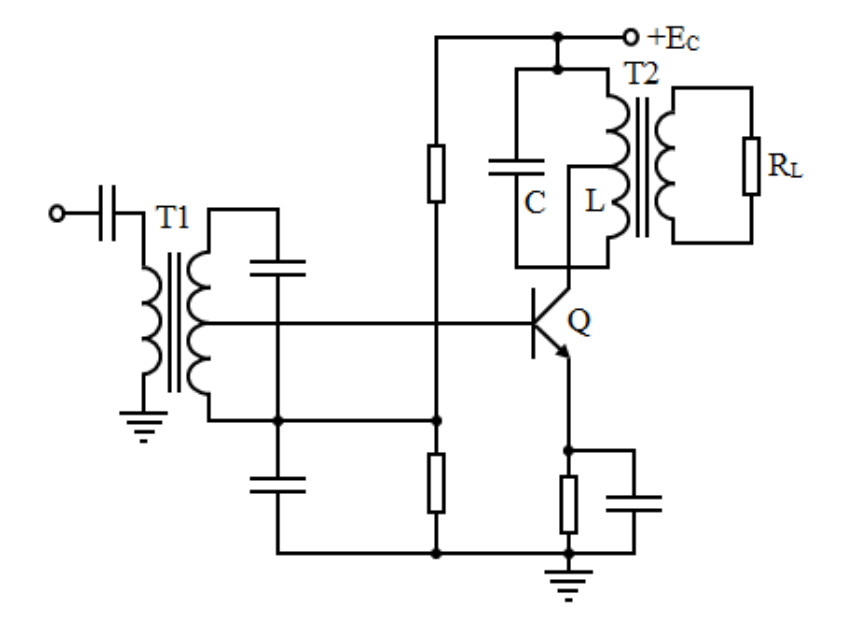
\includegraphics[width=\textwidth]{pics/mono_harmo_amplifier.png}
        \caption{单调谐放大器电路}\label{subfig:mono_harmo_amplifier}
    \end{subfigure}
    \begin{subfigure}[t]{0.45\textwidth}
        \centering
        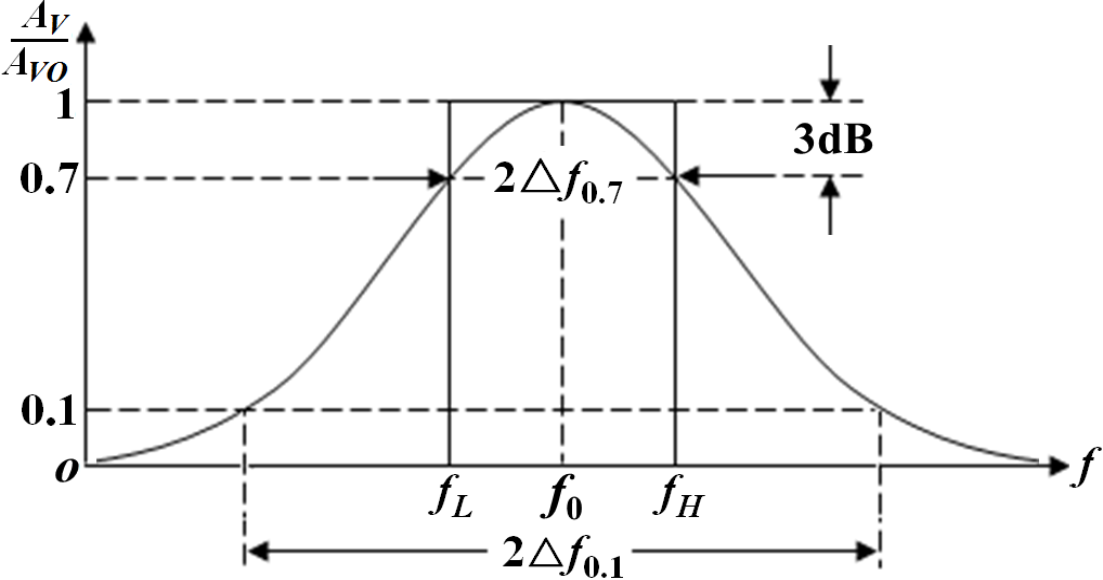
\includegraphics[width=\textwidth]{pics/mono_amp_f_characteristics.png}\caption{单调谐放大器幅频特性曲线}\label{subfig:mono_amp_f_characteristics}
    \end{subfigure}
    \caption{单调谐放大器}\label{fig:mono_harmo_amplifier}
\end{figure}

典型的双调谐放大器电路如图 \ref{subfig:bi_harmo_amplifier} 所示,集电极负载改为两个相互耦合的谐振回路,目的是改善矩形系数,提高选频能力。双调谐放大器幅频特性曲线如图 \ref{subfig:bi_amp_f_characteristics} 所示。

根据耦合程度不同,双调谐放大器可以分为弱耦合、临界耦合和强耦合。
弱耦合谐振曲线为单峰,通频带较窄,类似单调谐。临界耦合谐振曲线仍为单峰, 但顶部平坦
强耦合谐振曲线为双峰,中心频率处出现谷点,一般峰谷不低于-3dB。

\begin{figure}[H]
    \centering
    \begin{subfigure}[c]{0.45\textwidth}
        \centering
        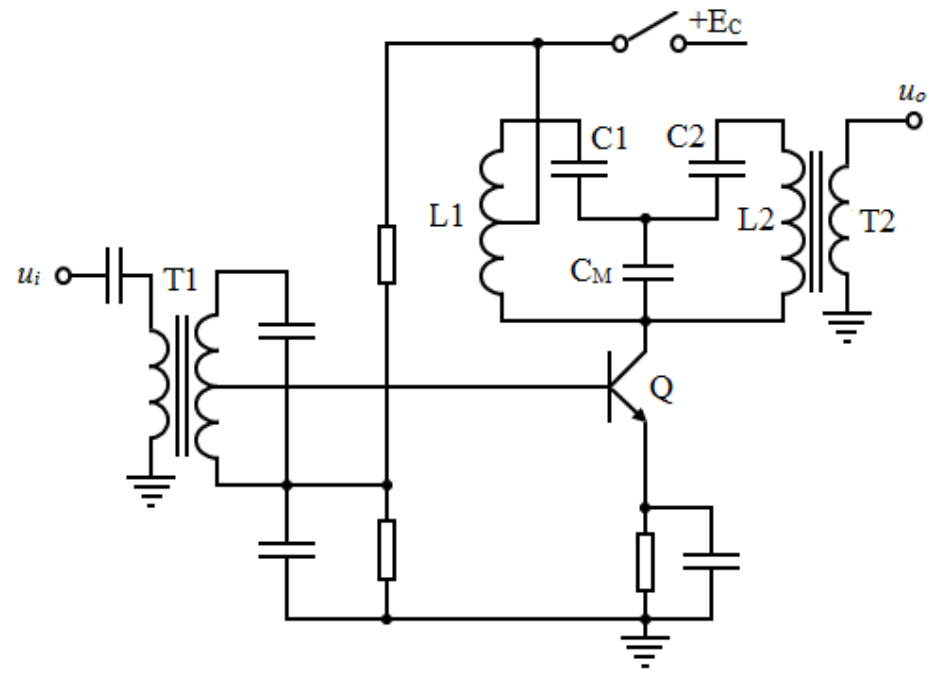
\includegraphics[width=0.9\textwidth]{pics/bi_harmo_amplifier.png}
        \caption{双调谐放大电路}\label{subfig:bi_harmo_amplifier}
    \end{subfigure}
    \begin{subfigure}[c]{0.45\textwidth}
        \centering
        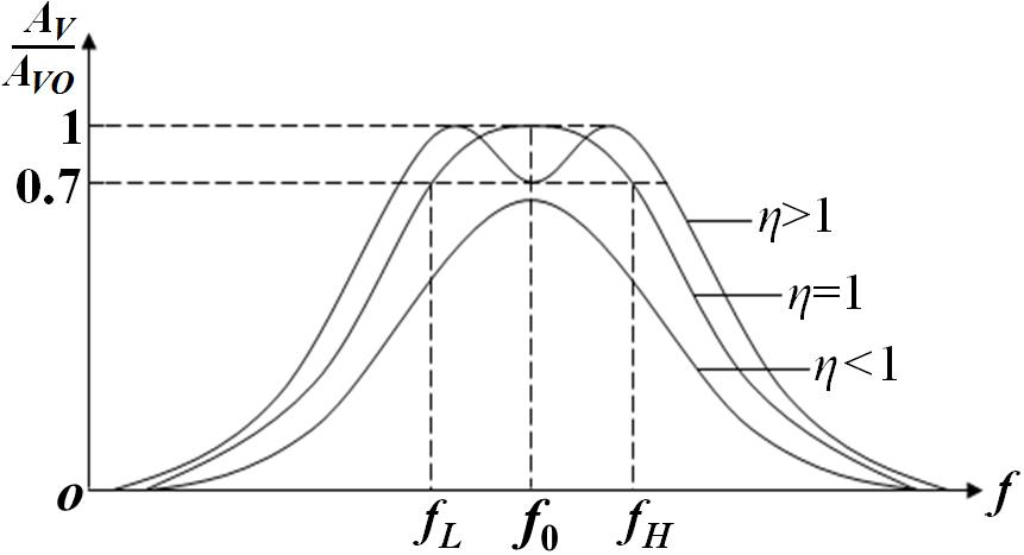
\includegraphics[width=0.9\textwidth]{pics/bi_amp_f_characteristics.png}
        \caption{双调谐放大幅频特性曲线}\label{subfig:bi_amp_f_characteristics}
    \end{subfigure}
    \caption{双调谐放大器}\label{fig:bi_harmo_amplifier}
\end{figure}

实验电路图如图\ref{fig:exp_circuit}所示,当JK2闭合时,C18被短路,电路为单调谐放大器实验电路。当JK2断开时,C18为耦合电容,为双调谐放大器实验电路。
\begin{figure}[H]
    \centering
    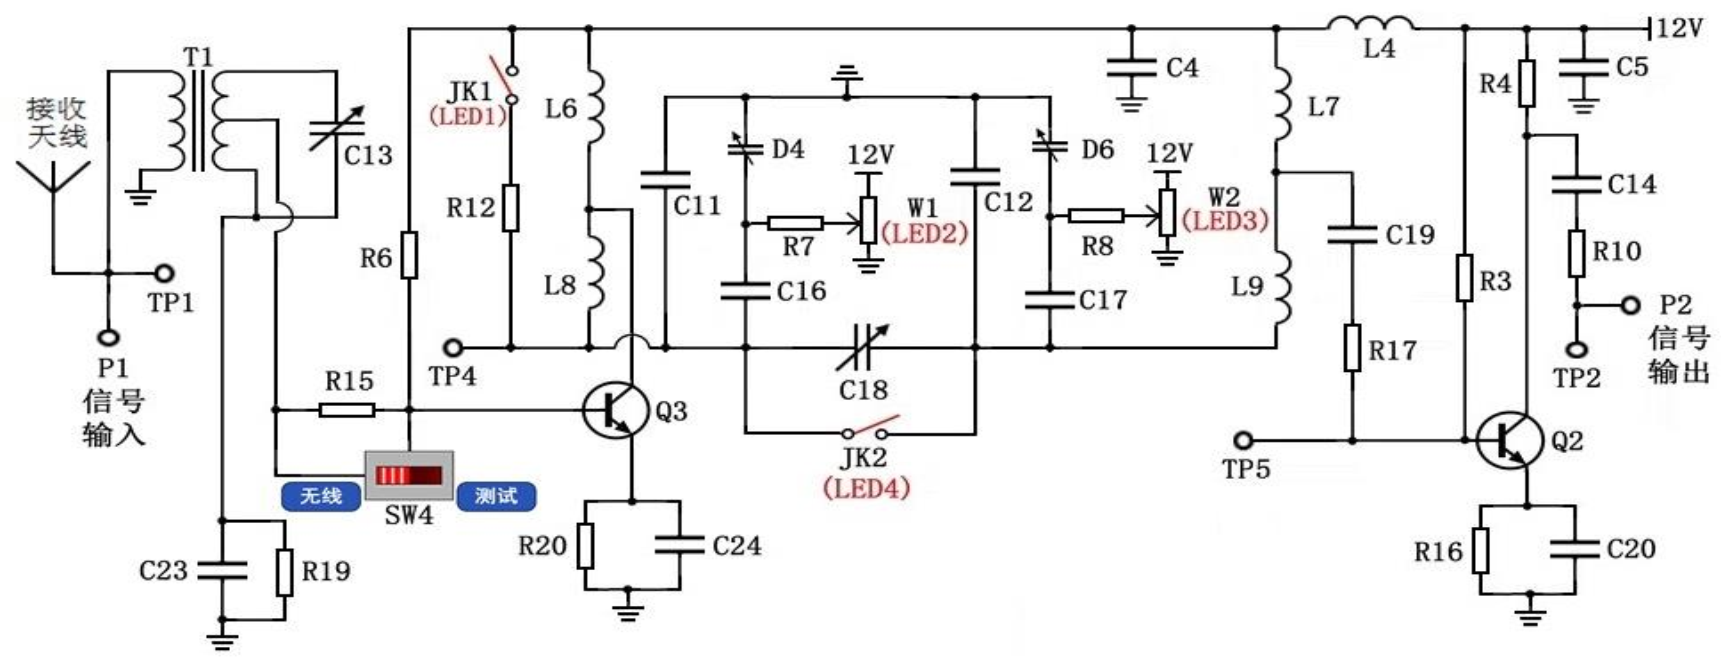
\includegraphics[width=0.9\textwidth]{pics/exp_circuit.png}
    \caption{实验电路图}\label{fig:exp_circuit}
\end{figure}




\section{第三部分 \texorpdfstring{\quad}{} 实验内容及结果}
\subsection{单调谐放大器频域测量}
\begin{enumerate}[(1)]
    \item \noindent \textbf{单调谐放大器幅频特性曲线以及对应中心频率(10.7 MHz)的幅值}
    \begin{figure}[H]
        \centering
        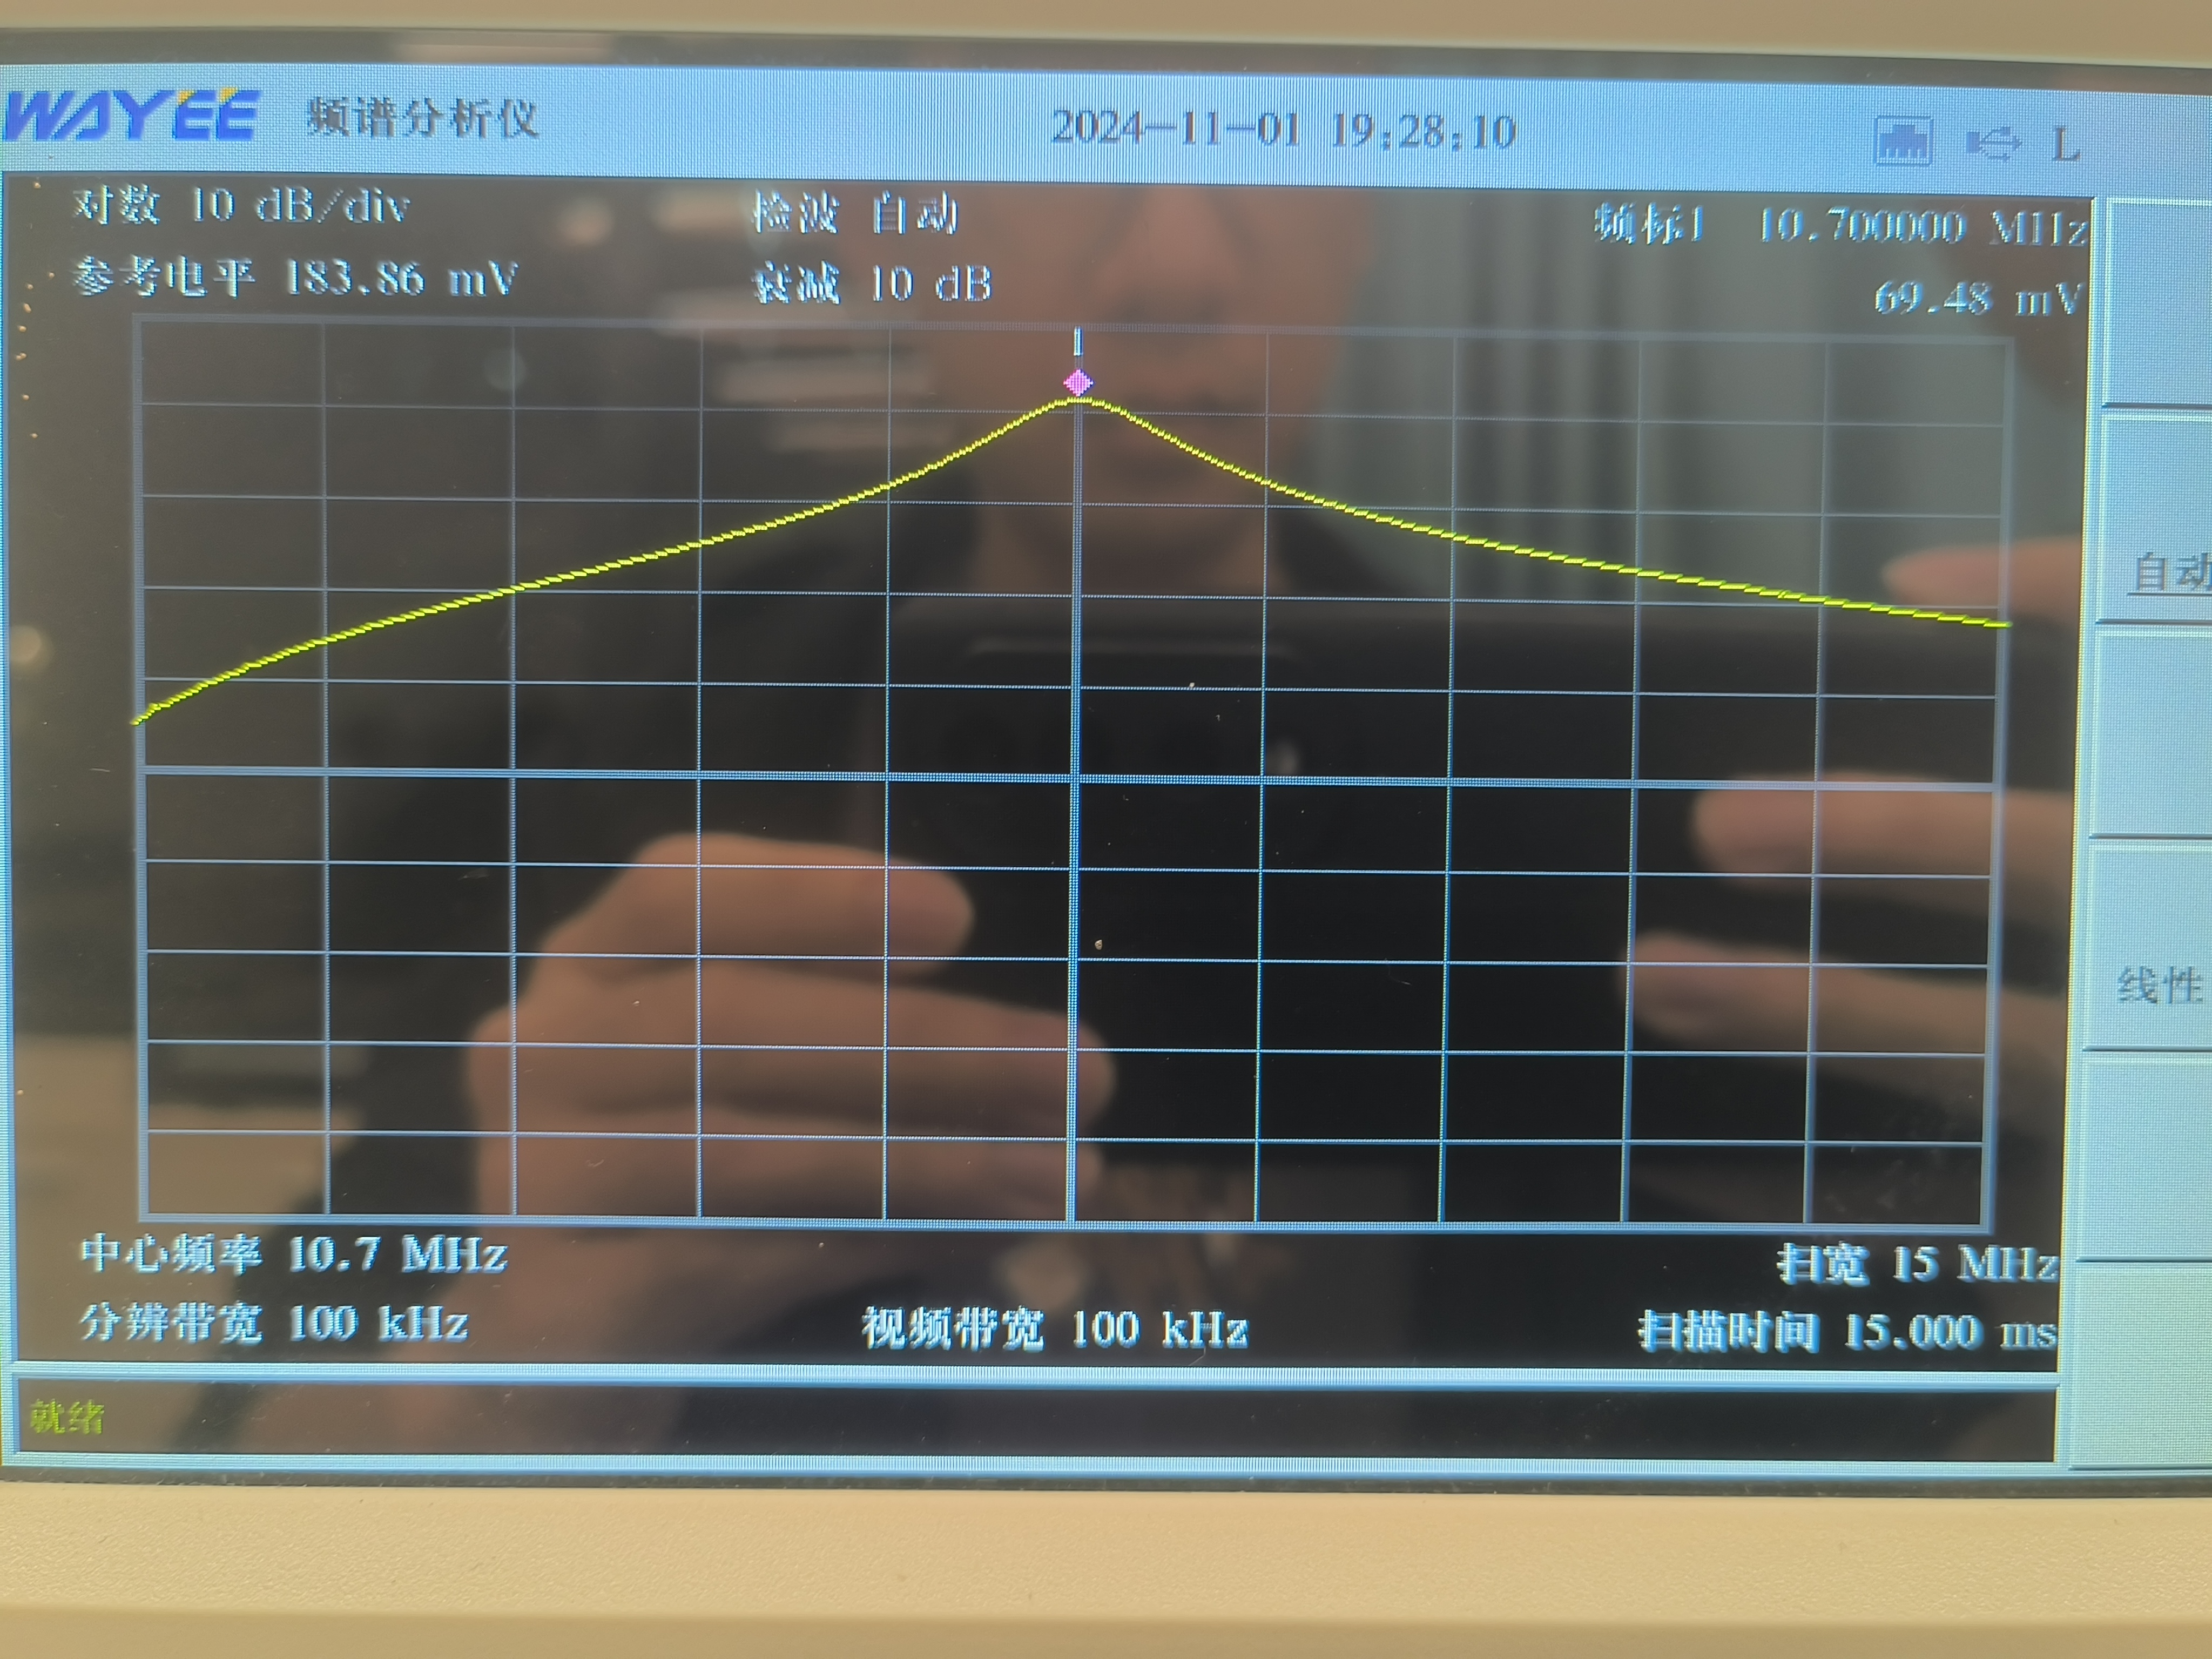
\includegraphics[width=0.5\textwidth]{pics/3.1.1.png}
        ~\\
        \caption{单调谐放大器幅频特性曲线}\label{fig:3.1.1}
    \end{figure}

    由图\ref{fig:3.1.1}中可以得到中心频率幅值为$69.48mV$。
    
    \item \noindent \textbf{单调谐放大器$N(3)dB$ 带宽 $N(20)dB$ 带宽与矩形系数}
    
    测量得单调谐放大器$N(3)dB$带宽为
    $2\Delta f_{0.7}=1.15MHz$,$N(20)dB$带宽为
    $2\Delta f_{0.1}=9.675MHz$

    计算得到矩形系数为
    $K_{r0.1}=\dfrac{2\Delta f_{0.1}}{2\Delta f_{0.7}}=8.413$
    
    \item \noindent \textbf{单调谐放大器谐振电压增益 $A_{VO}$}    
    \begin{figure}[H]
        \centering
        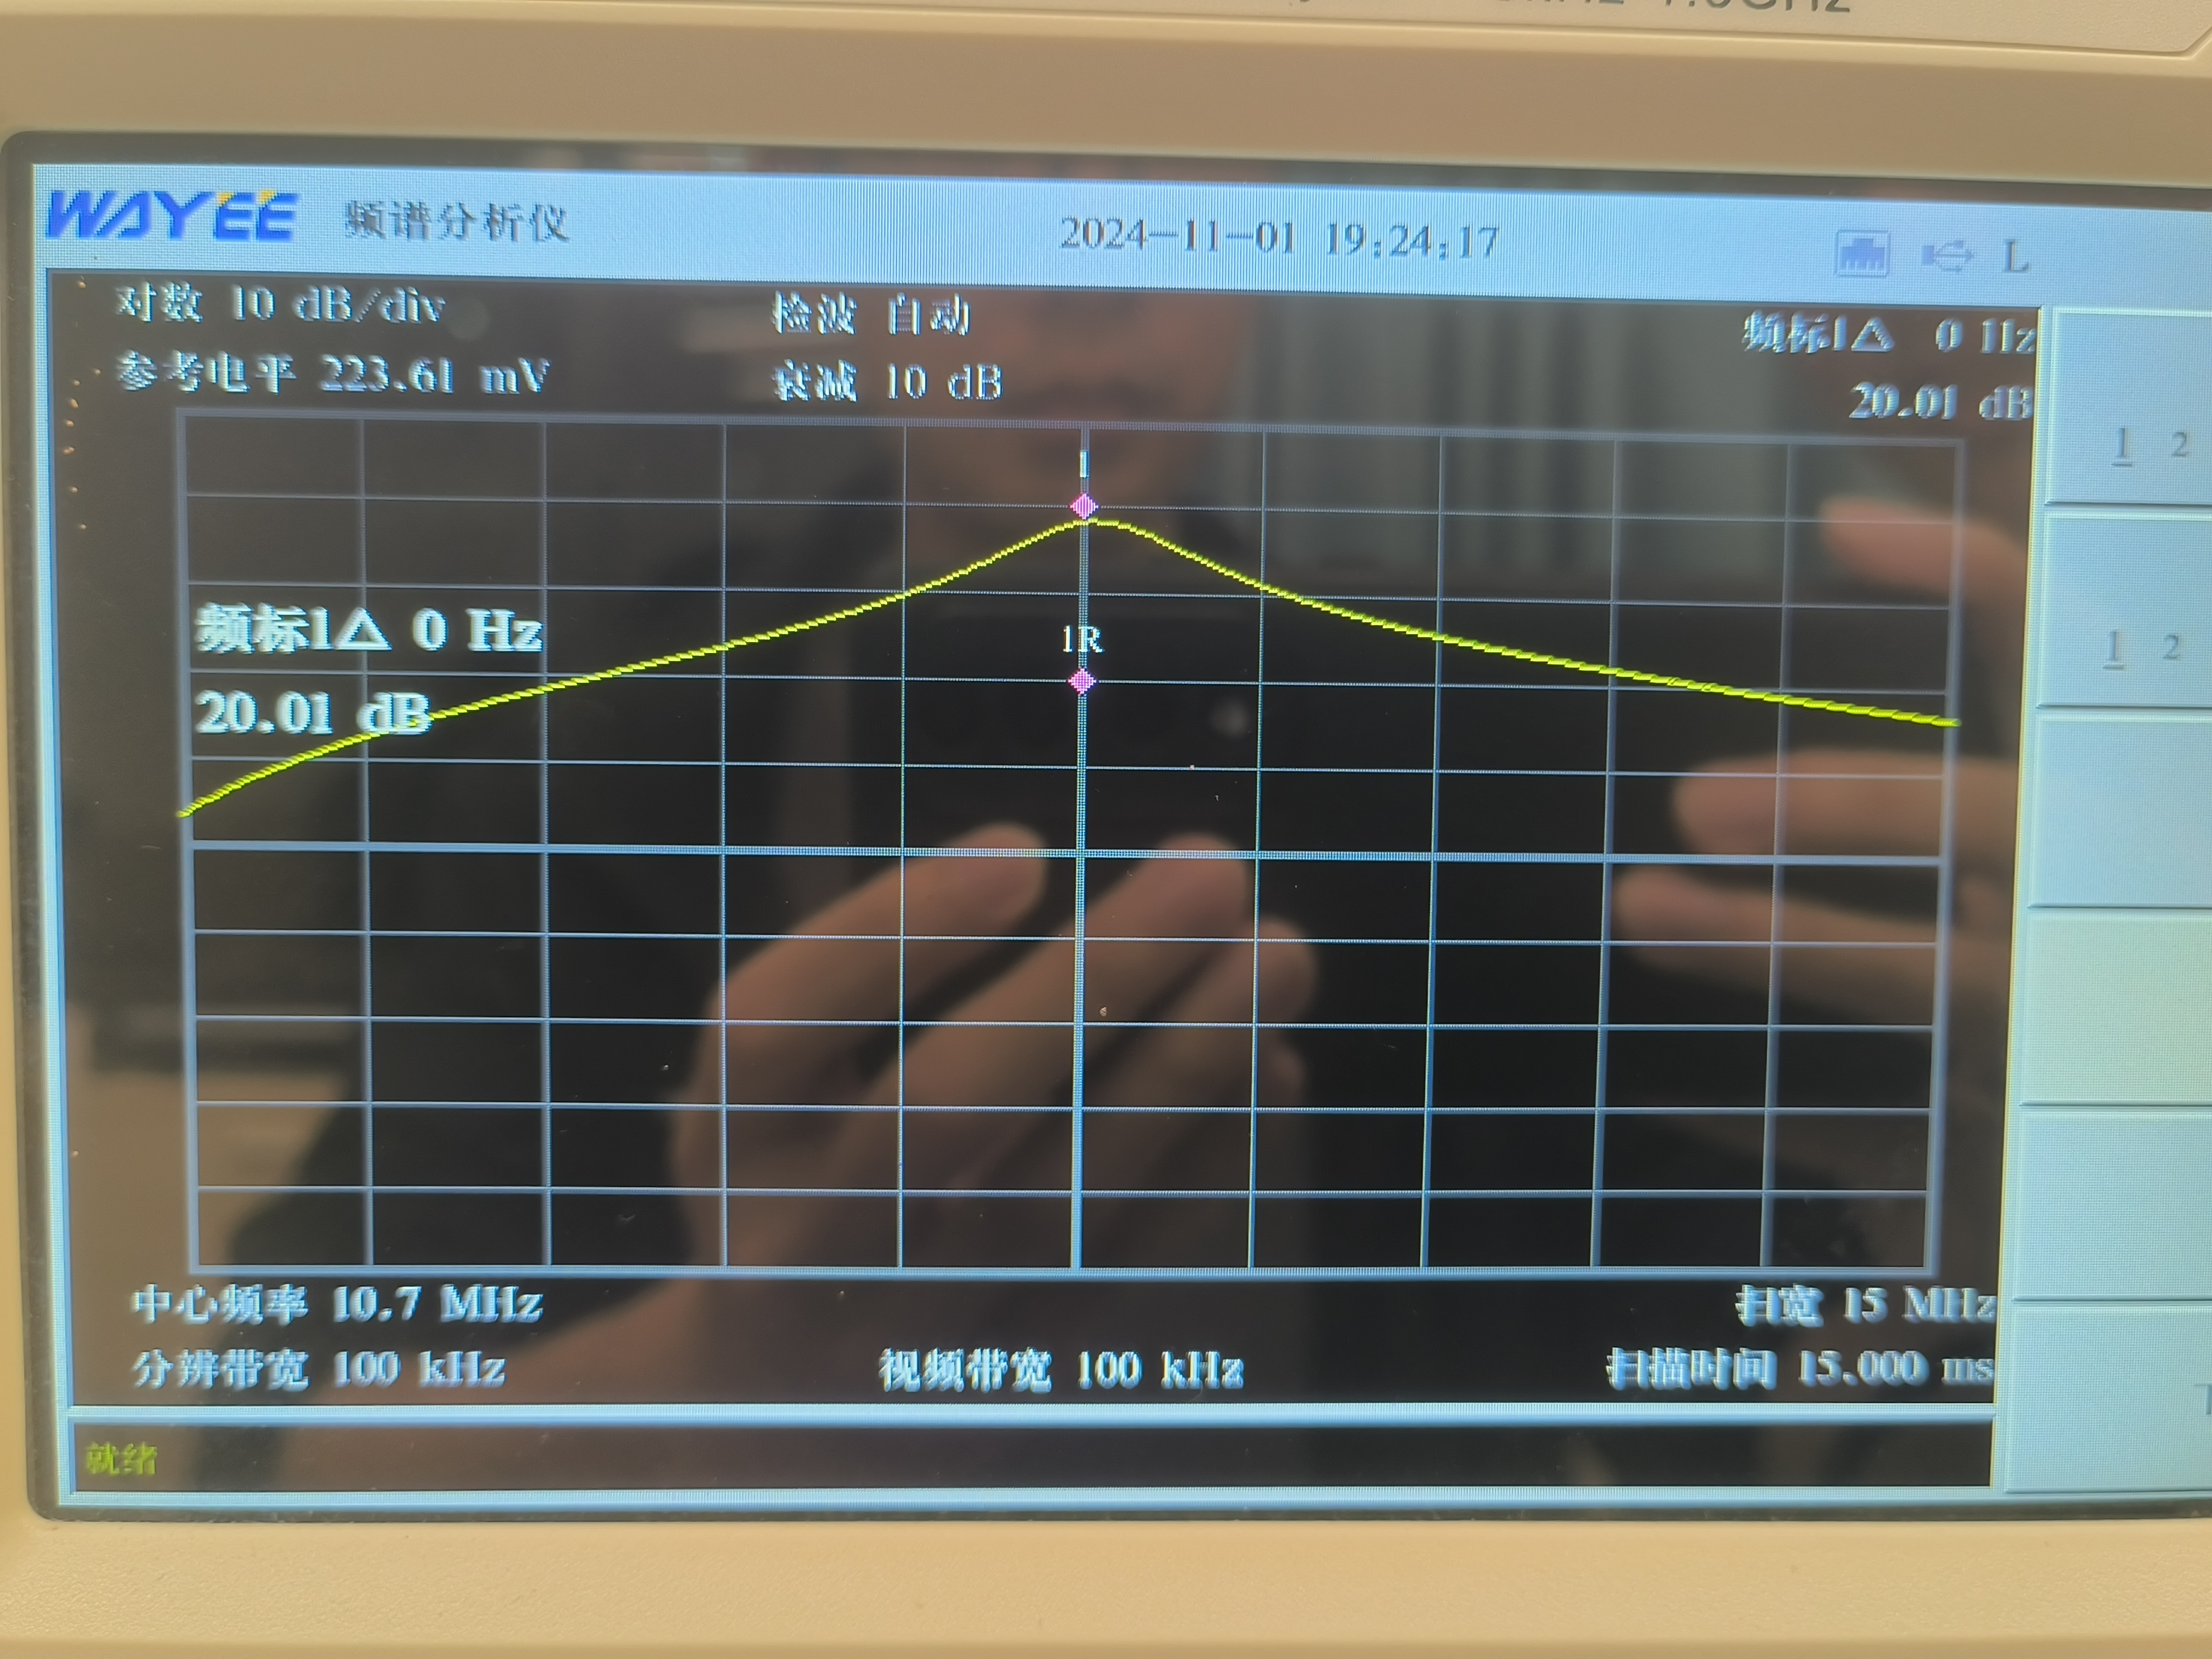
\includegraphics[width=0.5\textwidth]{pics/3.1.3.png}
        ~\\
        \caption{单调谐放大器谐振电压增益线}\label{fig:3.1.3}
    \end{figure}

    由图\ref{fig:3.1.3}中可以读出单调谐放大器谐振电压增益 $A_{VO}=20.01dB$

    如果考虑频谱仪上标注的衰减10dB,此时实际电压增益应为$A_{VO}=30.01dB$
    
    \item \noindent \textbf{接入阻尼电阻后,单调谐放大器幅频特性曲线以及对应中心频率(10.7 MHz)的幅值}    
    \begin{figure}[H]
        \centering
        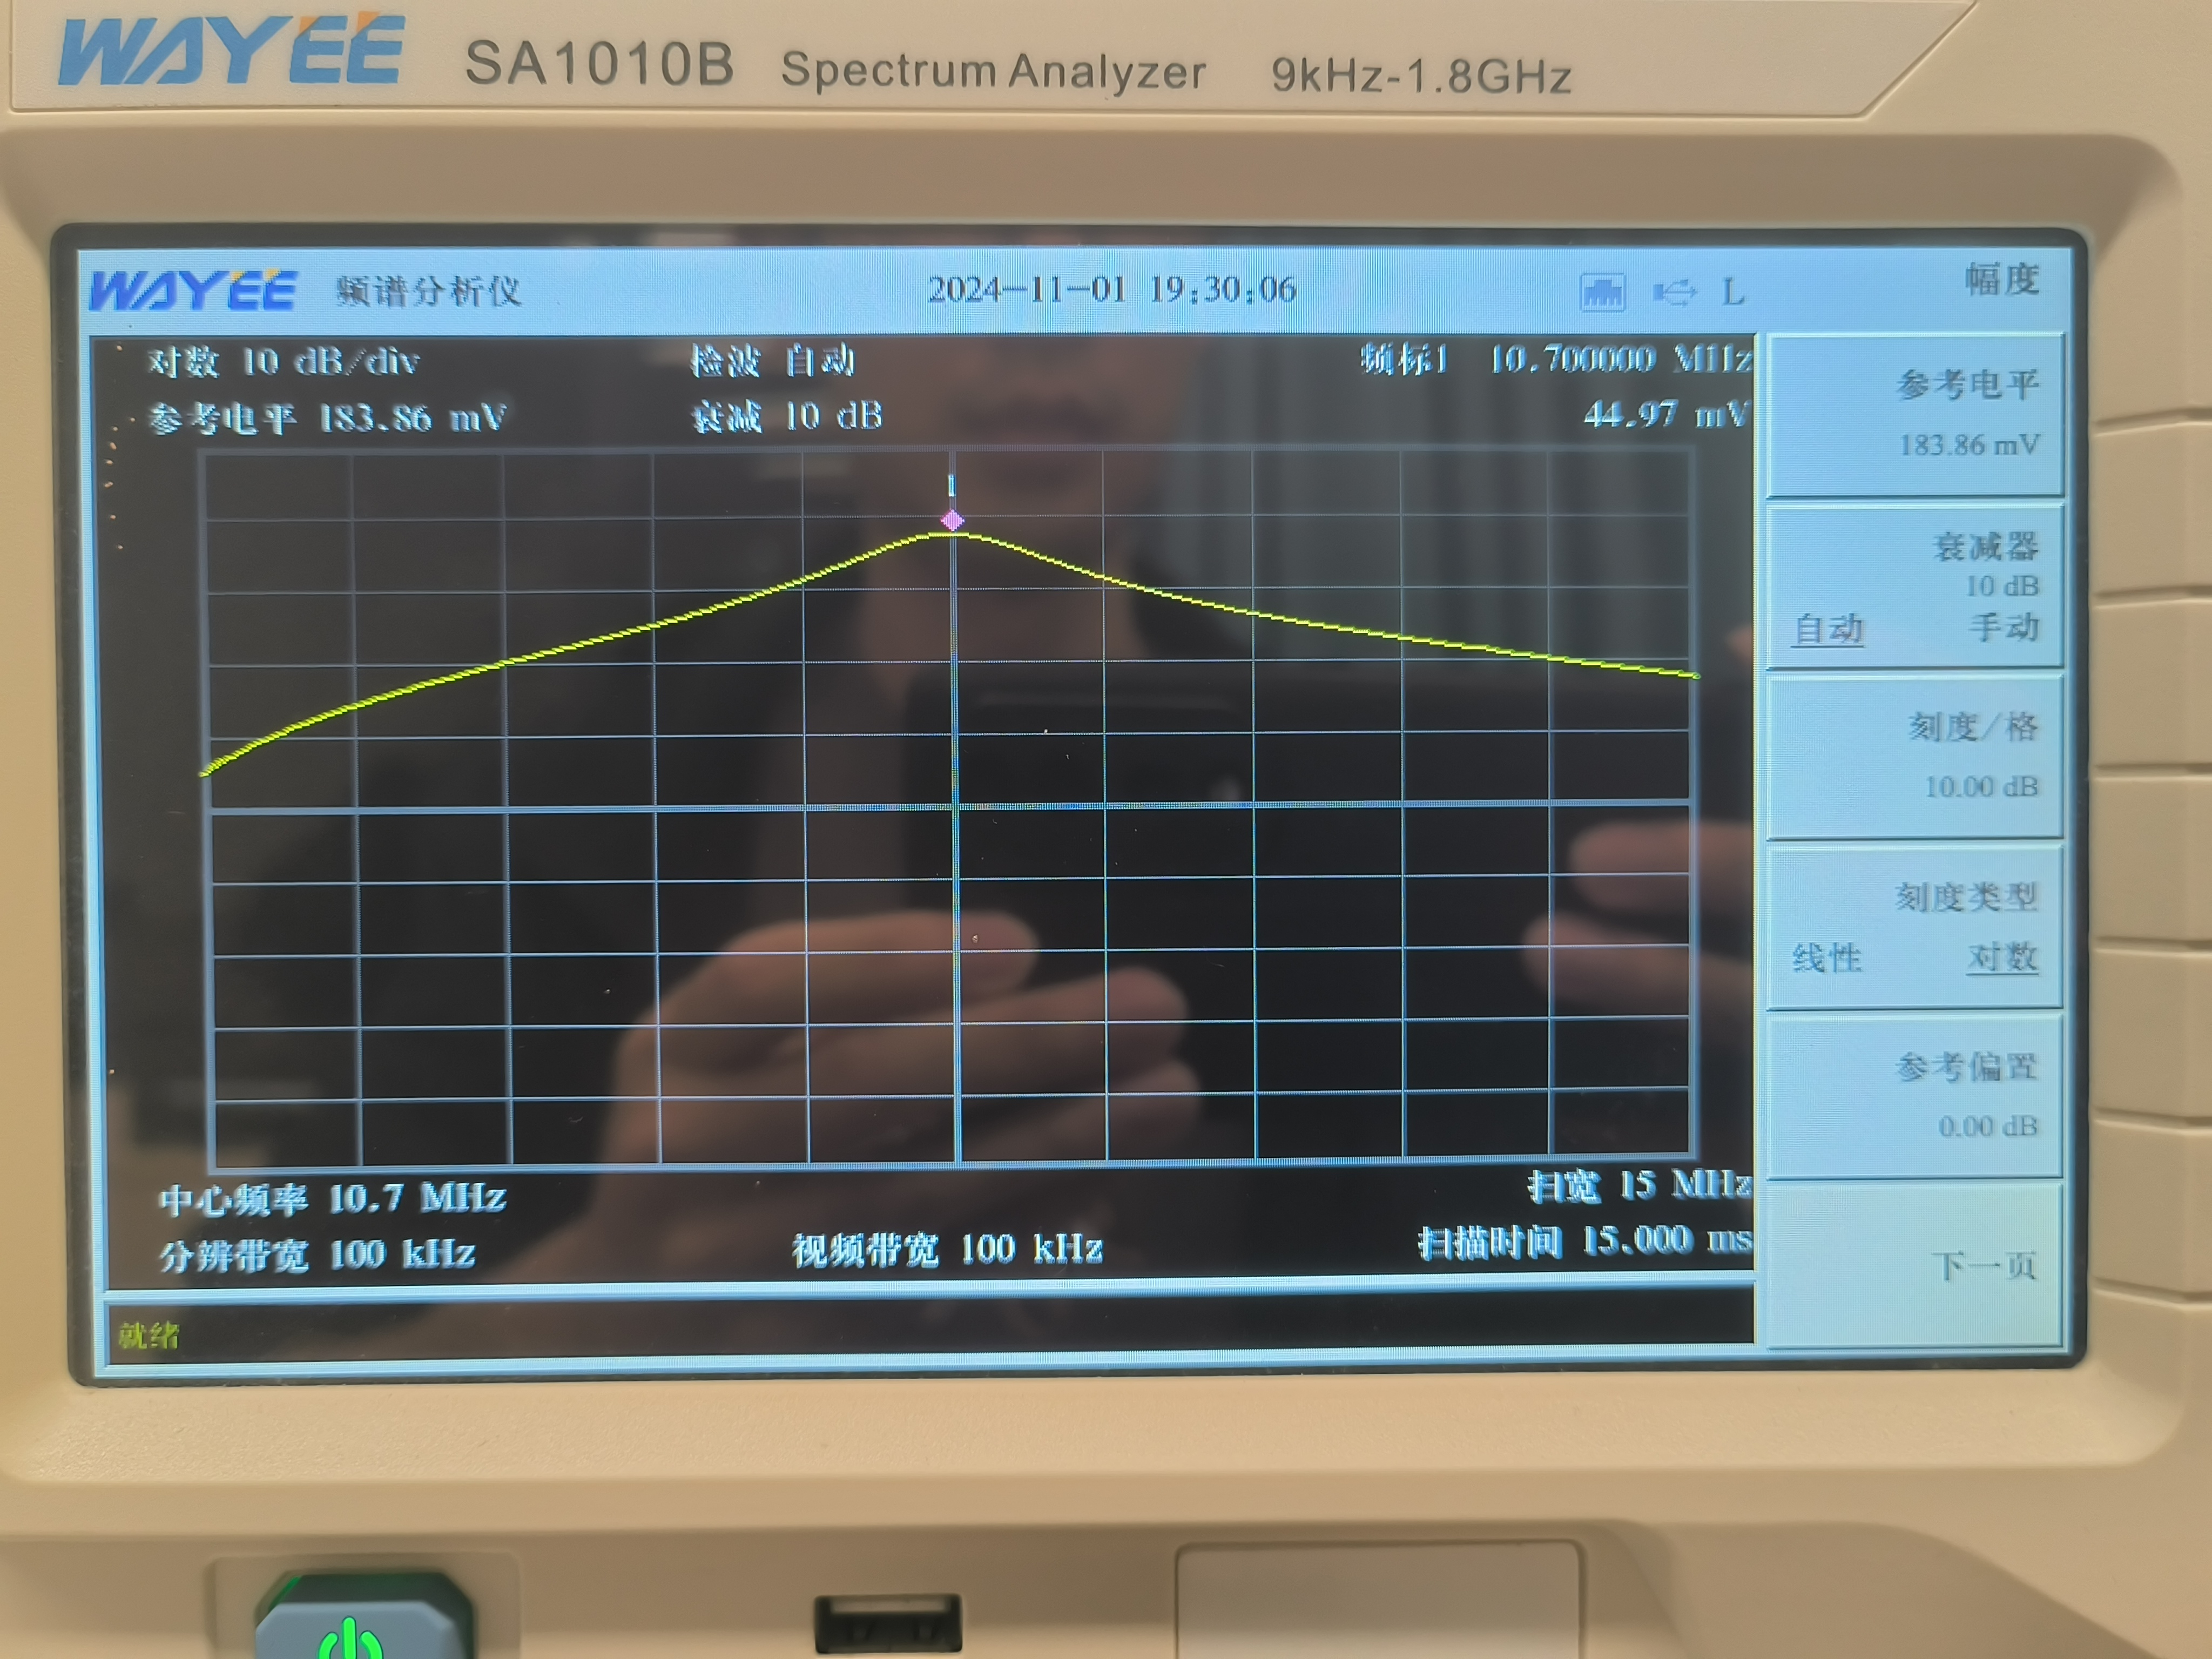
\includegraphics[width=0.5\textwidth]{pics/3.1.4.png}
        ~\\
        \caption{接入阻尼电阻后的单调谐放大器幅频特性曲线}\label{fig:3.1.4}
    \end{figure}

    由图\ref{fig:3.1.4}中可以读出接入阻尼电阻后单调谐放大器中心频率幅值为$44.97mV$。
  
    \item \noindent \textbf{接入阻尼电阻后,单调谐放大器$N(3)dB$ 带宽 $N(20)dB$ 带宽与矩形系数}

    测量得$N(3)dB$带宽为$2\Delta f_{0.7}=1.725MHz$,
    $N(20)dB$带宽为$2\Delta f_{0.1}=12.725MHz$

    计算得到矩形系数为
    $K_{r0.1}=\dfrac{2\Delta f_{0.1}}{2\Delta f_{0.7}}=7.377$
    
    \item \noindent \textbf{接入阻尼电阻后,单调谐放大器谐振电压增益 $A_{VO}$}
    \begin{figure}[H]
        \centering
        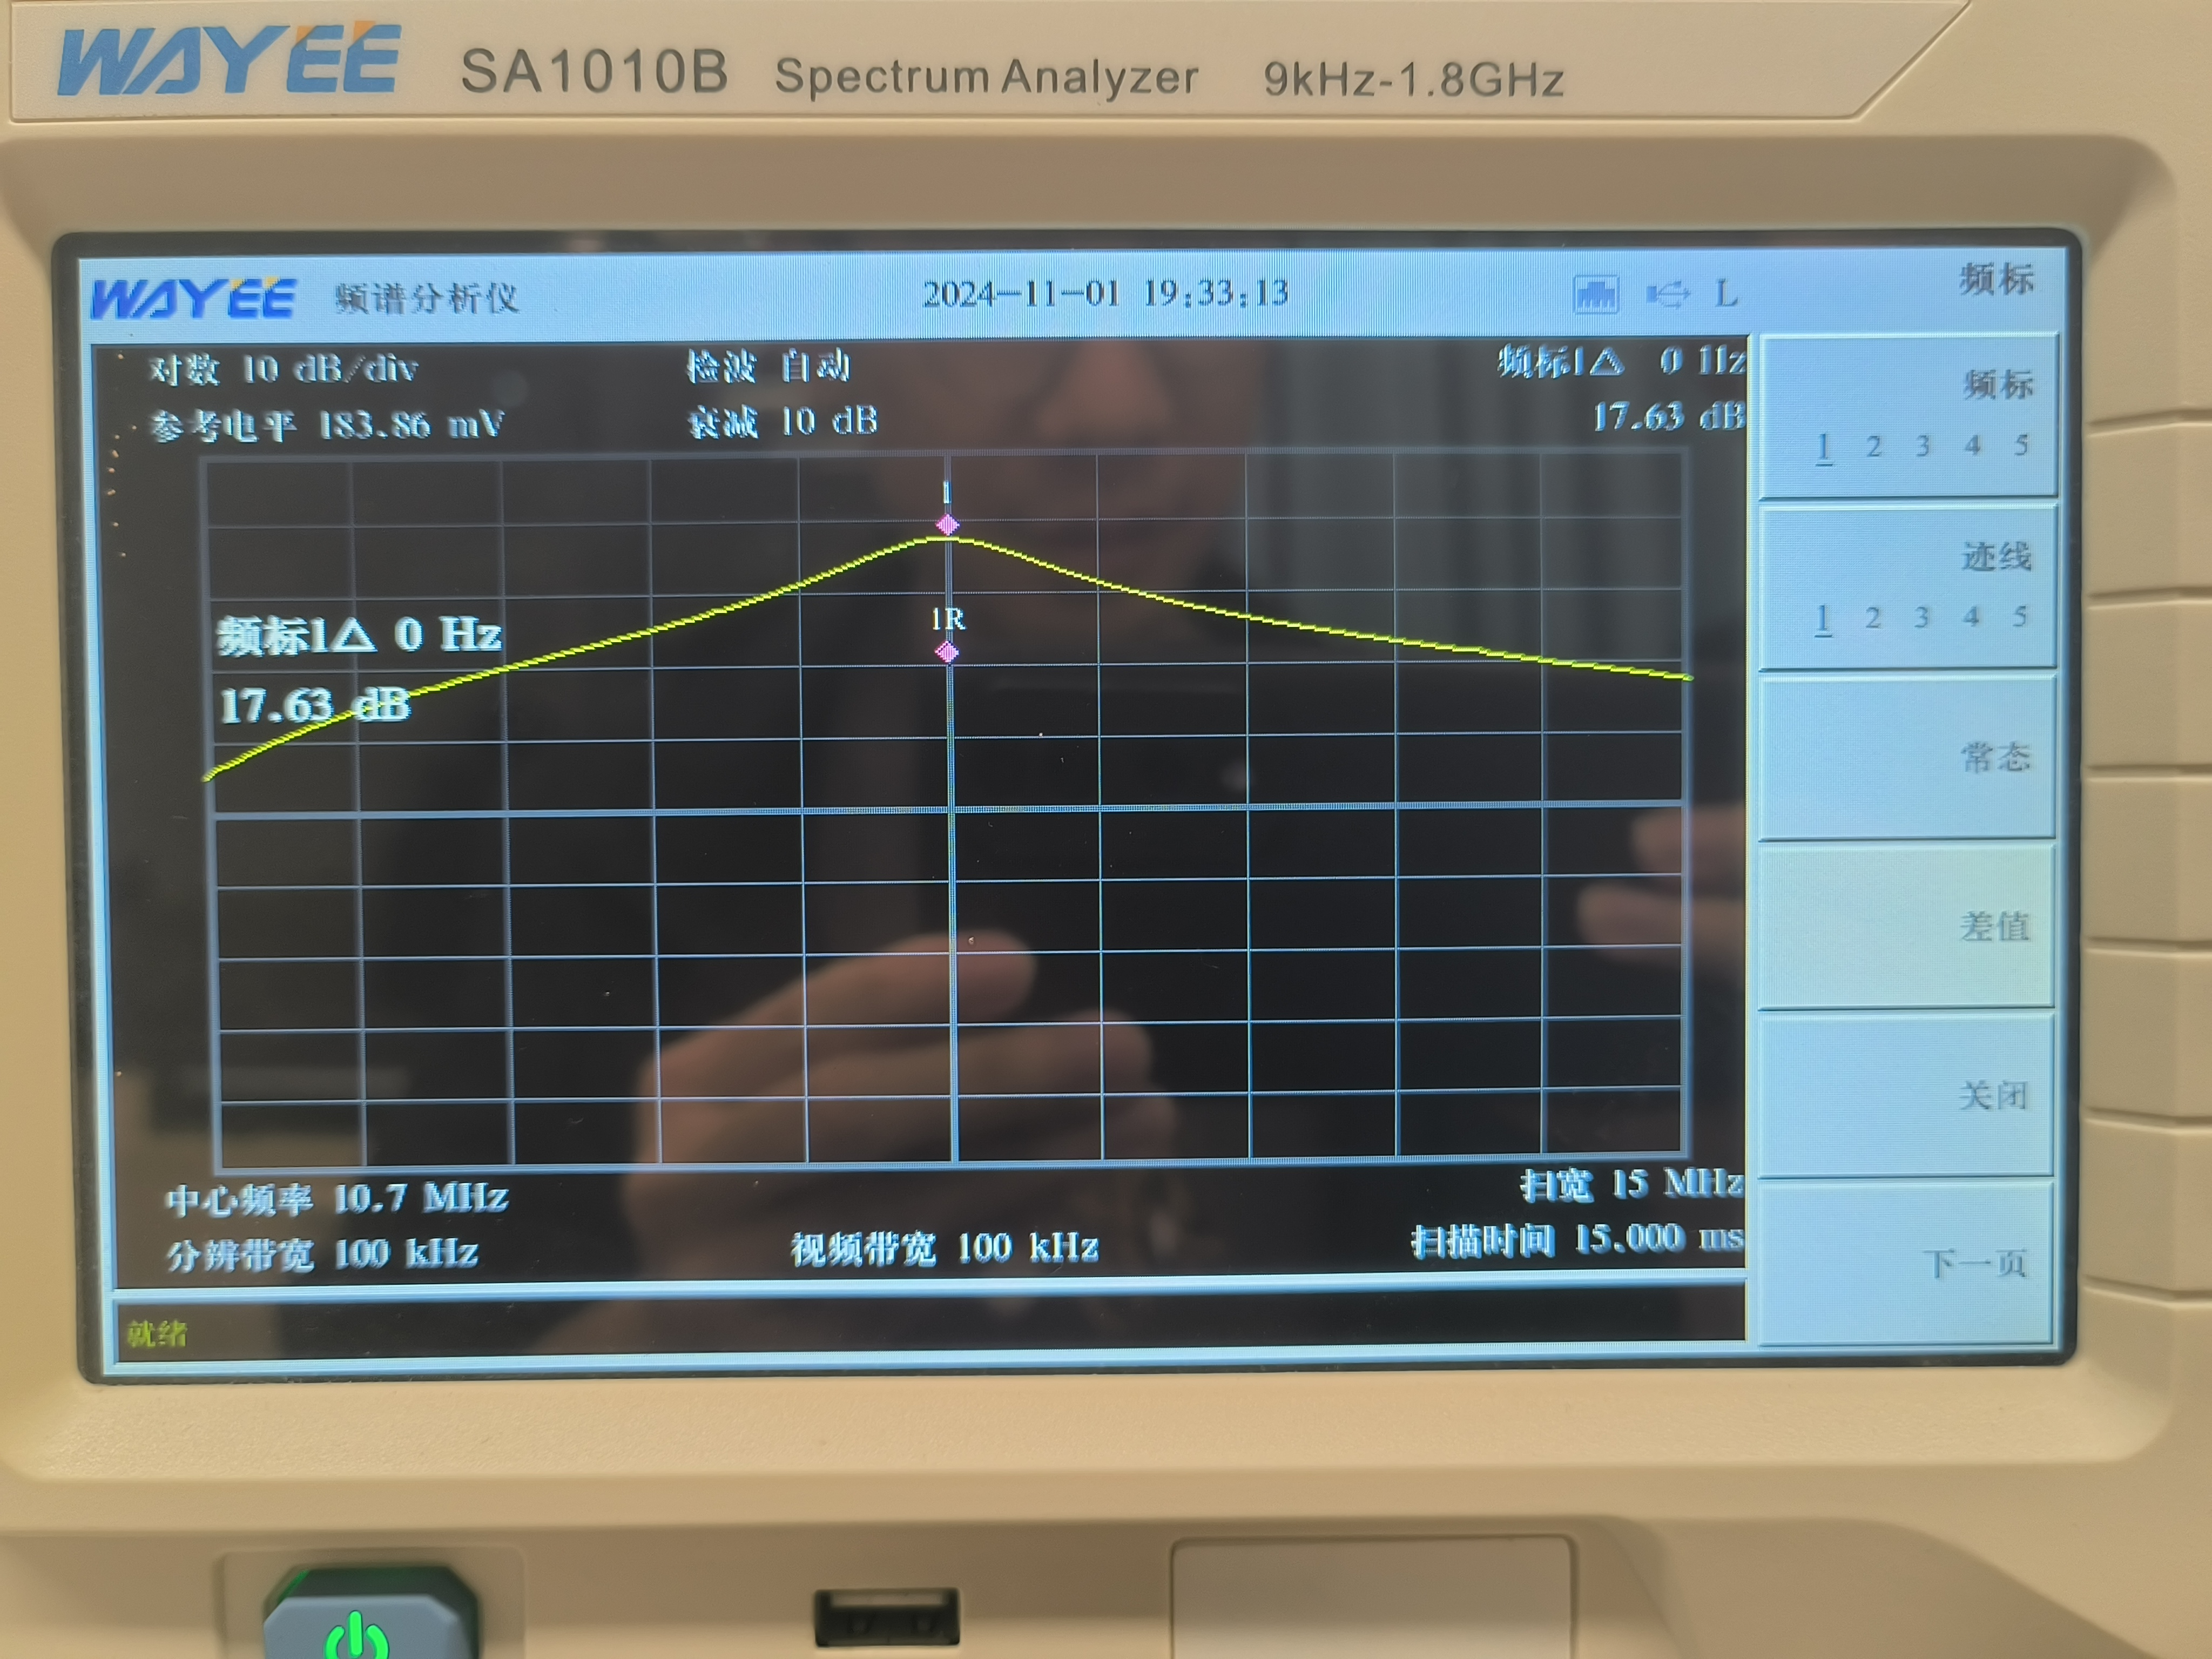
\includegraphics[width=0.5\textwidth]{pics/3.1.6.png}
        ~\\
        \caption{接入阻尼电阻后的单调谐放大器幅频特性曲线}\label{fig:3.1.6}
    \end{figure}

    \vspace{-2em}
    由图\ref{fig:3.1.6}中可以读出谐振电压增益$A_{VO}=17.63dB$
    
    如果考虑频谱仪上标注的衰减10dB,此时实际电压增益应为$A_{VO}=27.63dB$    
\end{enumerate}

\subsection{单调谐放大器时域测量}
\begin{enumerate}[(1)]
    \item \noindent\textbf{谐振电压增益 $A_{VO}$}
    
    \begin{figure}[H]
        \centering
        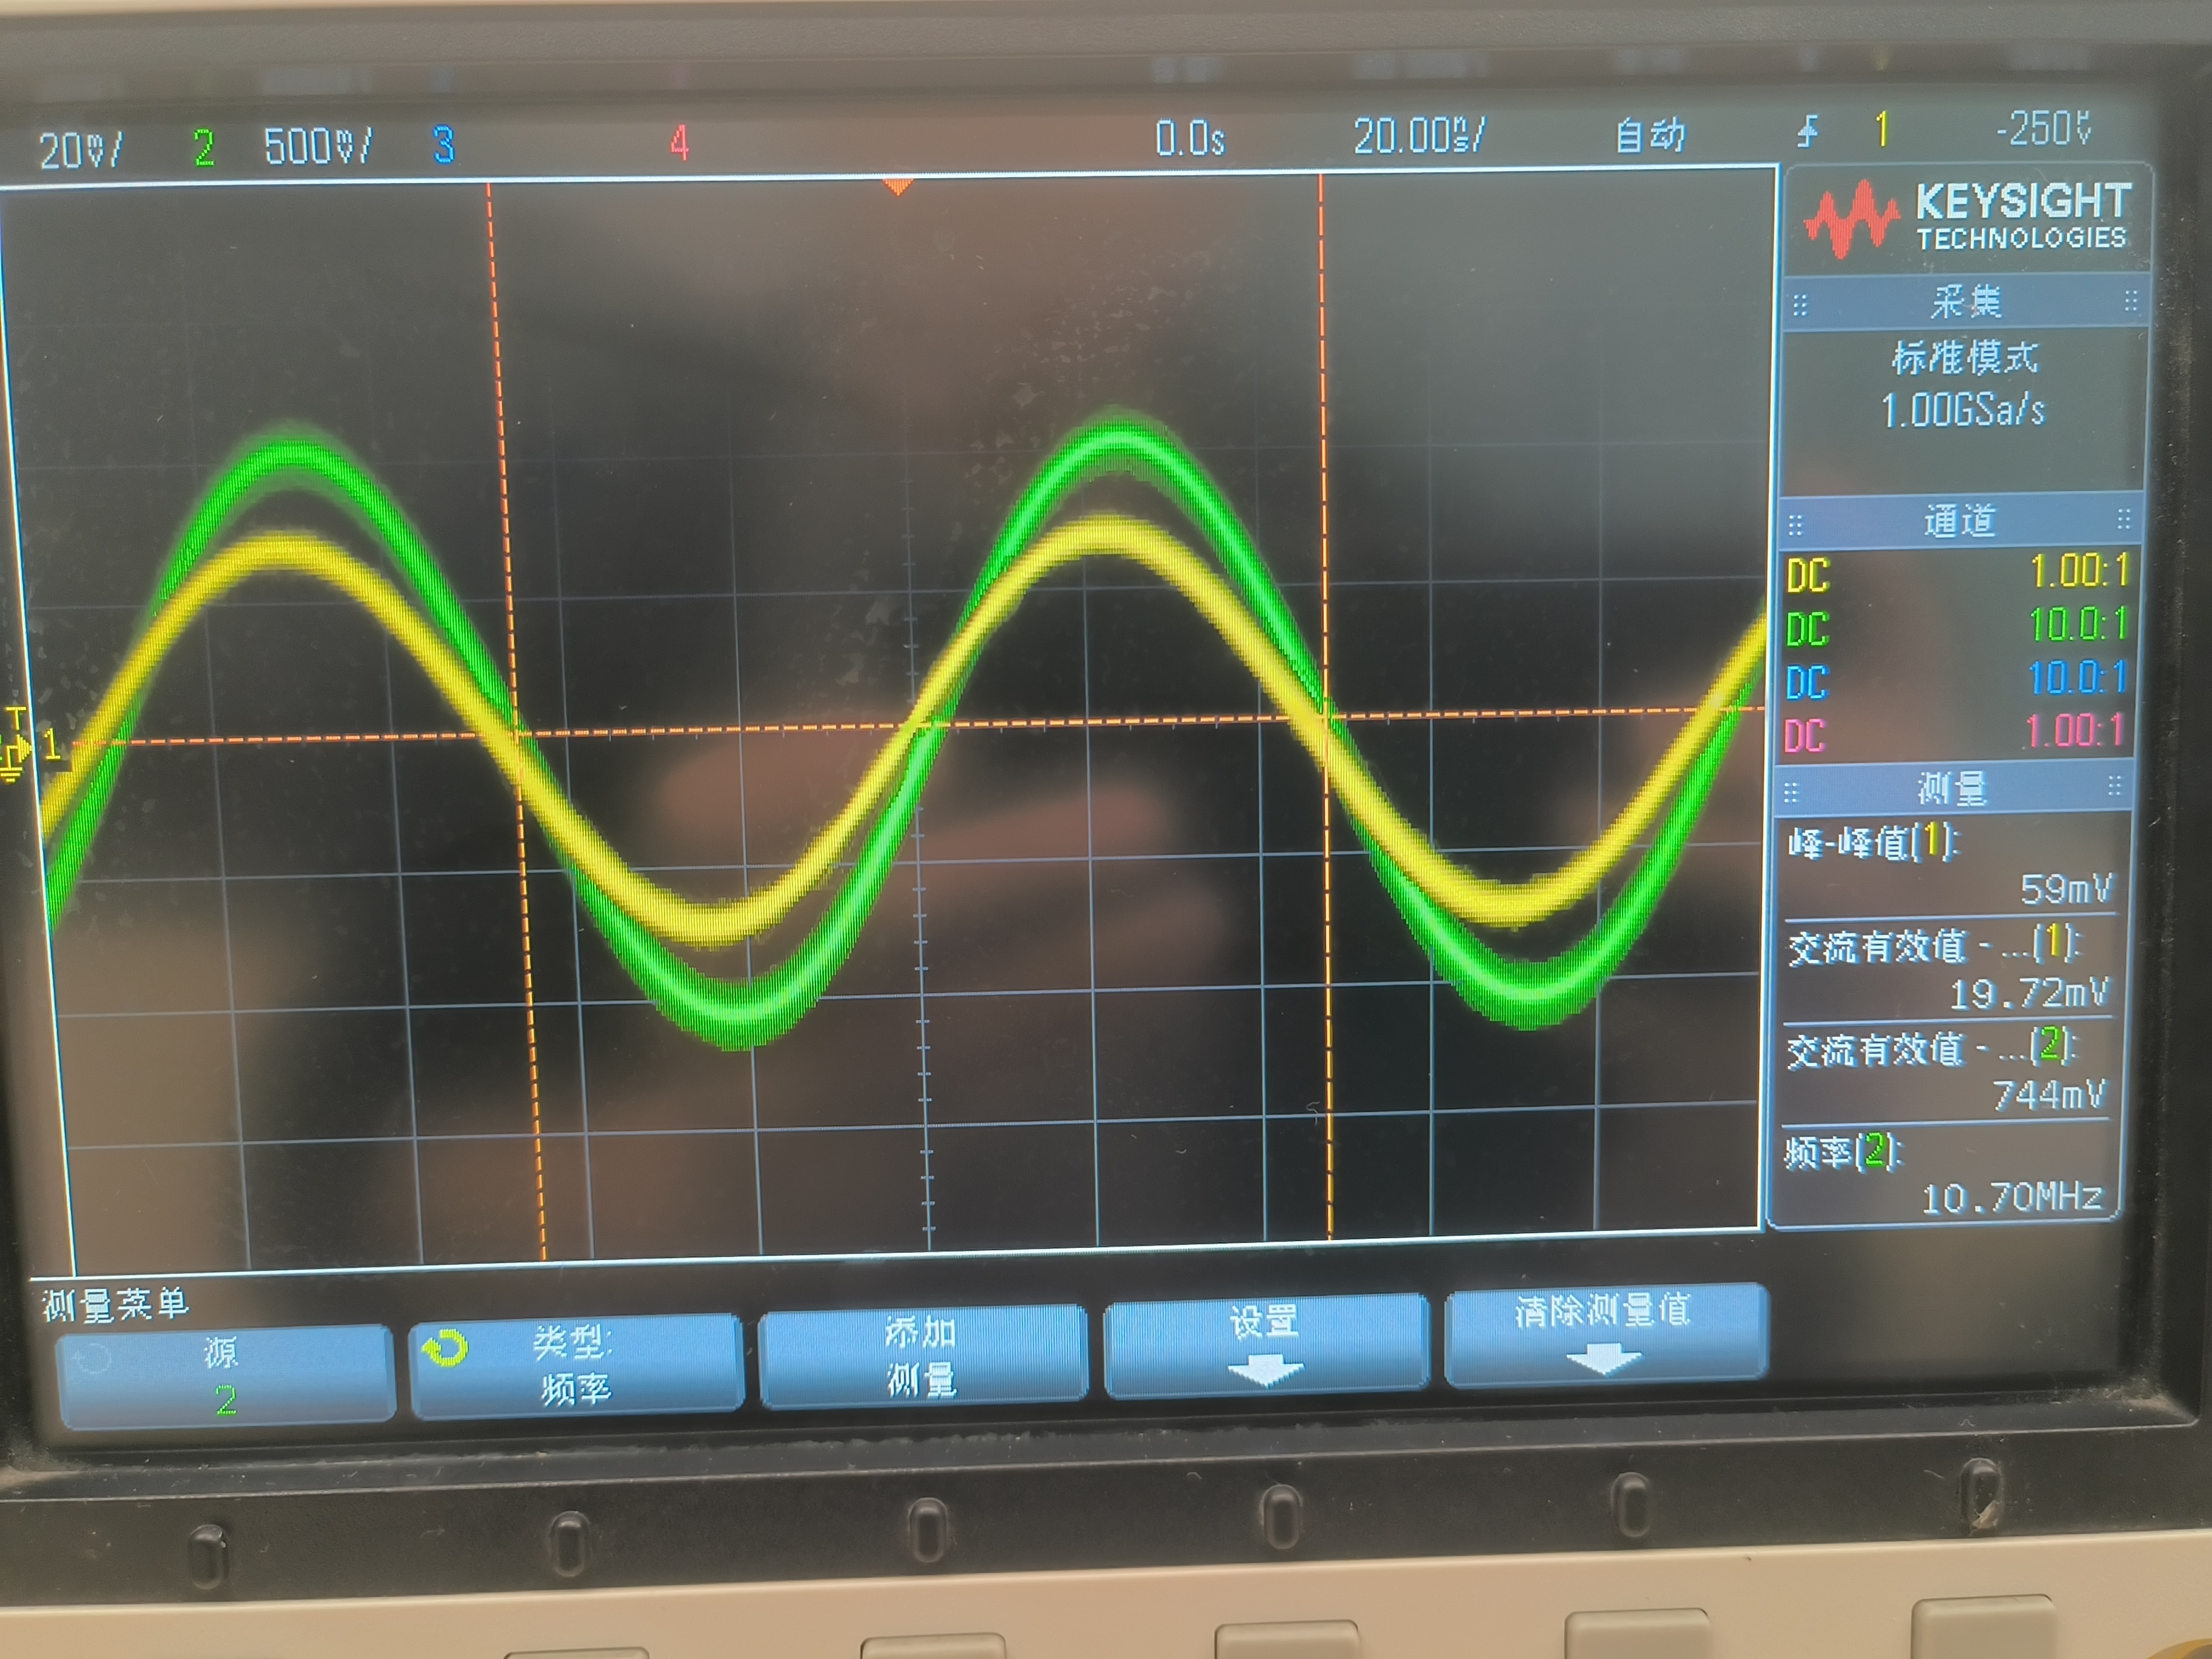
\includegraphics[width=0.45\textwidth]{pics/3.2.1.png}
        ~\\
        \caption{单调谐放大器时域输入输出波形}\label{fig:3.2.1}
    \end{figure}
    \vspace{-2em}
    输入有效值$U_i=19.72mV$,输出有效值$U_o=744mV$,
    谐振电压增益 $A_{VO}=\dfrac{U_o}{U_i}=37.73=31.53dB$

    与频域测得的电压增益30.01dB(考虑频谱仪衰减)相比较,误差在合理范围内。
    
    \item \noindent\textbf{$N(3)dB$ 通频带}
    
    \begin{figure}[H]
        \centering
        \begin{subfigure}[c]{0.45\textwidth}
            \centering
            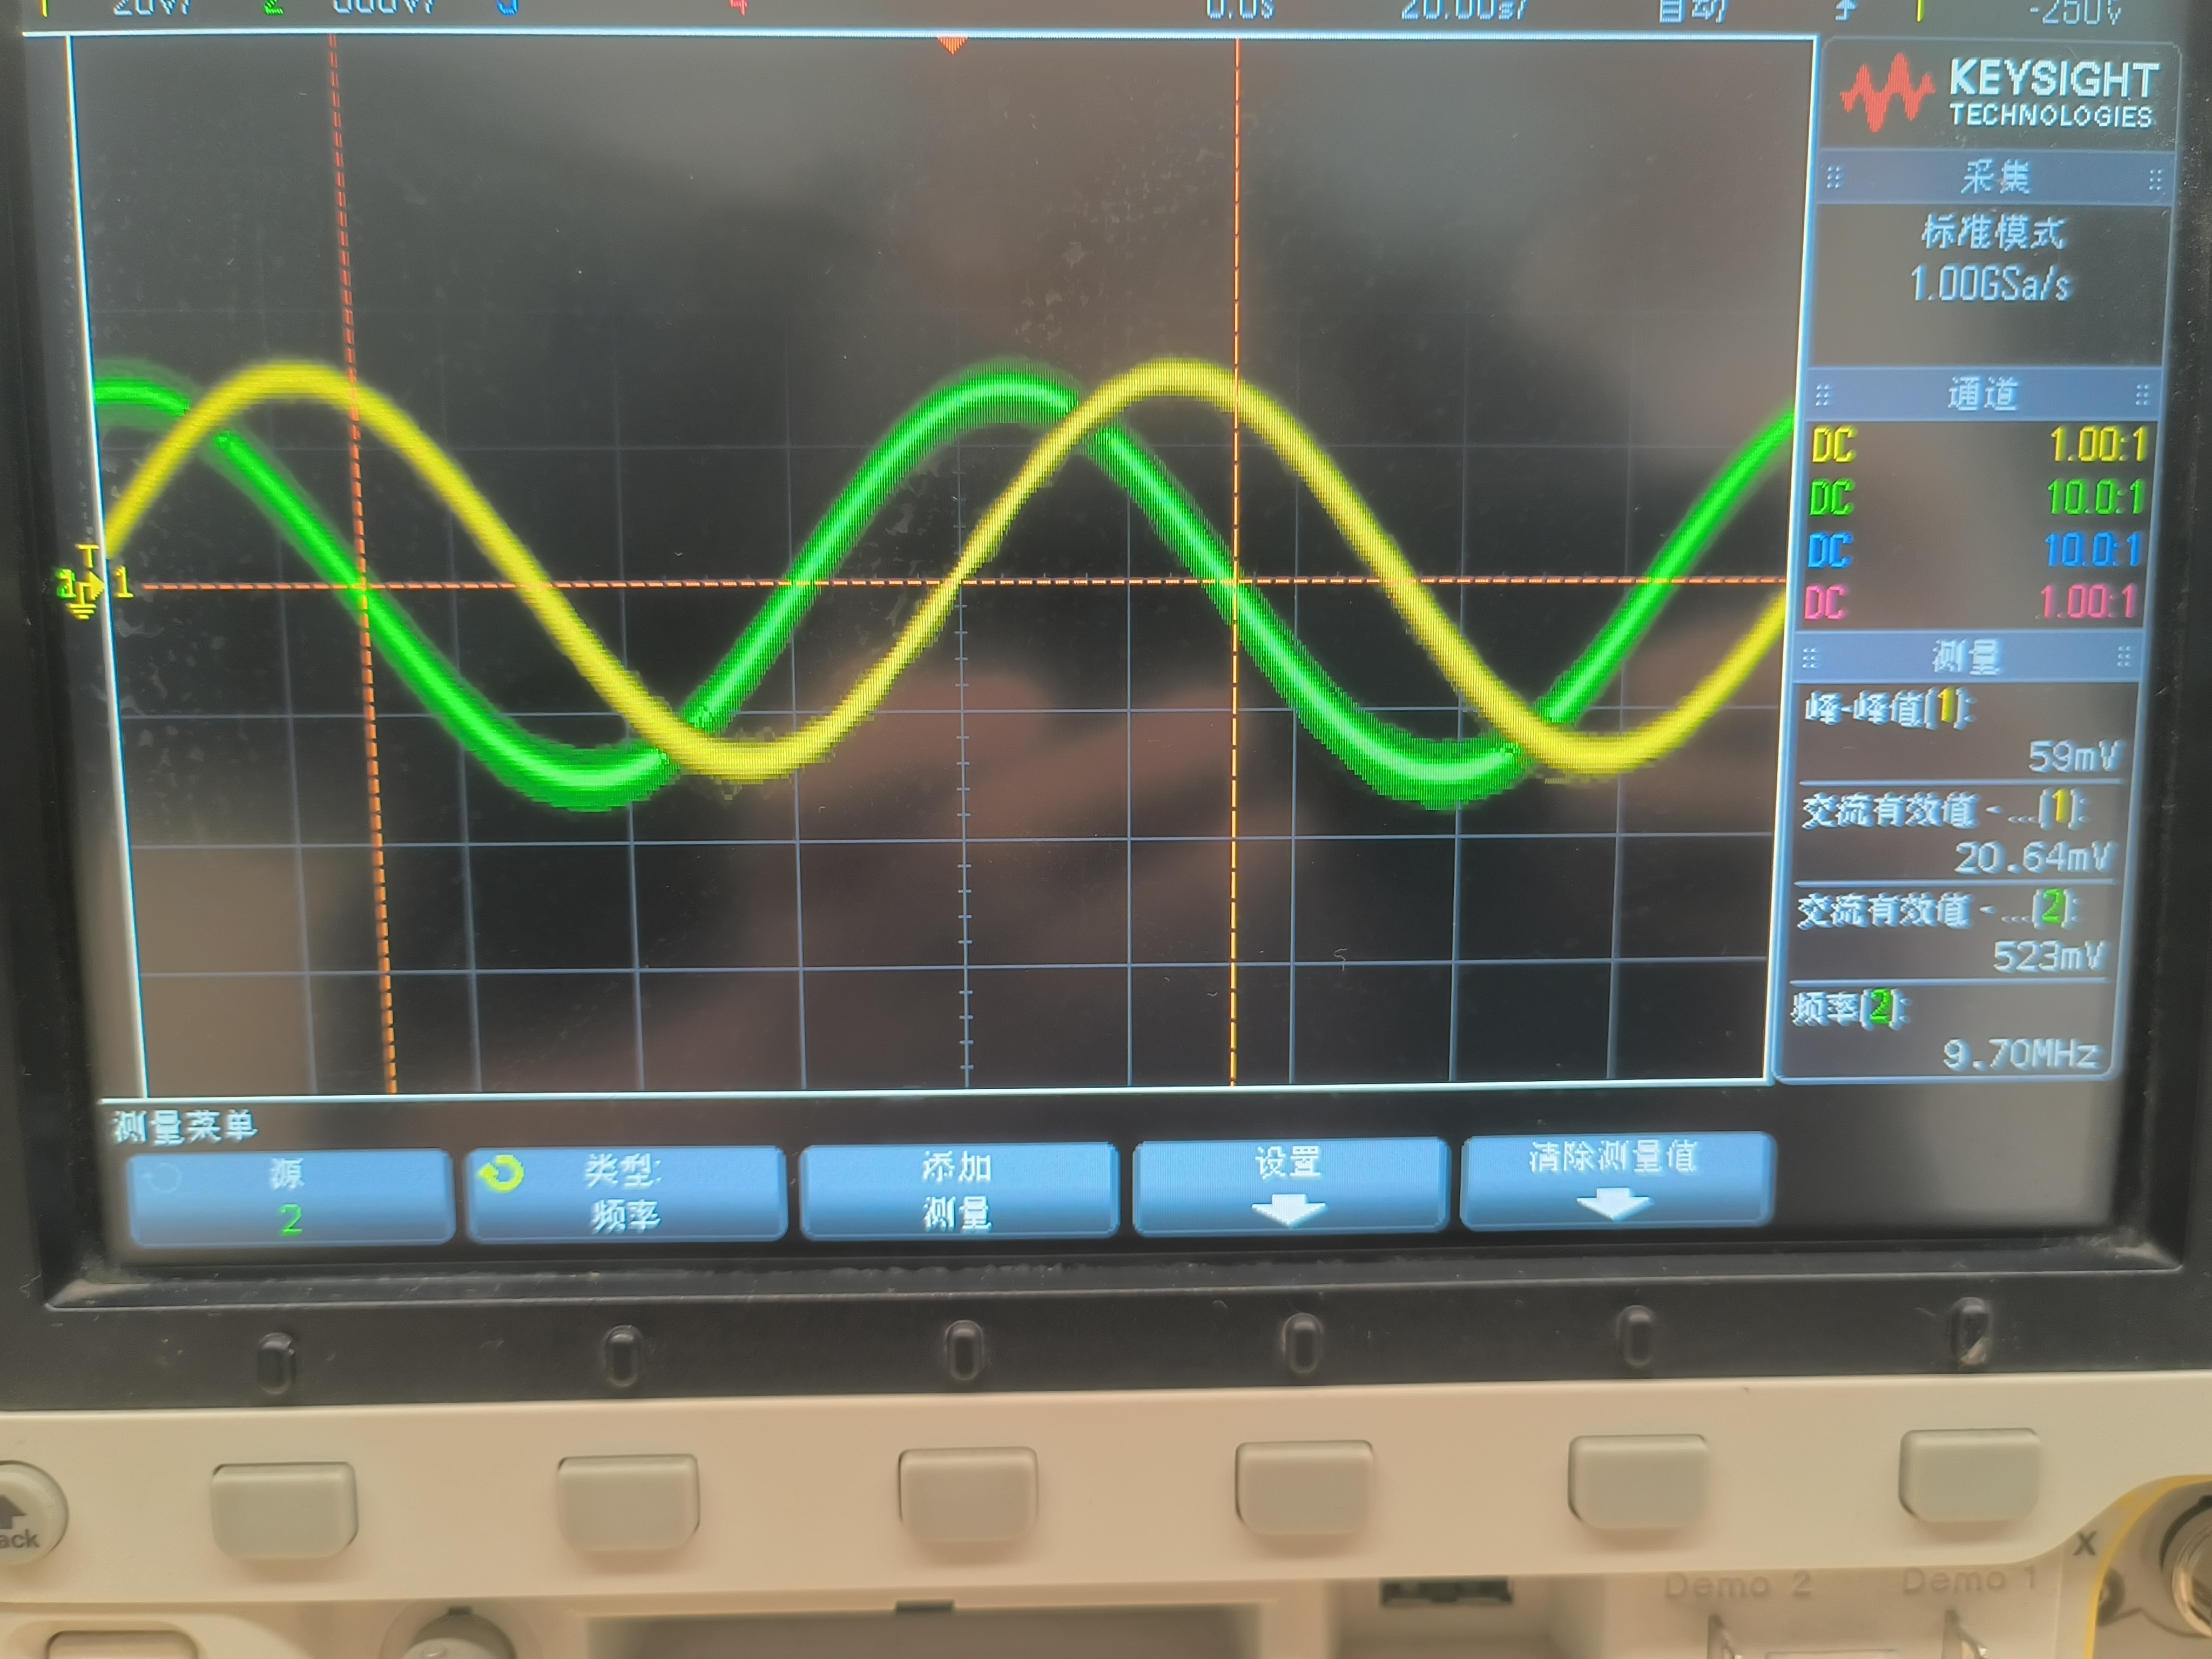
\includegraphics[width=\textwidth]{pics/3.2.2.png}
            \caption{下3dB点时域输入输出波形}\label{3.2.2}
        \end{subfigure}
        \begin{subfigure}[c]{0.45\textwidth}
            \centering
            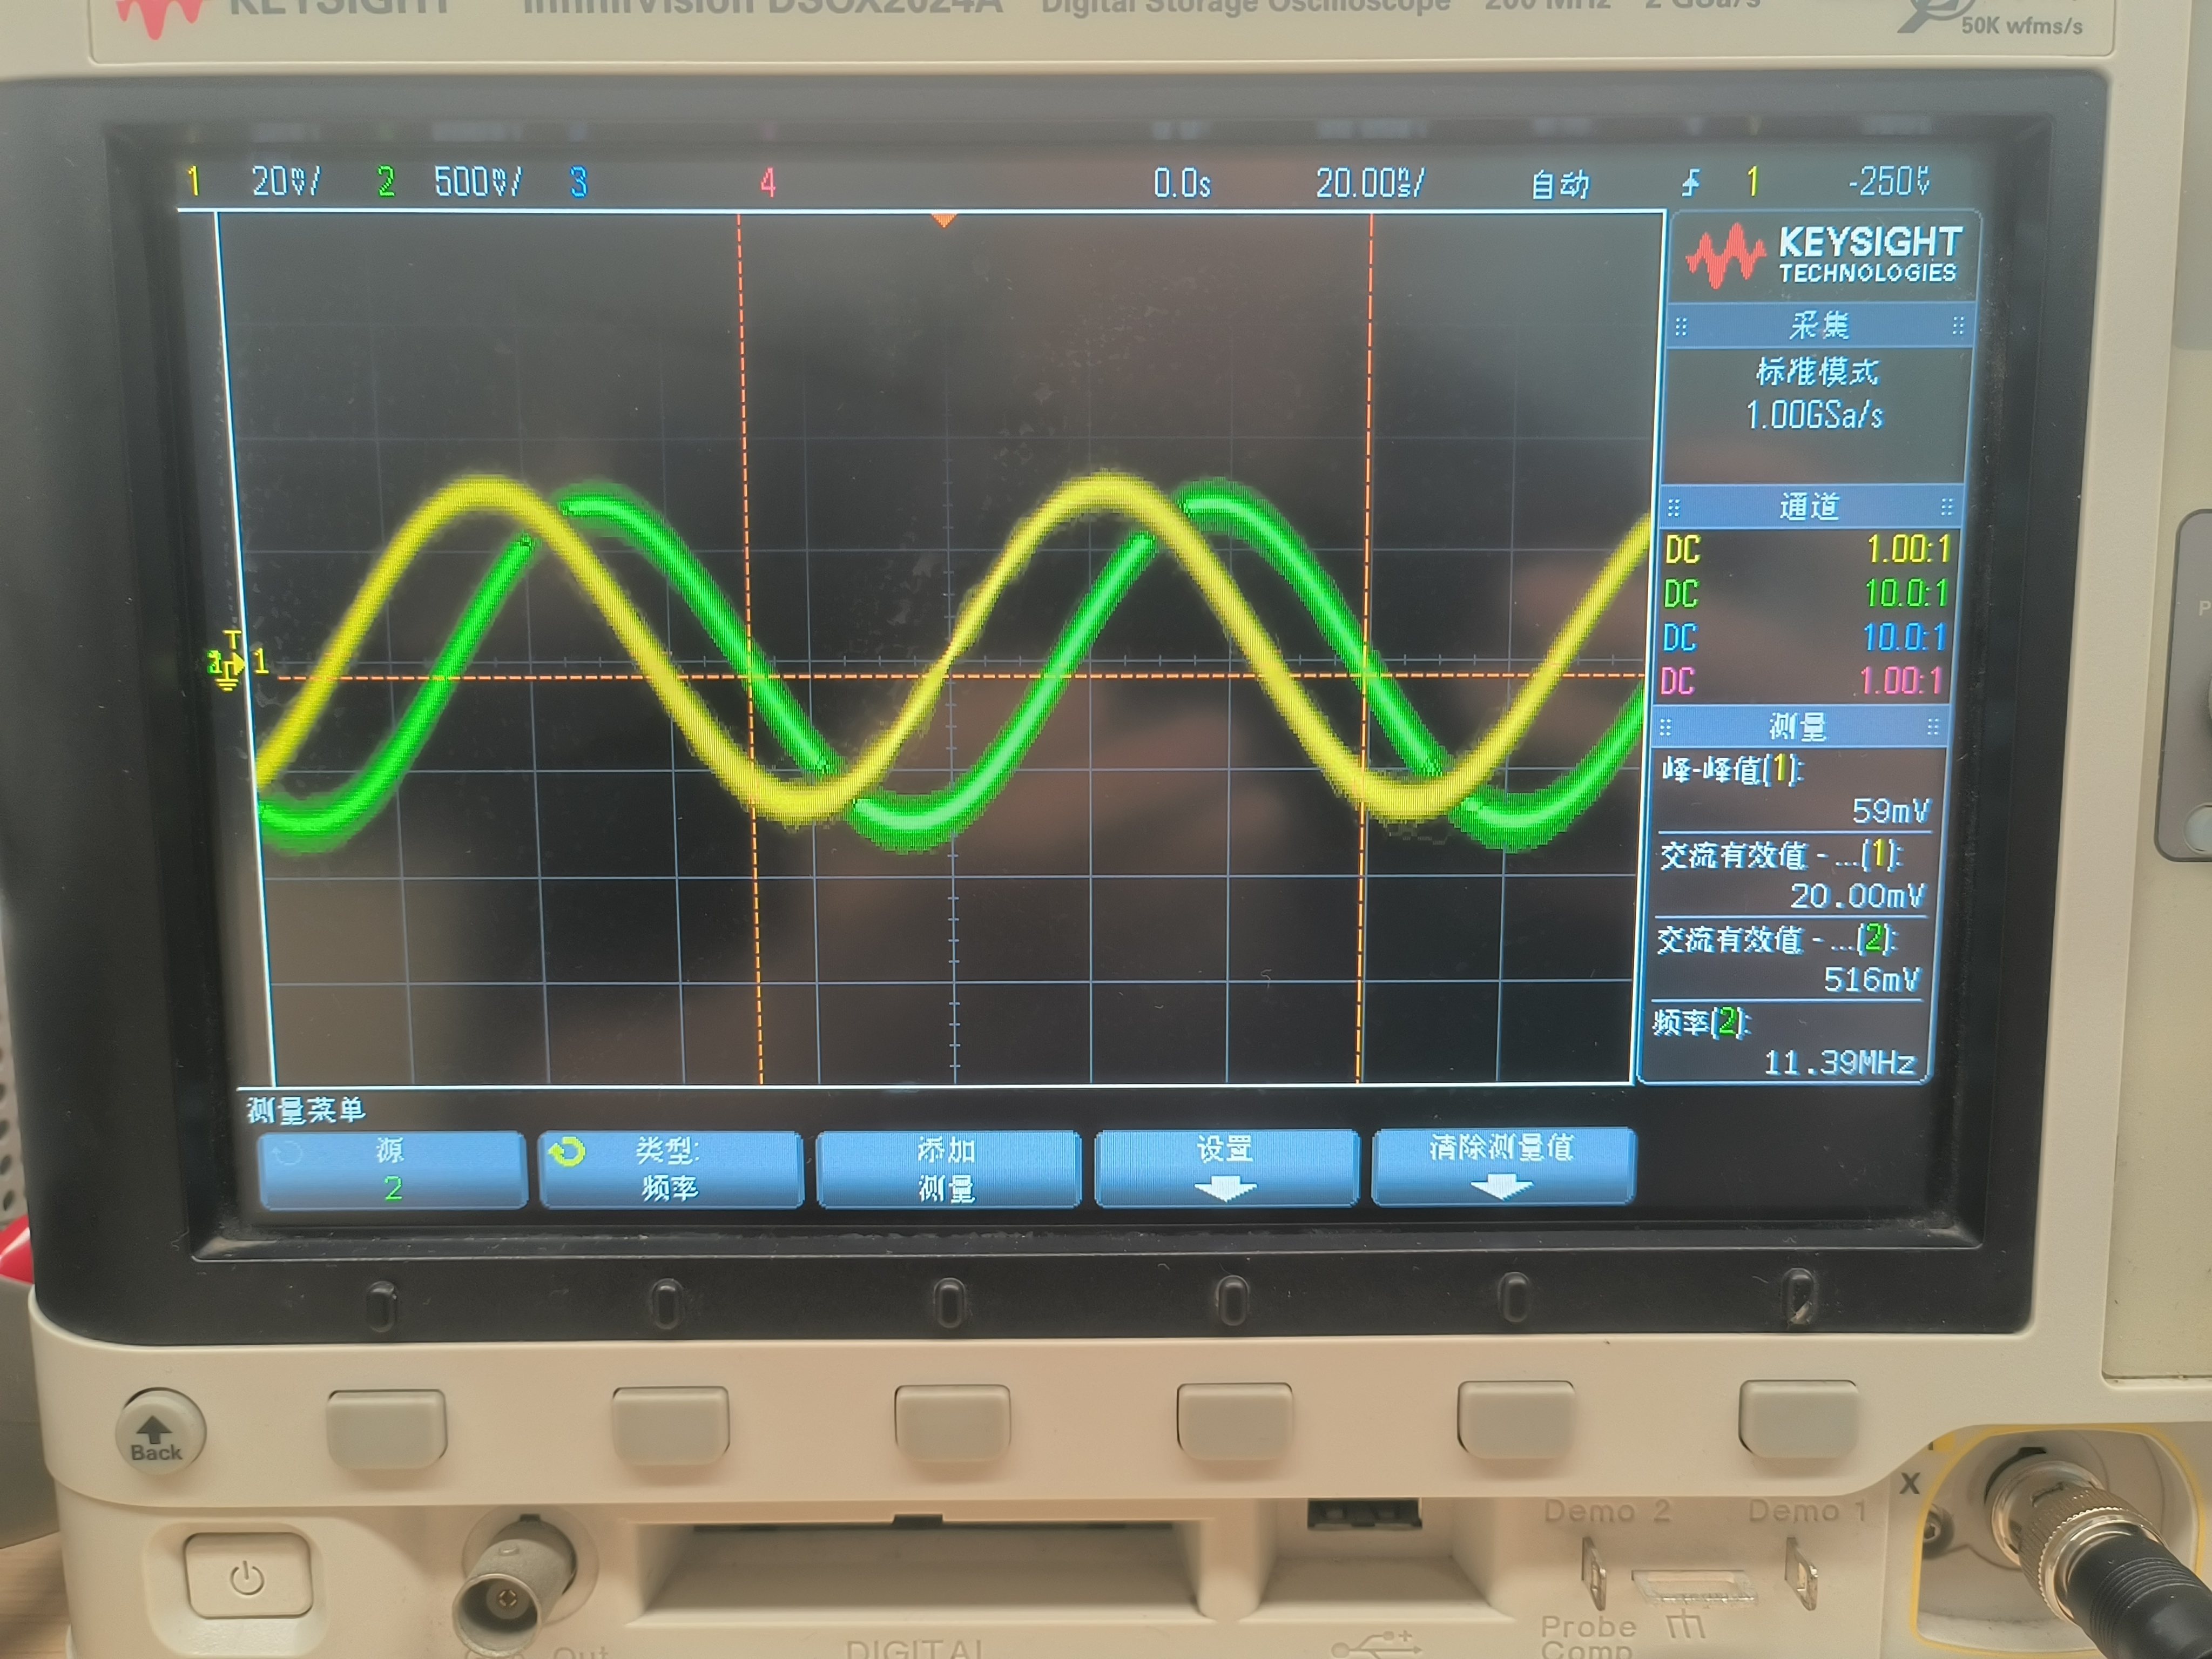
\includegraphics[width=\textwidth]{pics/3.2.2(2).png}
            \caption{上3dB点时域输入输出波形}\label{3.2.2(2)}
        \end{subfigure}
        \caption{单调谐放大器3dB点时域输入输出波形}\label{fig:bi_harmo_amplifier}
    \end{figure}

    \vspace{-2em}
    \textbf{下3dB点:}

    频率$f_L=9.70MHz$,
    输入有效值$U_{iL}=20.64mV$,
    输出有效值$U_{oL}=523mV$,
    谐振电压增益 $A_{VOL}=\dfrac{U_{oL}}{U_{iL}}=25.34=28.08dB$。

    \textbf{上3dB点:}

    频率$f_H=11.39MHz$,
    输入有效值$U_{iH}=20.00mV$,
    输出有效值$U_{oH}=516mV$,
    谐振电压增益 $A_{VOH}=\dfrac{U_{oH}}{U_{iH}}=25.8=28.23dB$。

    $N(3)dB$带宽 $2\Delta f_{0.7}=f_H-f_L=1.69MHz$

\end{enumerate}

\subsection{双调谐放大器频域测量}
\begin{enumerate}[(1)]
    \item \noindent \textbf{强耦合 $N(3)dB$ 带宽}
    
    \begin{figure}[H]
        \centering
        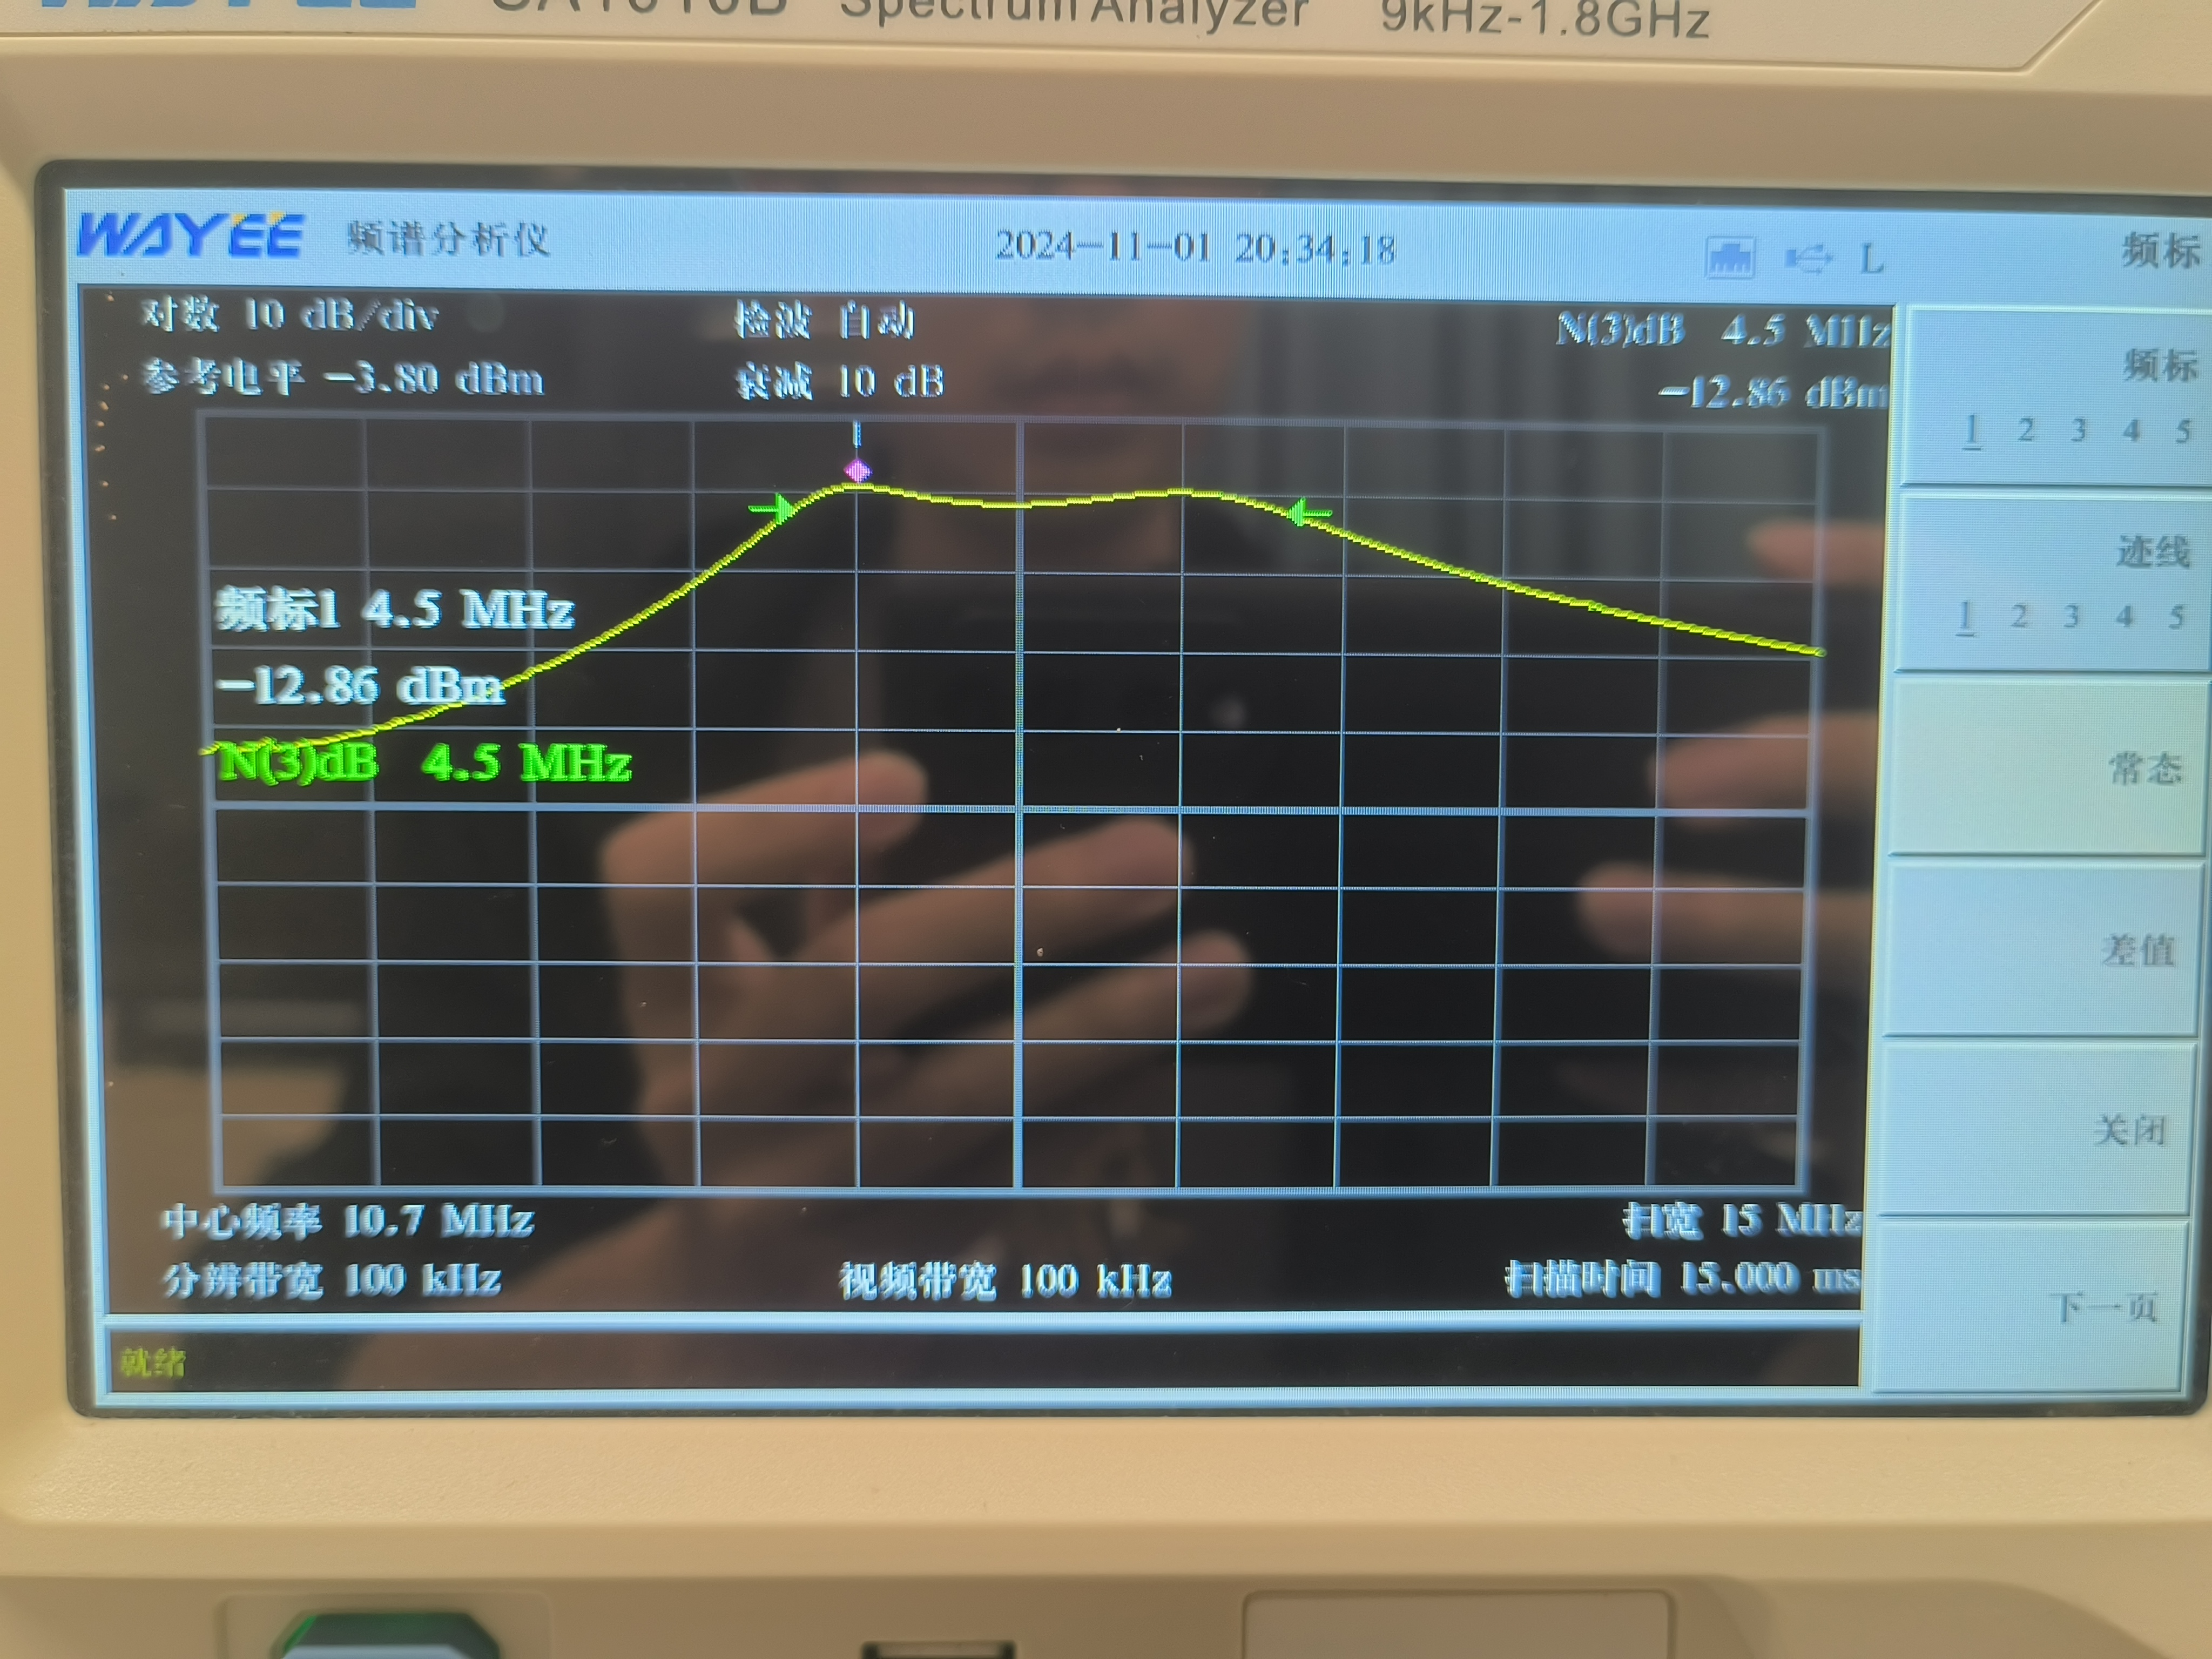
\includegraphics[width=0.45\textwidth]{pics/3.3.1.png}
        ~\\
        \caption{双调谐放大器幅频特性曲线}\label{fig:3.3.1}
    \end{figure}

    \vspace{-2em}
    测量得强耦合$N(3)dB$带宽:
    $2\Delta f_{0.7}=4.5MHz$
    
    \item \noindent \textbf{临界耦合 $N(3)dB$ 带宽 $N(20)dB$ 带宽与矩形系数}

    \begin{figure}[H]
        \centering
        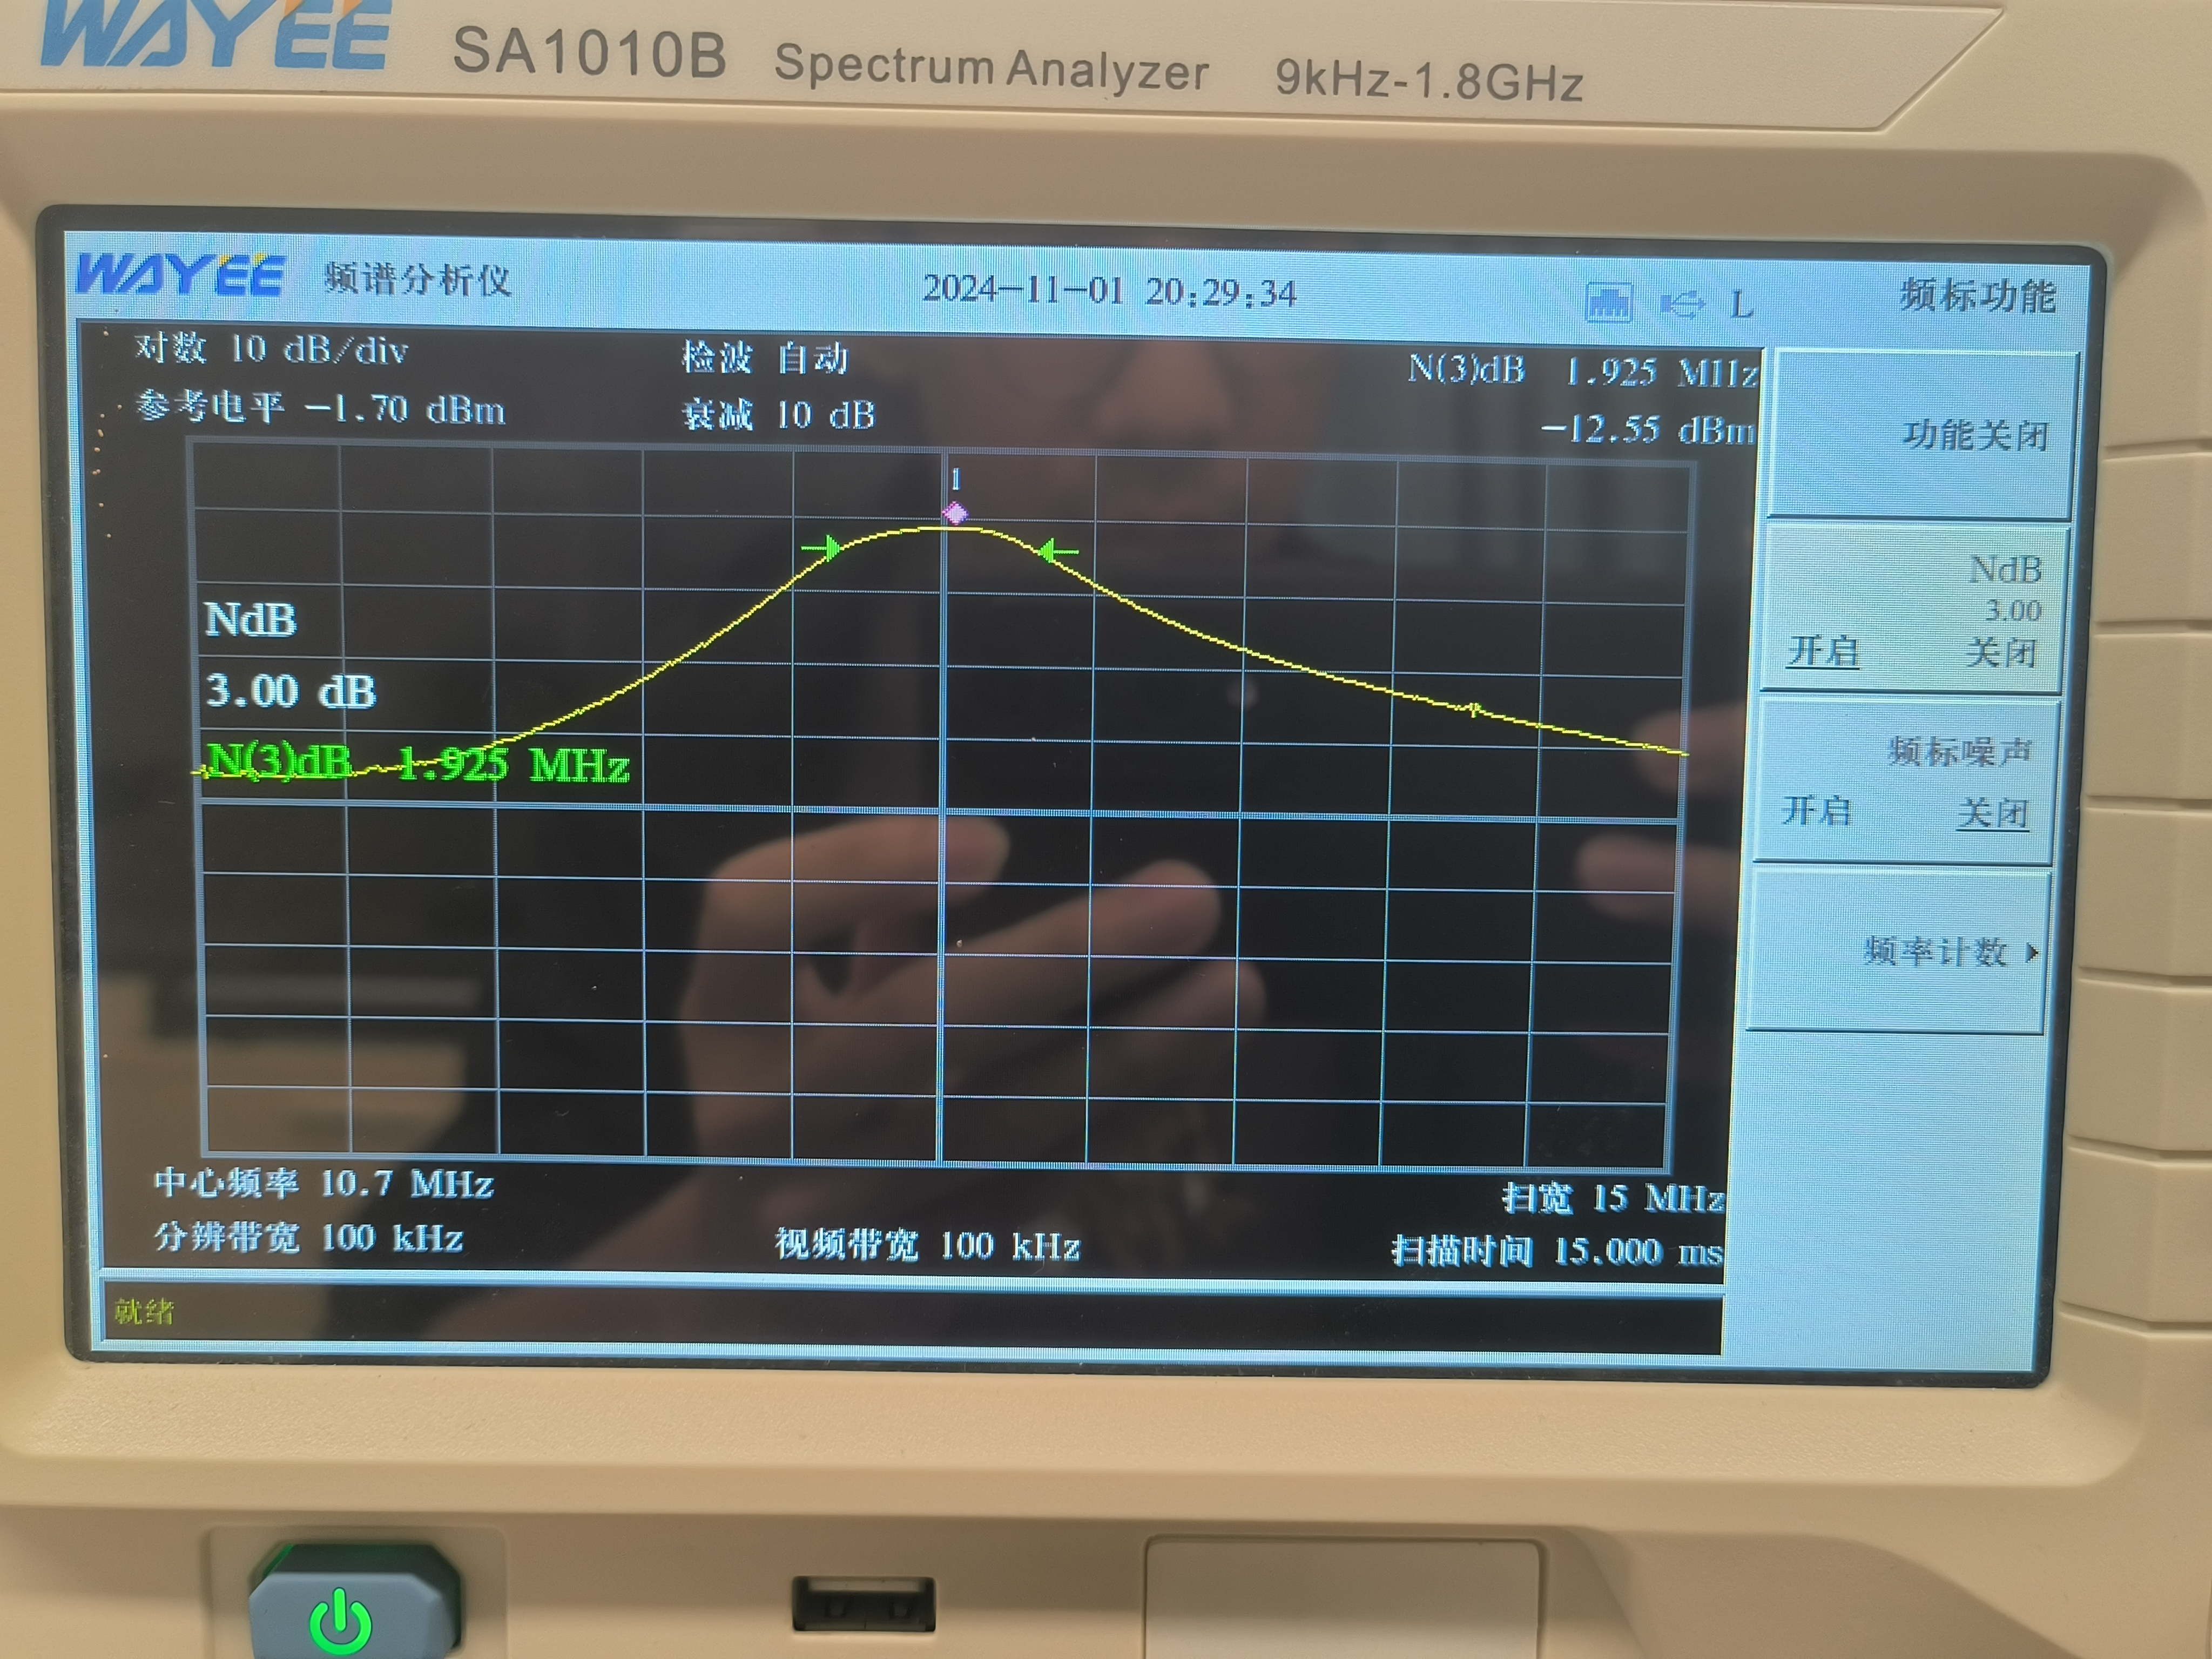
\includegraphics[width=0.45\textwidth]{pics/3.3.2.png}
        ~\\
        \caption{双调谐放大器幅频特性曲线}\label{fig:3.3.2}
    \end{figure}

    \vspace{-2em}
    测量得临界耦合$N(3)dB$带宽为
    $2\Delta f_{0.7}=1.925MHz$,$N(20)dB$带宽为
    $2\Delta f_{0.1}=6.8MHz$,
    矩形系数为
    $K_{r0.1}=\dfrac{2\Delta f_{0.1}}{2\Delta f_{0.7}}=3.532$
    
    \item \noindent \textbf{临界耦合 谐振电压增益 $A_{VO}$}

    此处由于疏忽未拍照,但记录了谐振电压增益 $A_{VO}=18.72dB$。

    如果考虑频谱仪上标注的衰减10dB,此时实际电压增益应为$A_{VO}=28.72dB$  
    
\end{enumerate}
\subsection{双调谐放大器时域测量}
\begin{enumerate}[(1)]
    \item \noindent\textbf{谐振电压增益 $A_{VO}$}
    
    \begin{figure}[H]
        \centering
        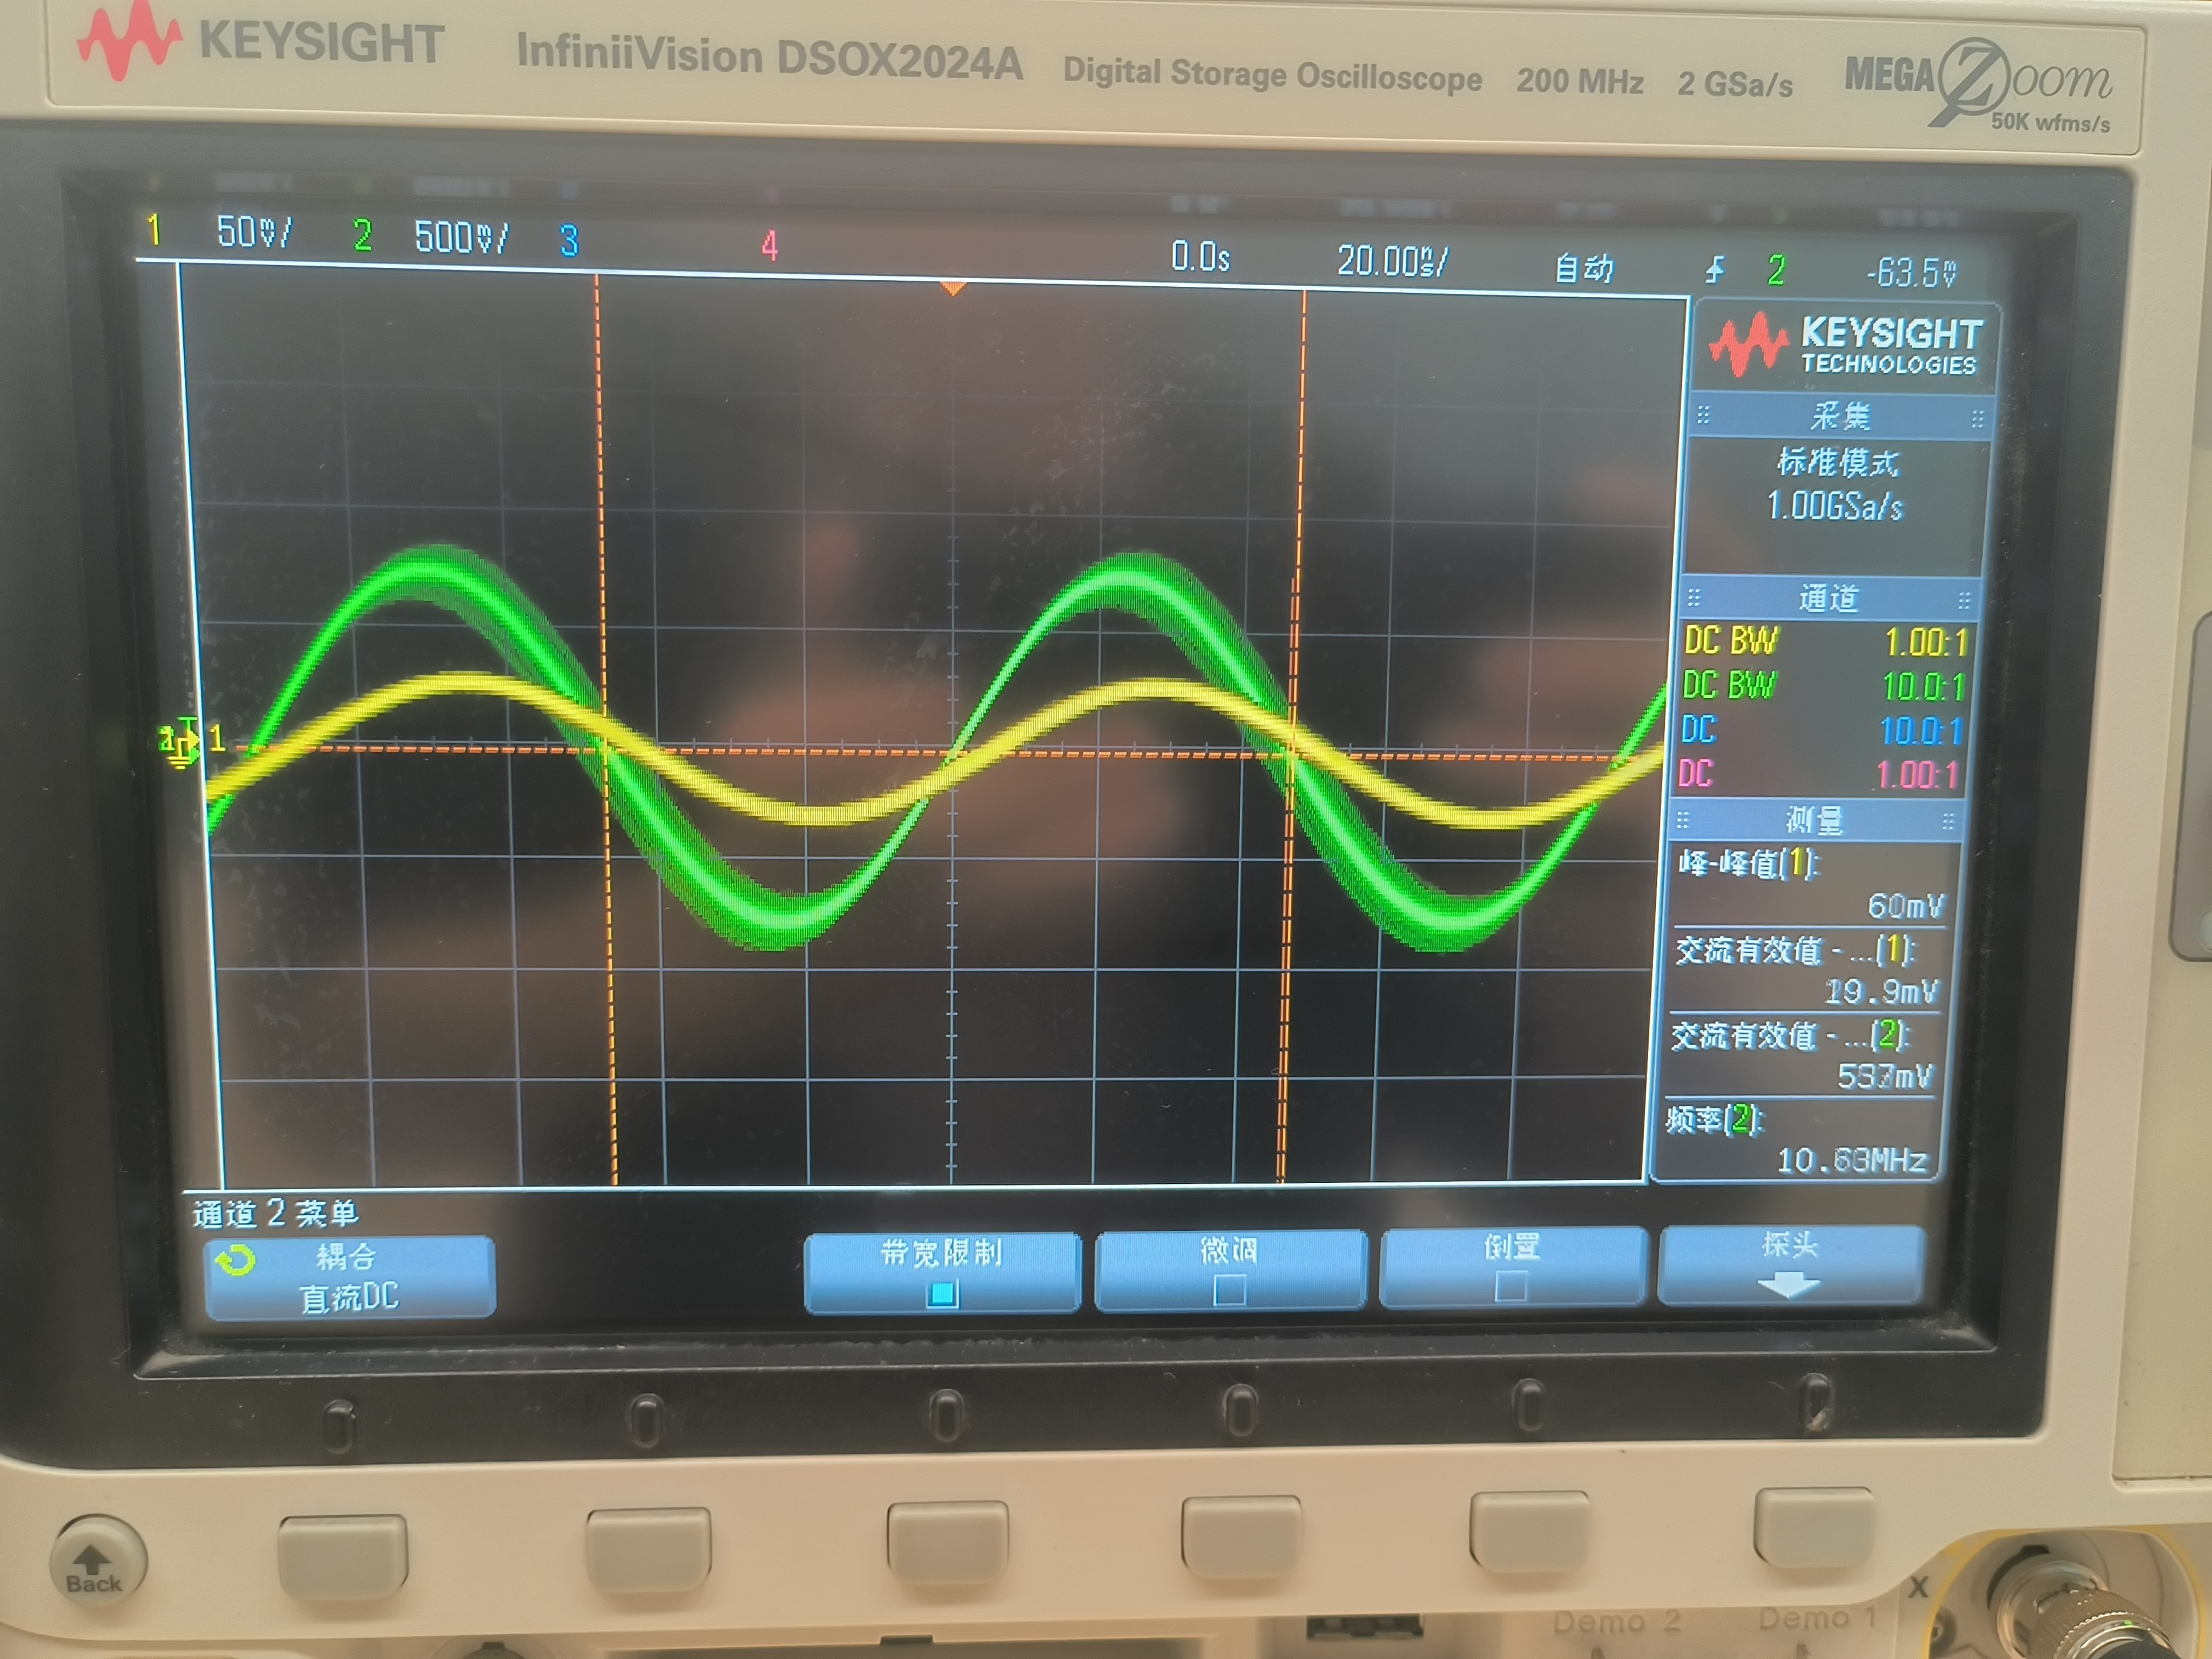
\includegraphics[width=0.45\textwidth]{pics/3.4.1.png}
        ~\\
        \caption{双调谐放大器时域输入输出波形}\label{fig:3.4.1}
    \end{figure}

    
    输入有效值$U_i=19.9mV$,输出有效值$U_o=537mV$,谐振电压增益 $A_{VO}=\dfrac{U_o}{U_i}=26.98=28.62dB$。
    
    与频域测得的电压增益28.72dB(考虑频谱仪衰减)相比较,误差在合理范围内。
    \item \noindent\textbf{$N(3)dB$ 通频带}

    \begin{figure}[H]
        \centering
        \begin{subfigure}[c]{0.45\textwidth}
            \centering
            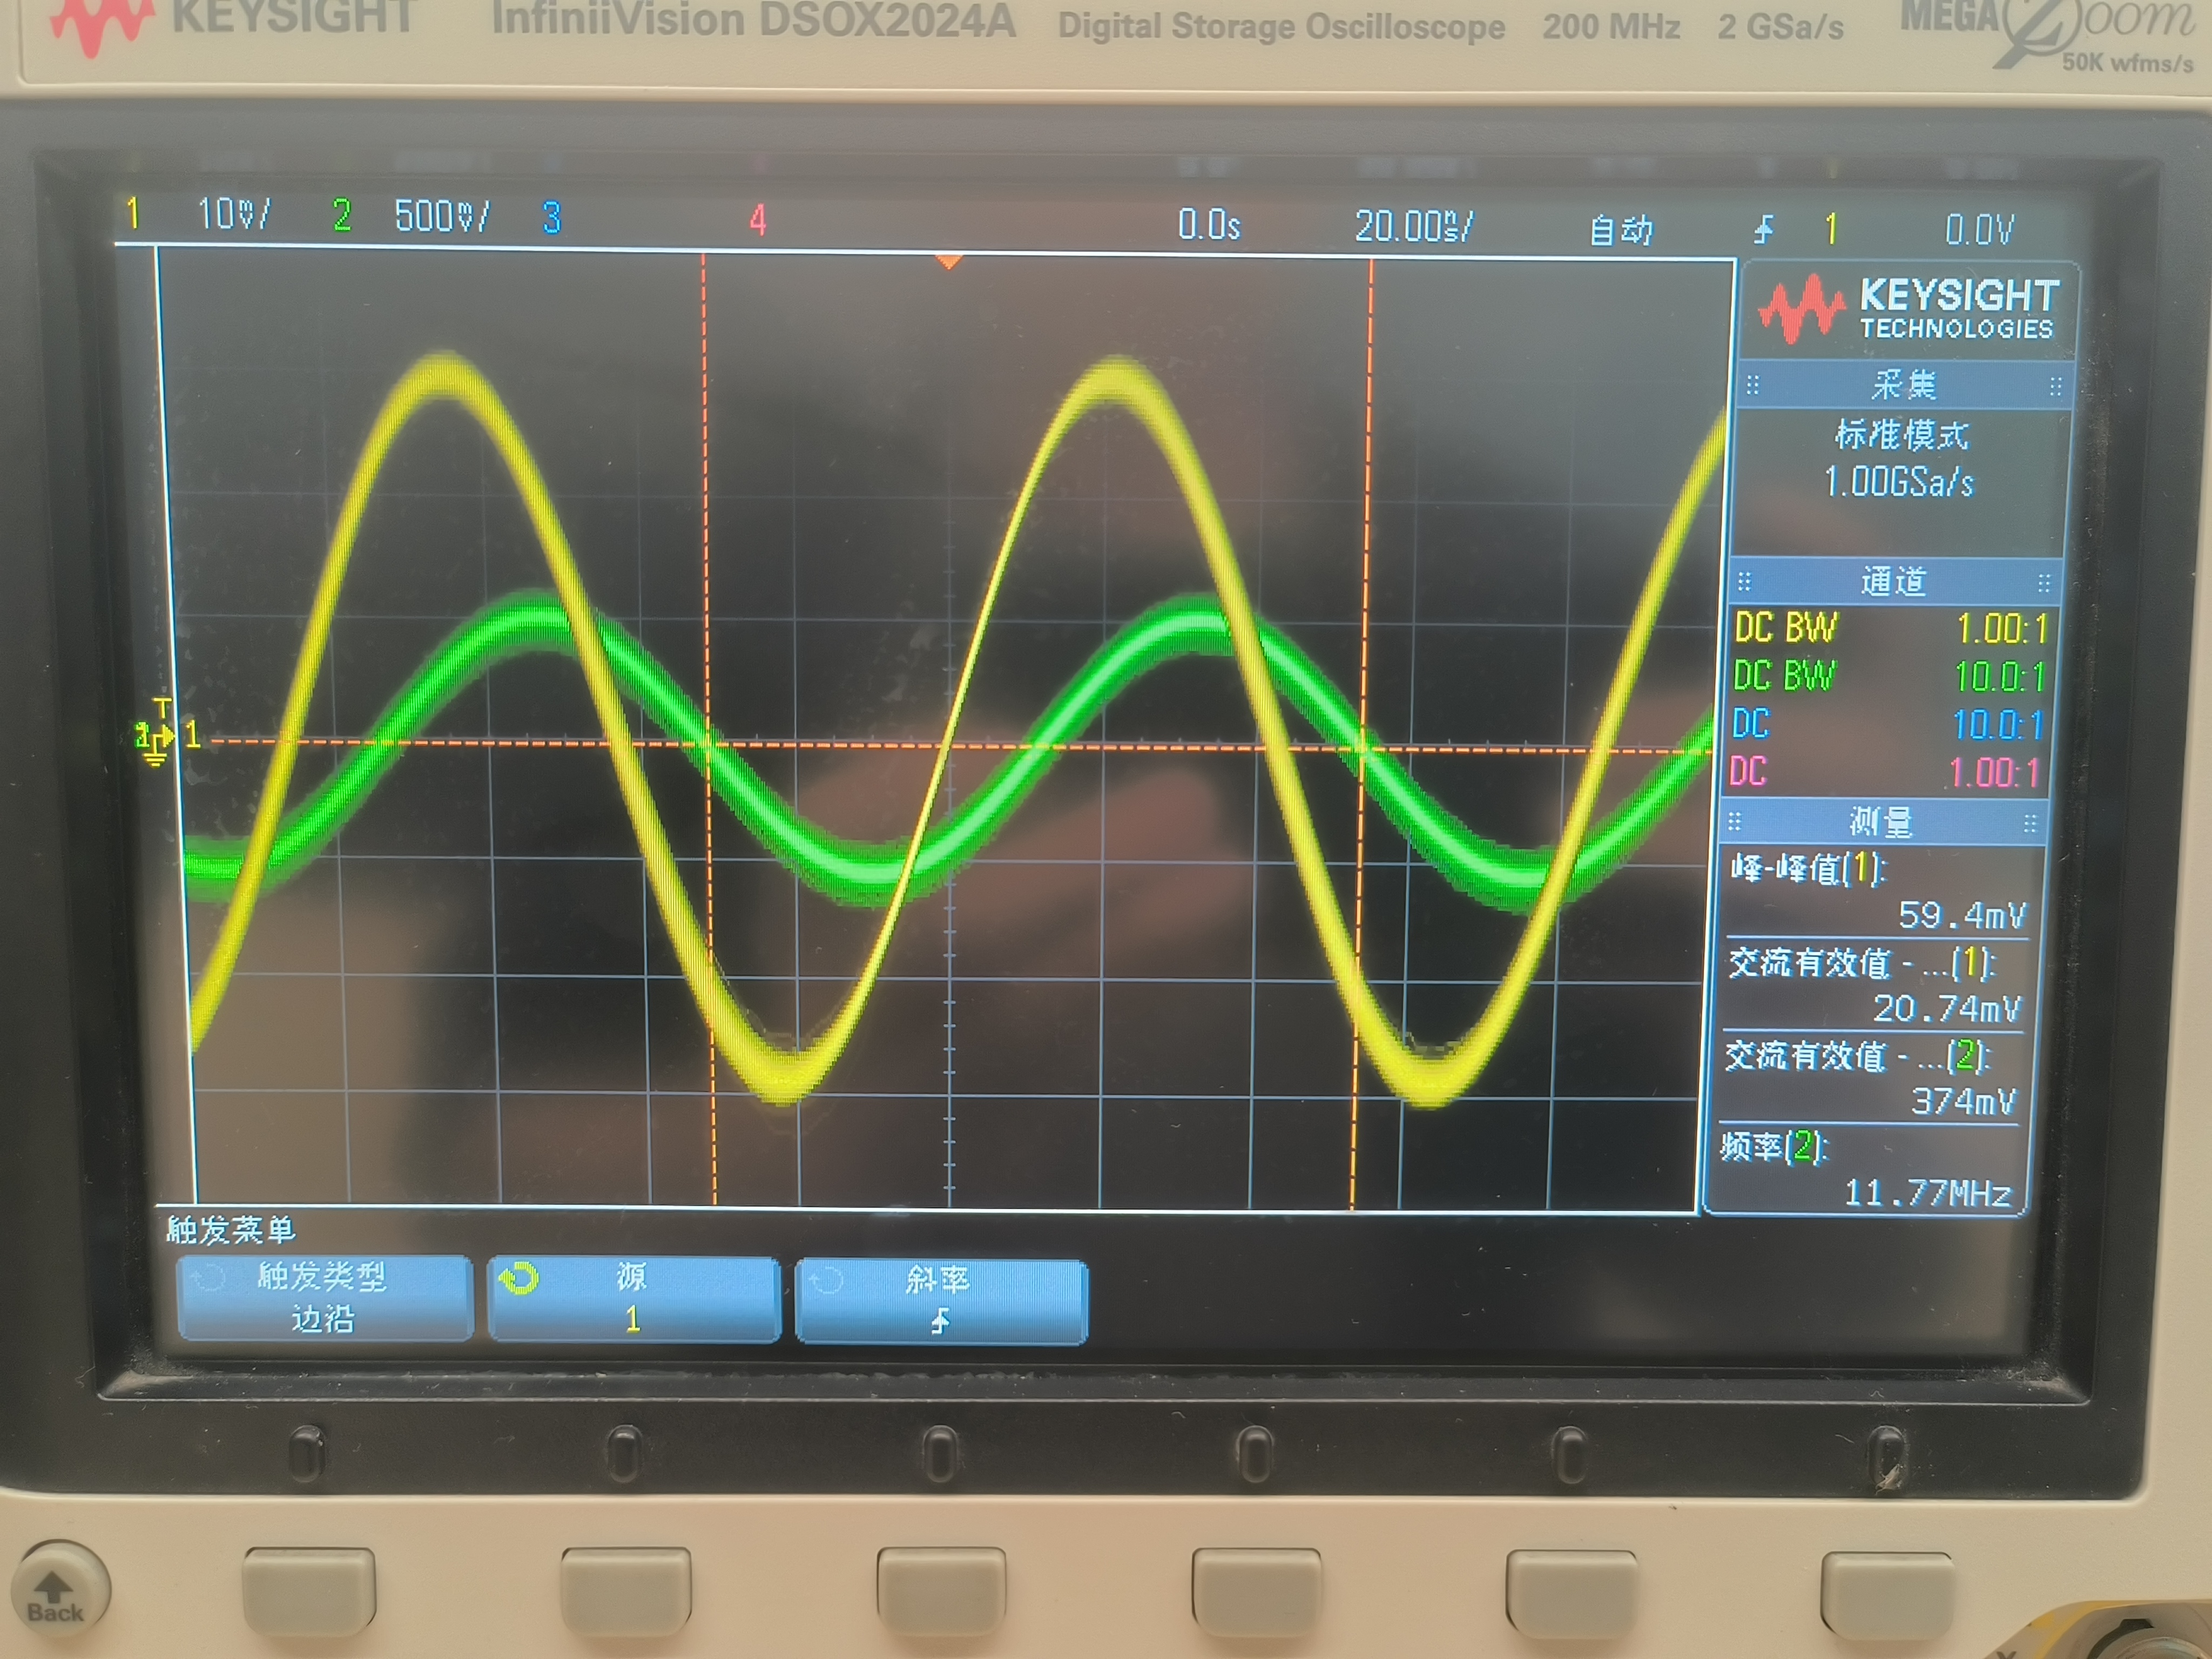
\includegraphics[width=\textwidth]{pics/3.4.2.png}
            \caption{下3dB点时域输入输出波形}\label{3.4.2}
        \end{subfigure}
        \begin{subfigure}[c]{0.45\textwidth}
            \centering
            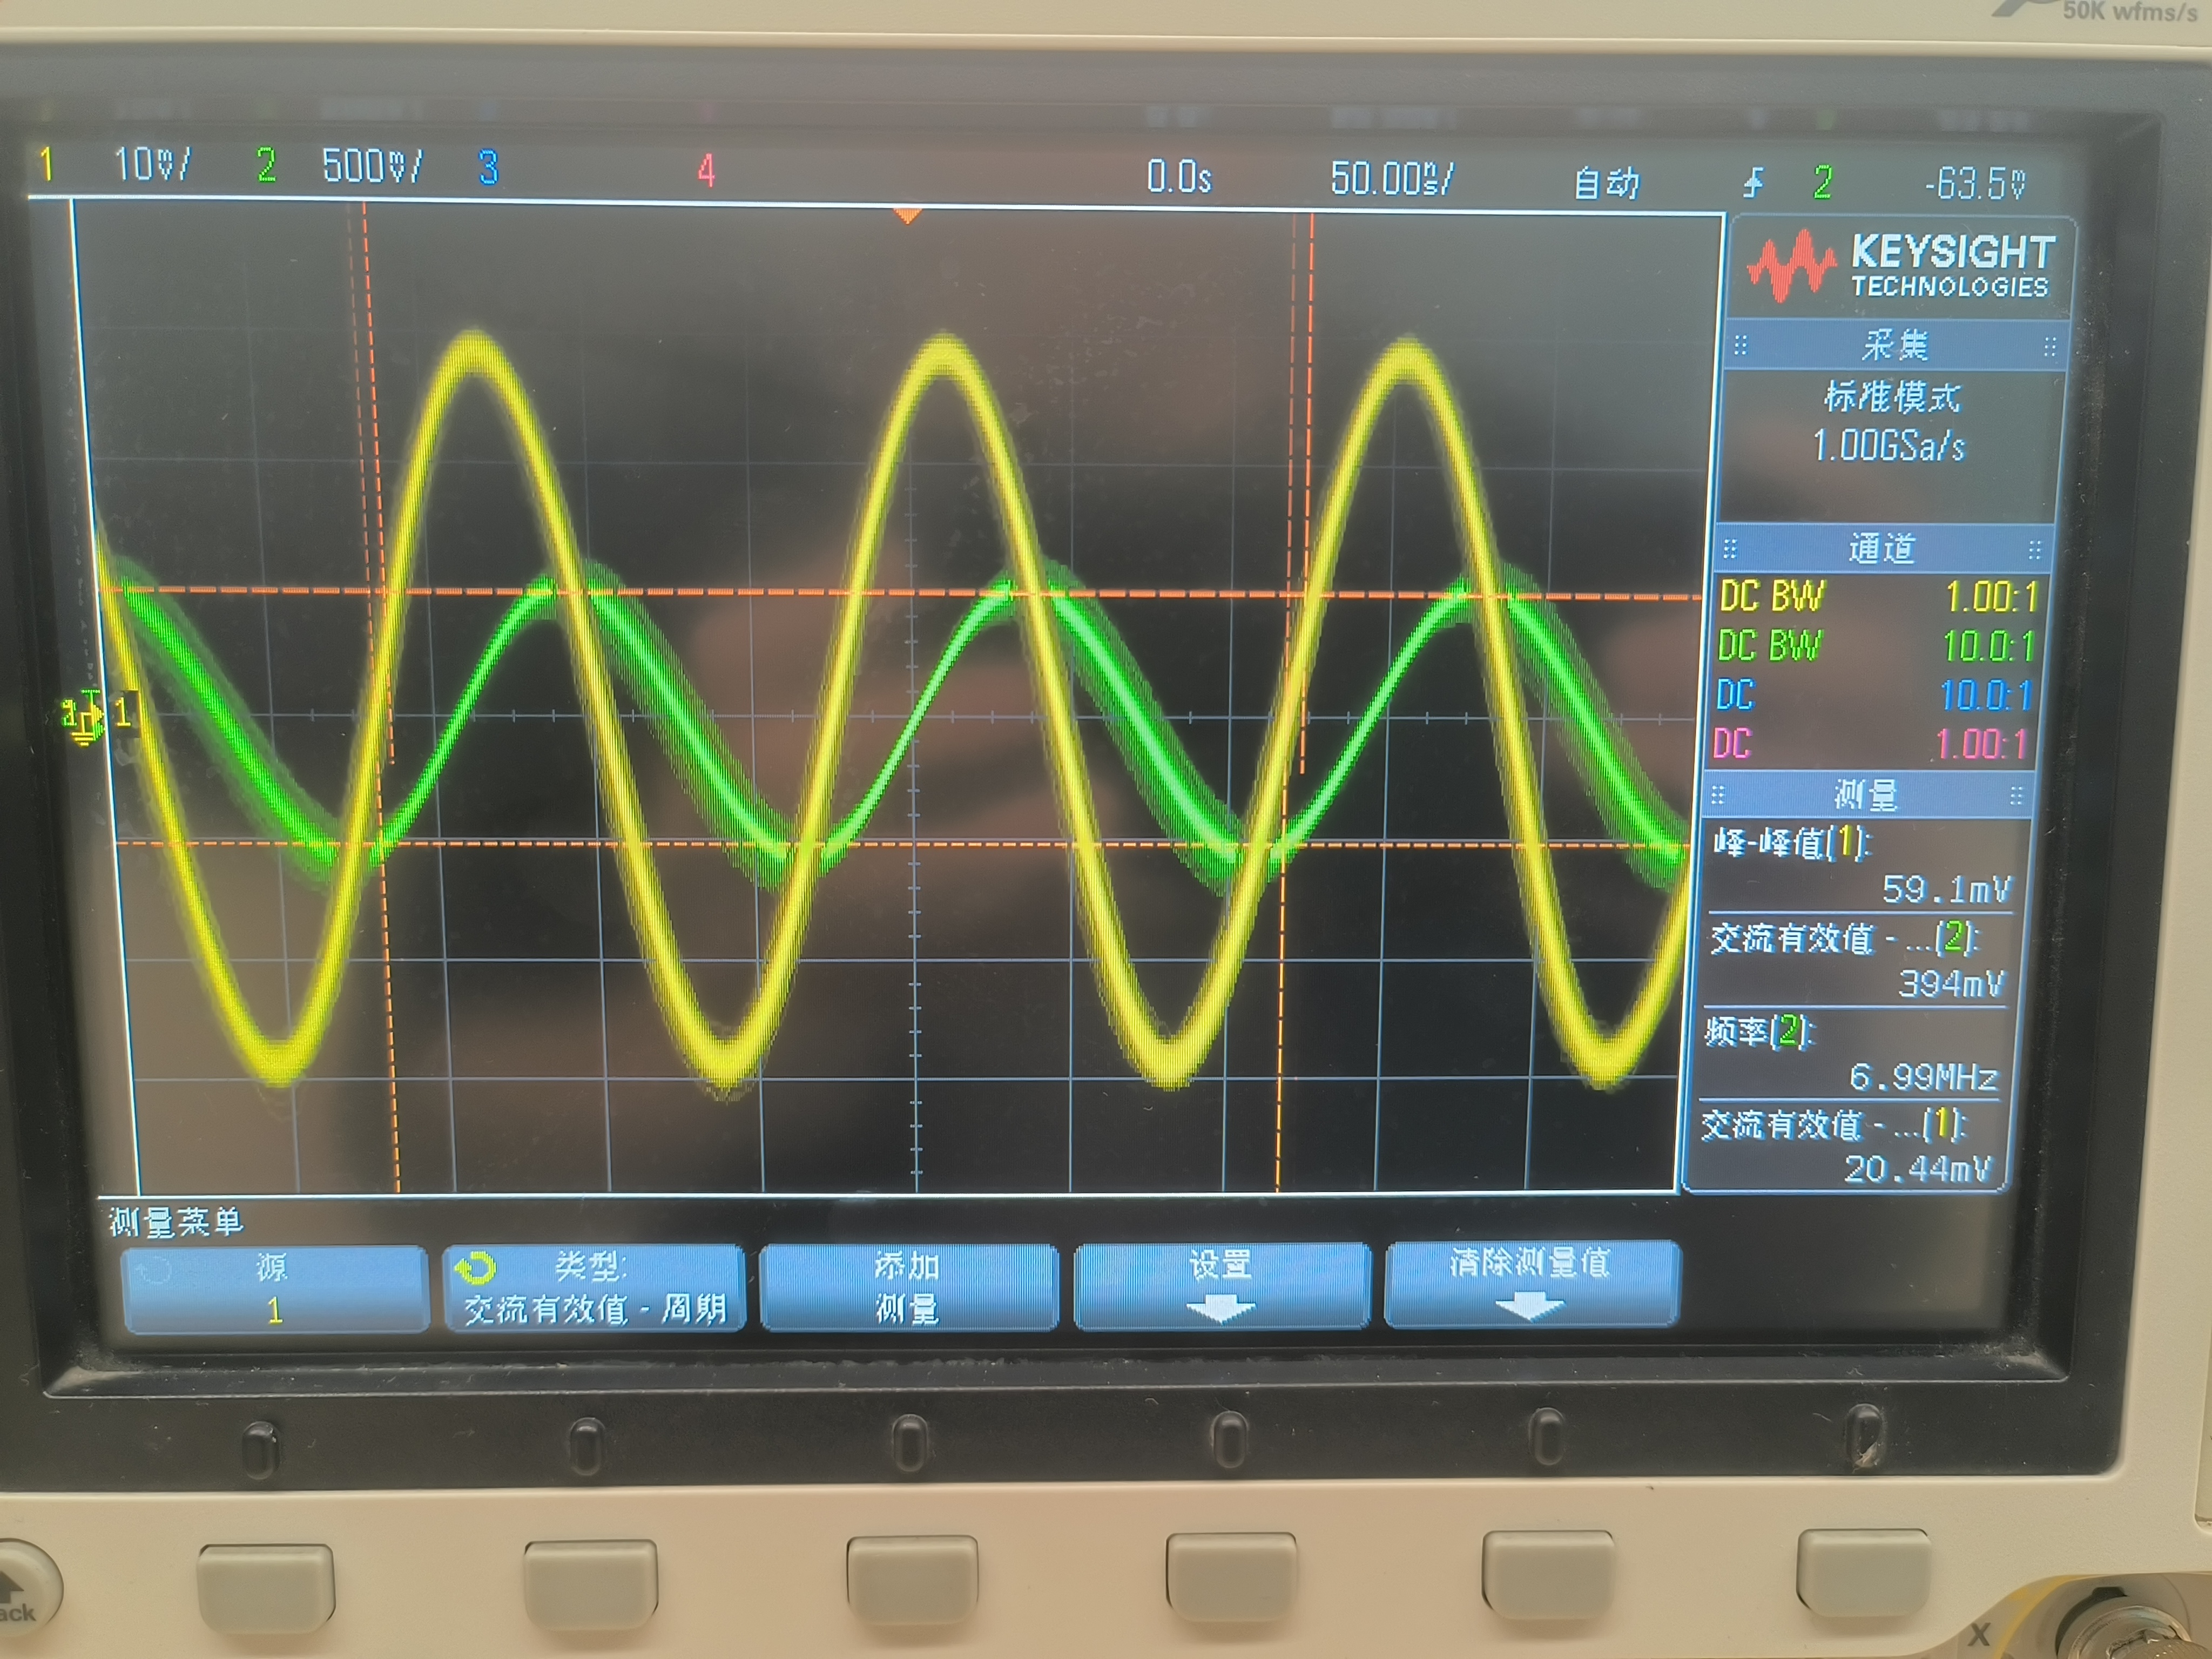
\includegraphics[width=\textwidth]{pics/3.4.2(2).png}
            \caption{上3dB点时域输入输出波形}\label{3.4.2(2)}
        \end{subfigure}
        
        \caption{双调谐放大器3dB点时域输入输出波形}\label{3.4.2-}
    \end{figure}

    \vspace{-2em}
    \textbf{下3dB点:}

    频率$f_L=6.99MHz$,
    输入有效值$U_{iL}=20.44mV$,
    输出有效值$U_{oL}=394mV$,
    谐振电压增益 $A_{VOL}=\dfrac{U_{oL}}{U_{iL}}=19.28=25.70dB$。

    \textbf{上3dB点:}

    频率$f_H=11.77MHz$,
    输入有效值$U_{iH}=20.74mV$,
    输出有效值$U_{oH}=374mV$,
    谐振电压增益 $A_{VOH}=\dfrac{U_{oH}}{U_{iH}}=18.03=25.12dB$。

    $N(3)dB$带宽 $2\Delta f_{0.7}=f_H-f_L=1.69MHz$
    
\end{enumerate}

\section{第四部分 \texorpdfstring{\quad}{} 思考题}
\begin{enumerate}[I.]
    \item \textbf{比较时域测量与频域测量的特点。}
    
    答:
    \textbf{(1)时域测量主要关注信号随时间的变化,通常使用示波器进行测量。}

    时域测量可以直观地显示电压或电流随时间的变化,在分析信号的周期、上升下降边沿、周期、延迟、波形失真等指标时有优势。
    缺点是对于复杂信号难以直接从时域波形中观察出频率成分或周期性特征。
   
    \textbf{(2)频域测量主要分析信号在不同频率下的分布情况,通常使用频谱仪进行测量。}
    
    频域测量能够展示信号的频率成分和对应幅值,在针对周期信号、复杂信号的分析中更有优势。通过观察信号频谱能够进行信号带宽等指标的测量。
    
    \item \textbf{分析阻尼电阻 $R_{12}$ 对单调谐放大器性能的影响(如通频带、矩形系数和谐振电压增益)。}

    答:
    理论上分析可以得到,阻尼电阻$R_12$接入后会使得$Q_3$集电极的并联谐振回路$Q$值减小,通频带展宽。阻尼电阻增加了能量损耗,因此接入阻尼电阻会导致增益下降。
    
    由实验结果可以看出,接入阻尼电阻后,单调谐放大器的中心频率幅值由69.48mV变为44.97mV,谐振电压增益由20.01dB变为27.63dB,$N(3)dB$带宽由1.15MHz变为1.725MHz,$N(20)dB$带宽由9.675MHz变为12.725MHz,矩形系数由8.413变为7.377,整体趋势为增益下降,通带展宽,矩形系数减小,频率选择性上升。

    \item \textbf{比较单调谐放大器和双调谐放大器(临界耦合)选择性的优劣。}
    
    答:
    不接入阻尼电阻时的单调谐放大器矩形系数为8.413,接入阻尼电阻的单调谐放大器矩形系数为7.377,均大于临界耦合时的双调谐放大器矩形系数3.532,矩形系数越小,选择性越好,因此临界耦合双调谐放大器的选择性更好。

    \item \textbf{分析强耦合时谐振曲线凹陷深度的影响因素。}

    答:强耦合时谐振曲线凹陷深度的影响因素如下:

    (1)$C_{18}$电容值,容值越大耦合越强,谐振曲线凹陷程度越深。
    
    (2)$W_1$和$W_2$值,改变初级和次级回路变容管上的直流电压以改变其电容,从而改变耦合程度和谐振曲线凹陷程度。
\end{enumerate}

\end{document}